\chapter{Análisis y resultados}
En este capítulo se van a discutir los resultados obtenidos tras realizar los experimentos descritos en el capítulo anterior. Se mostrarán gráficas que ilustren la curva de convergencia de los algoritmos en algunos conjunto de datos, para cada clasificador (kNN y SVC) y en cada versión del algoritmo, es decir, original y versión binaria. Junto a eso también se han elaborado una gráficas de ``cajas y bigotes'' o \textit{boxplots} que ilustran no solo los mejores resultados, sino su robustez y estabilidad tras varias iteraciones. \\[6pt]
Además se mostrarán tablas y gráficas de los ranking obtenidos en versión binaria y en versión continua para cada clasificador tras hacer la media de los resultados en todos los conjuntos de datos.\\[6pt]
Por último, los resultados vendrán expuestos en forma de tabla junto a las métricas correspondientes, de forma que se facilite el análisis de los algoritmos, de las versiones reales y continuas y de los clasificadores usados.\\[6pt]
También ser realizarán análisis estadísticos de los resultados obtenidos utilizando como herramienta la página web \textbf{TACOlab}~\cite{taco_website}, facilitada por el tutor del proyecto, de forma que se puedan hacer los mejores y más robustos tests de forma automática y sencilla.\\[6pt]
Como detalle a tener en cuenta, se ha añadido en las comparaciones un optimizador al que se le ha llamado ``Dummy'', debido a su naturaleza totalmente aleatorio y sin criterio alguno. Se añade como algoritmo de referencia, ninguna otra metaheurística debería ser peor que esta en promedio. En caso contrario podría decirse que el algoritmo en cuestión está mal diseñado.\\[6pt]
Pese a que se dividirán los análisis entre binario y continuo, las versiones discretas se escribirán con la letra \textit{b} delante. Por ejemplo, el algoritmo \textbf{FA} en binario sería \textbf{bFA}.

\section{Binario}
En esta sección se discutirán y analizarán los resultados para las metaheurísticas de codificación binaria o discreta. Estas versiones tienen un enfoque del problema distinto al de las reales, pues codifican cada característica con un $0$ o un $1$, o lo que es lo mismo, descartan características. Dada su naturaleza, cabría pensar que son los algoritmos más específicos que podrían usarse para el problema se selección de características.

\subsection{General}
En esta sub-sección se presentarán los resultados generales obtenidos con las metaheurísticas binarias. Esto permitirá una visión más amplia de su desempeño y proporcionará intuiciones iniciales sobre la efectividad de cada algoritmo en distintos contextos.

\begin{figure}[htb]
    \centering
    \includegraphics[width=\textwidth]{imagenes/fitness_charts/results/binary/ionosphere/optimizer_boxplot_fitness_knn_b.png}
    \caption{Boxplot ionosphere en kNN - binario}
    \label{fig:boxplot_ionosphere}
\end{figure}

\begin{figure}[htb]
    \centering
    \includegraphics[width=\textwidth]{imagenes/fitness_charts/results/binary/wdbc/optimizer_boxplot_fitness_knn_b.png}
    \caption{Boxplot wdbc en kNN - binario}
    \label{fig:boxplot_wdbc}
\end{figure}

\begin{figure}[htb]
    \centering
    \includegraphics[width=\textwidth]{imagenes/fitness_charts/results/binary/diabetes/optimizer_boxplot_fitness_knn_b.png}
    \caption{Boxplot diabetes en kNN - binario}
    \label{fig:boxplot_diabetes}
\end{figure}

\begin{figure}[htb]
    \centering
    \includegraphics[width=\textwidth]{imagenes/fitness_charts/results/binary/parkinsons/optimizer_boxplot_fitness_knn_b.png}
    \caption{Boxplot parkinsons en kNN - binario}
    \label{fig:boxplot_parkinsons}
\end{figure}

Como ya se aclaró en capítulos anteriores, para obtener estos resultados se han ejecutado $10$ veces cada algoritmo en cada conjunto de datos.\\[6pt]
Se muestran algunos de los resultados obtenidos con los algoritmos binarios en \ref{fig:boxplot_ionosphere}, \ref{fig:boxplot_wdbc}, \ref{fig:boxplot_diabetes} y \ref{fig:boxplot_parkinsons} con el clasificador \textbf{kNN}. Obviamente, no es posible incluir gráficas para todas las combinaciones posibles sin saturar el capítulo; para ello, se remite al lector al capítulo de apéndices.\\[6pt]
Se puede observar que la mayoría de los algoritmos obtienen resultados bastante buenos en los distintos conjuntos de datos, considerándose los valores de fitness suficientemente buenos para considerarlos soluciones de calidad, obviamente considerando cada problema por separado, con las características de cada uno. Es importante destacar que no todos los conjuntos de datos presentan la misma dificultad, ya que distintos tipos de problemas presentan diferentes desafíos. En particular, se puede notar que los algoritmos aplicados al conjunto de datos \textit{ionosphere} (figura \ref{fig:boxplot_ionosphere}) muestran menos variabilidad en sus valores de fitness, reflejándose en una desviación estándar menor en comparación con los resultados de \textit{diabetes} (figura \ref{fig:boxplot_diabetes}) o \textit{parkinsons} (figura \ref{fig:boxplot_parkinsons}). Con ello, queda reflejado como a los algoritmos les cuesta menos optimizar ciertos problemas y suelen ser más estables en estos. Esto puede deberse muchos factores, por ejemplo, mayor cantidad de mínimos locales en algunos problemas en comparación a otros.\\[6pt]
También se pueden identificar ciertos algoritmos que parecen tener un mejor desempeño en general. Por ejemplo, algoritmos como \textbf{bGWO} y \textbf{bPSO} tienden a obtener resultados muy buenos, mientras que otros como \textbf{ACO} y \textbf{bABCO} parecen ser menos efectivos en los conjuntos de datos analizados.

\begin{figure}[htb]
    \centering
    \includegraphics[width=\textwidth]{imagenes/fitness_charts/results/binary/ionosphere/optimizer_boxplot_fitness_svc_b.png}
    \caption{Boxplot ionosphere en SVC - binario}
    \label{fig:boxplot_ionospheresvc}
\end{figure}

\begin{figure}[htb]
    \centering
    \includegraphics[width=\textwidth]{imagenes/fitness_charts/results/binary/wdbc/optimizer_boxplot_fitness_svc_b.png}
    \caption{Boxplot wdbc en SVC - binario}
    \label{fig:boxplot_wdbcsvc}
\end{figure}

\begin{figure}[htb]
    \centering
    \includegraphics[width=\textwidth]{imagenes/fitness_charts/results/binary/diabetes/optimizer_boxplot_fitness_svc_b.png}
    \caption{Boxplot diabetes en SVC - binario}
    \label{fig:boxplot_diabetessvc}
\end{figure}

\begin{figure}[htb]
    \centering
    \includegraphics[width=\textwidth]{imagenes/fitness_charts/results/binary/parkinsons/optimizer_boxplot_fitness_svc_b.png}
    \caption{Boxplot parkinsons en SVC - binario}
    \label{fig:boxplot_parkinsonssvc}
\end{figure}

En los resultados obtenidos con el clasificador \textbf{SVC}, se observa un rendimiento ligeramente mejor en comparación con \textbf{kNN}, al menos en los conjuntos de datos presentados. Esta mejora inicial sugiere que \textbf{SVC} puede ser más efectivo en ciertos contextos. Los algoritmos dominantes continúan mostrando un rendimiento superior, como era de esperarse, aunque se pueden apreciar algunas mejoras en la variabilidad de algoritmos específicos. Por ejemplo, \textbf{bWOA} muestra una menor variabilidad en el conjunto de datos \textit{parkinsons}, como se puede observar en la figura \ref{fig:boxplot_parkinsonssvc}. Por el contrario, otros algoritmos como \textbf{bGWO} parecen ser menos estables en el mismo conjunto de datos, indicando una mayor variabilidad en su desempeño.\\[6pt]
Aunque estas observaciones iniciales proporcionan algunas ideas sobre el comportamiento de los algoritmos, es importante tener en cuenta que no se pueden sacar conclusiones definitivas solo a partir de las gráficas presentadas. Para obtener una comprensión más profunda y precisa del rendimiento de cada algoritmo, se deben realizar análisis estadísticos adicionales y considerar variaciones en los conjuntos de datos.\\[6pt]
Por lo tanto, en las siguientes secciones, se analizarán métricas específicas como el fitness, la precisión, la tasa de reducción y el tiempo para obtener una comprensión más completa del desempeño de los algoritmos en estudio.

\subsection{Fitness}
Se procede a comparar y analizar los distintos algoritmos basándonos en la métrica de \textit{fitness}. Como se explica en la ecuación \ref{eq:fitness}, este valor está compuesto por otras dos métricas a tener en cuenta, la precisión o \textit{accuracy} (no confundir con \textit{precision}) y el ratio de reducción de características. La métrica de \textit{fitness} es el marcador más importante para comprobar la calidad de un algoritmo. Pese a ello, más tarde se analizarán ambas métricas que lo componen por separado, pues es interesante obtener una visión más precisa de los resultados.\\[6pt]
Debe tenerse en cuenta que, al estar compuesto el \textit{fitness} en un $90\%$ por el \textit{accuracy}, ambas métricas estarán altamente relacionadas entre sí en la gran mayoría de los casos. Aún así, ha de tenerse en cuenta el $10\%$ restante.\\[6pt]
Como puede observarse en la tabla \ref{tab:fitness_svc}, los algoritmos que consiguen mejores resultados son \textbf{ACO}, \textbf{bGWO}, \textbf{bPSO}, \textbf{bFA}, \textbf{bDE}, \textbf{bGA}, \textbf{bCS} y \textbf{bWOA} con el clasificador \textbf{SVC}. Los más destacables en cuanto al número de veces que estos se repiten por ser los mejores por \textit{dataset} son \textbf{bCS}, \textbf{bACO}, \textbf{bDE} y \textbf{bGWO}.\\[6pt]

Las tablas de convergencia para \textbf{SVC} presentadas en las figuras \ref{fig:convergencia_svc_1} y \ref{fig:convergencia_svc_2} ofrecen una visión detallada del desempeño de cada algoritmo en los diferentes conjuntos de datos. Es evidente que el algoritmo de referencia, \textbf{bDummy}, muestra consistentemente el peor rendimiento en la mayoría de los casos, con mejoras mínimas o nulas.\\[6pt]
Es interesante destacar que el algoritmo \textbf{ACO} exhibe variabilidad en su rendimiento, siendo el mejor en algunos conjuntos de datos y el peor en otros. Resulta notable su inferioridad sobre el algoritmo aleatorio en algunos problemas tales como \textit{waveform5000} o \textit{yeast}. Estos observaciones pueden relacionarse con el principio del \textit{no free lunch}, discutido en la sección \ref{sec:teorema-no-free-lunch}, el cual establece que no existe un algoritmo universalmente óptimo para todos los problemas. En cambio, cada problema requiere una solución específica, y es improbable encontrar un algoritmo que supere a todos los demás en todos los contextos.

\subsubsection{Clásicos vs Modernos}
Los algoritmos clásicos de optimización como el \textbf{bPSO}, \textbf{bGA} o \textbf{bDE} han demostrado ser extremadamente efectivos en una amplia gama de problemas. Su capacidad para explorar y explotar el espacio de búsqueda ha llevado a soluciones de alta calidad en diversas aplicaciones, desde la ingeniería hasta la economía. Estos métodos son conocidos por su robustez, simplicidad y eficacia, lo que los convierte en herramientas valiosas para investigadores y profesionales.\\[6pt]
Sin embargo, en los últimos años, han surgido nuevos algoritmos de optimización que prometen mejorar aún más estos resultados. Algoritmos como el \textbf{bWOA}, \textbf{bGWO} y \textbf{bCS} han sido diseñados para abordar algunas de las limitaciones de los métodos clásicos, como la convergencia prematura y la exploración insuficiente del espacio de búsqueda. Estos algoritmos modernos incorporan nuevas estrategias y mecanismos de búsqueda inspirados en la naturaleza, que buscan mejorar la eficiencia y la precisión de las soluciones obtenidas.\\[6pt]

\begin{figure}[htb]
    \centering
    \begin{subfigure}[b]{1\textwidth}
        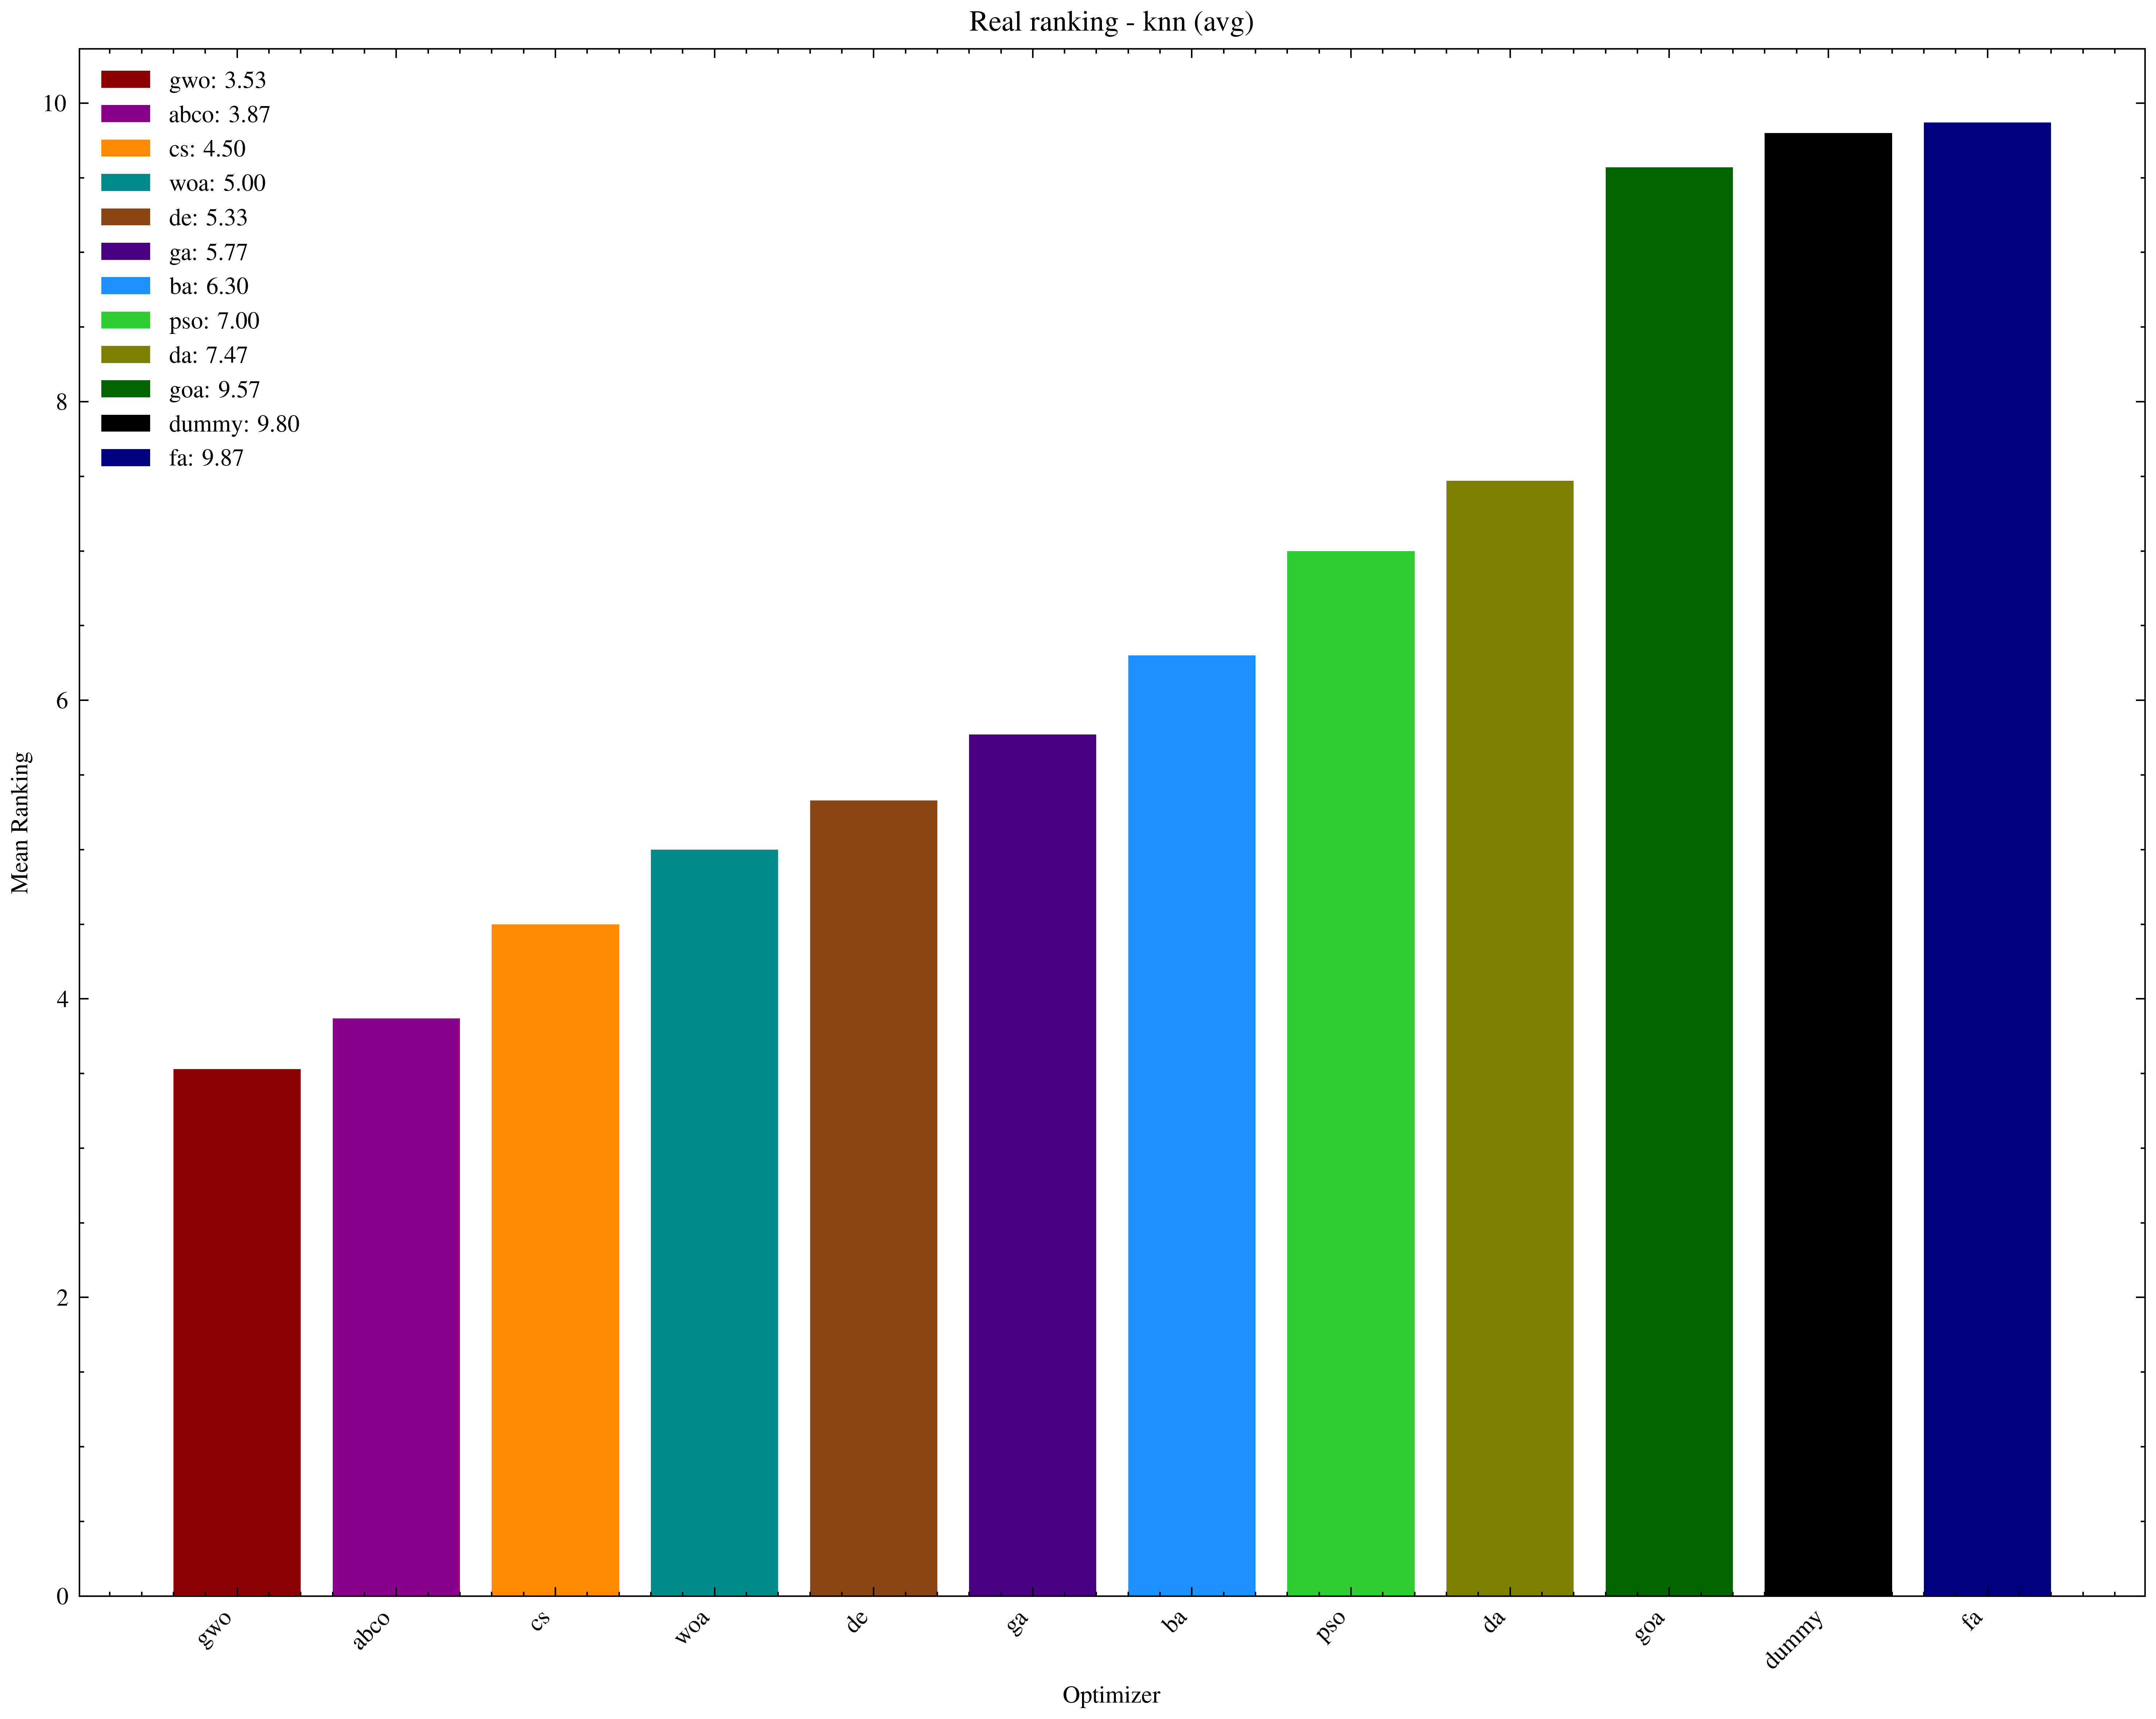
\includegraphics[width=\textwidth]{imagenes/fitness_charts/img/binary/rankings_knn_avg.png}
        \caption{Ranking por fitness para knn - binario}
        \label{fig:ranking_knn}
    \end{subfigure}
    \begin{subfigure}[b]{1\textwidth}
        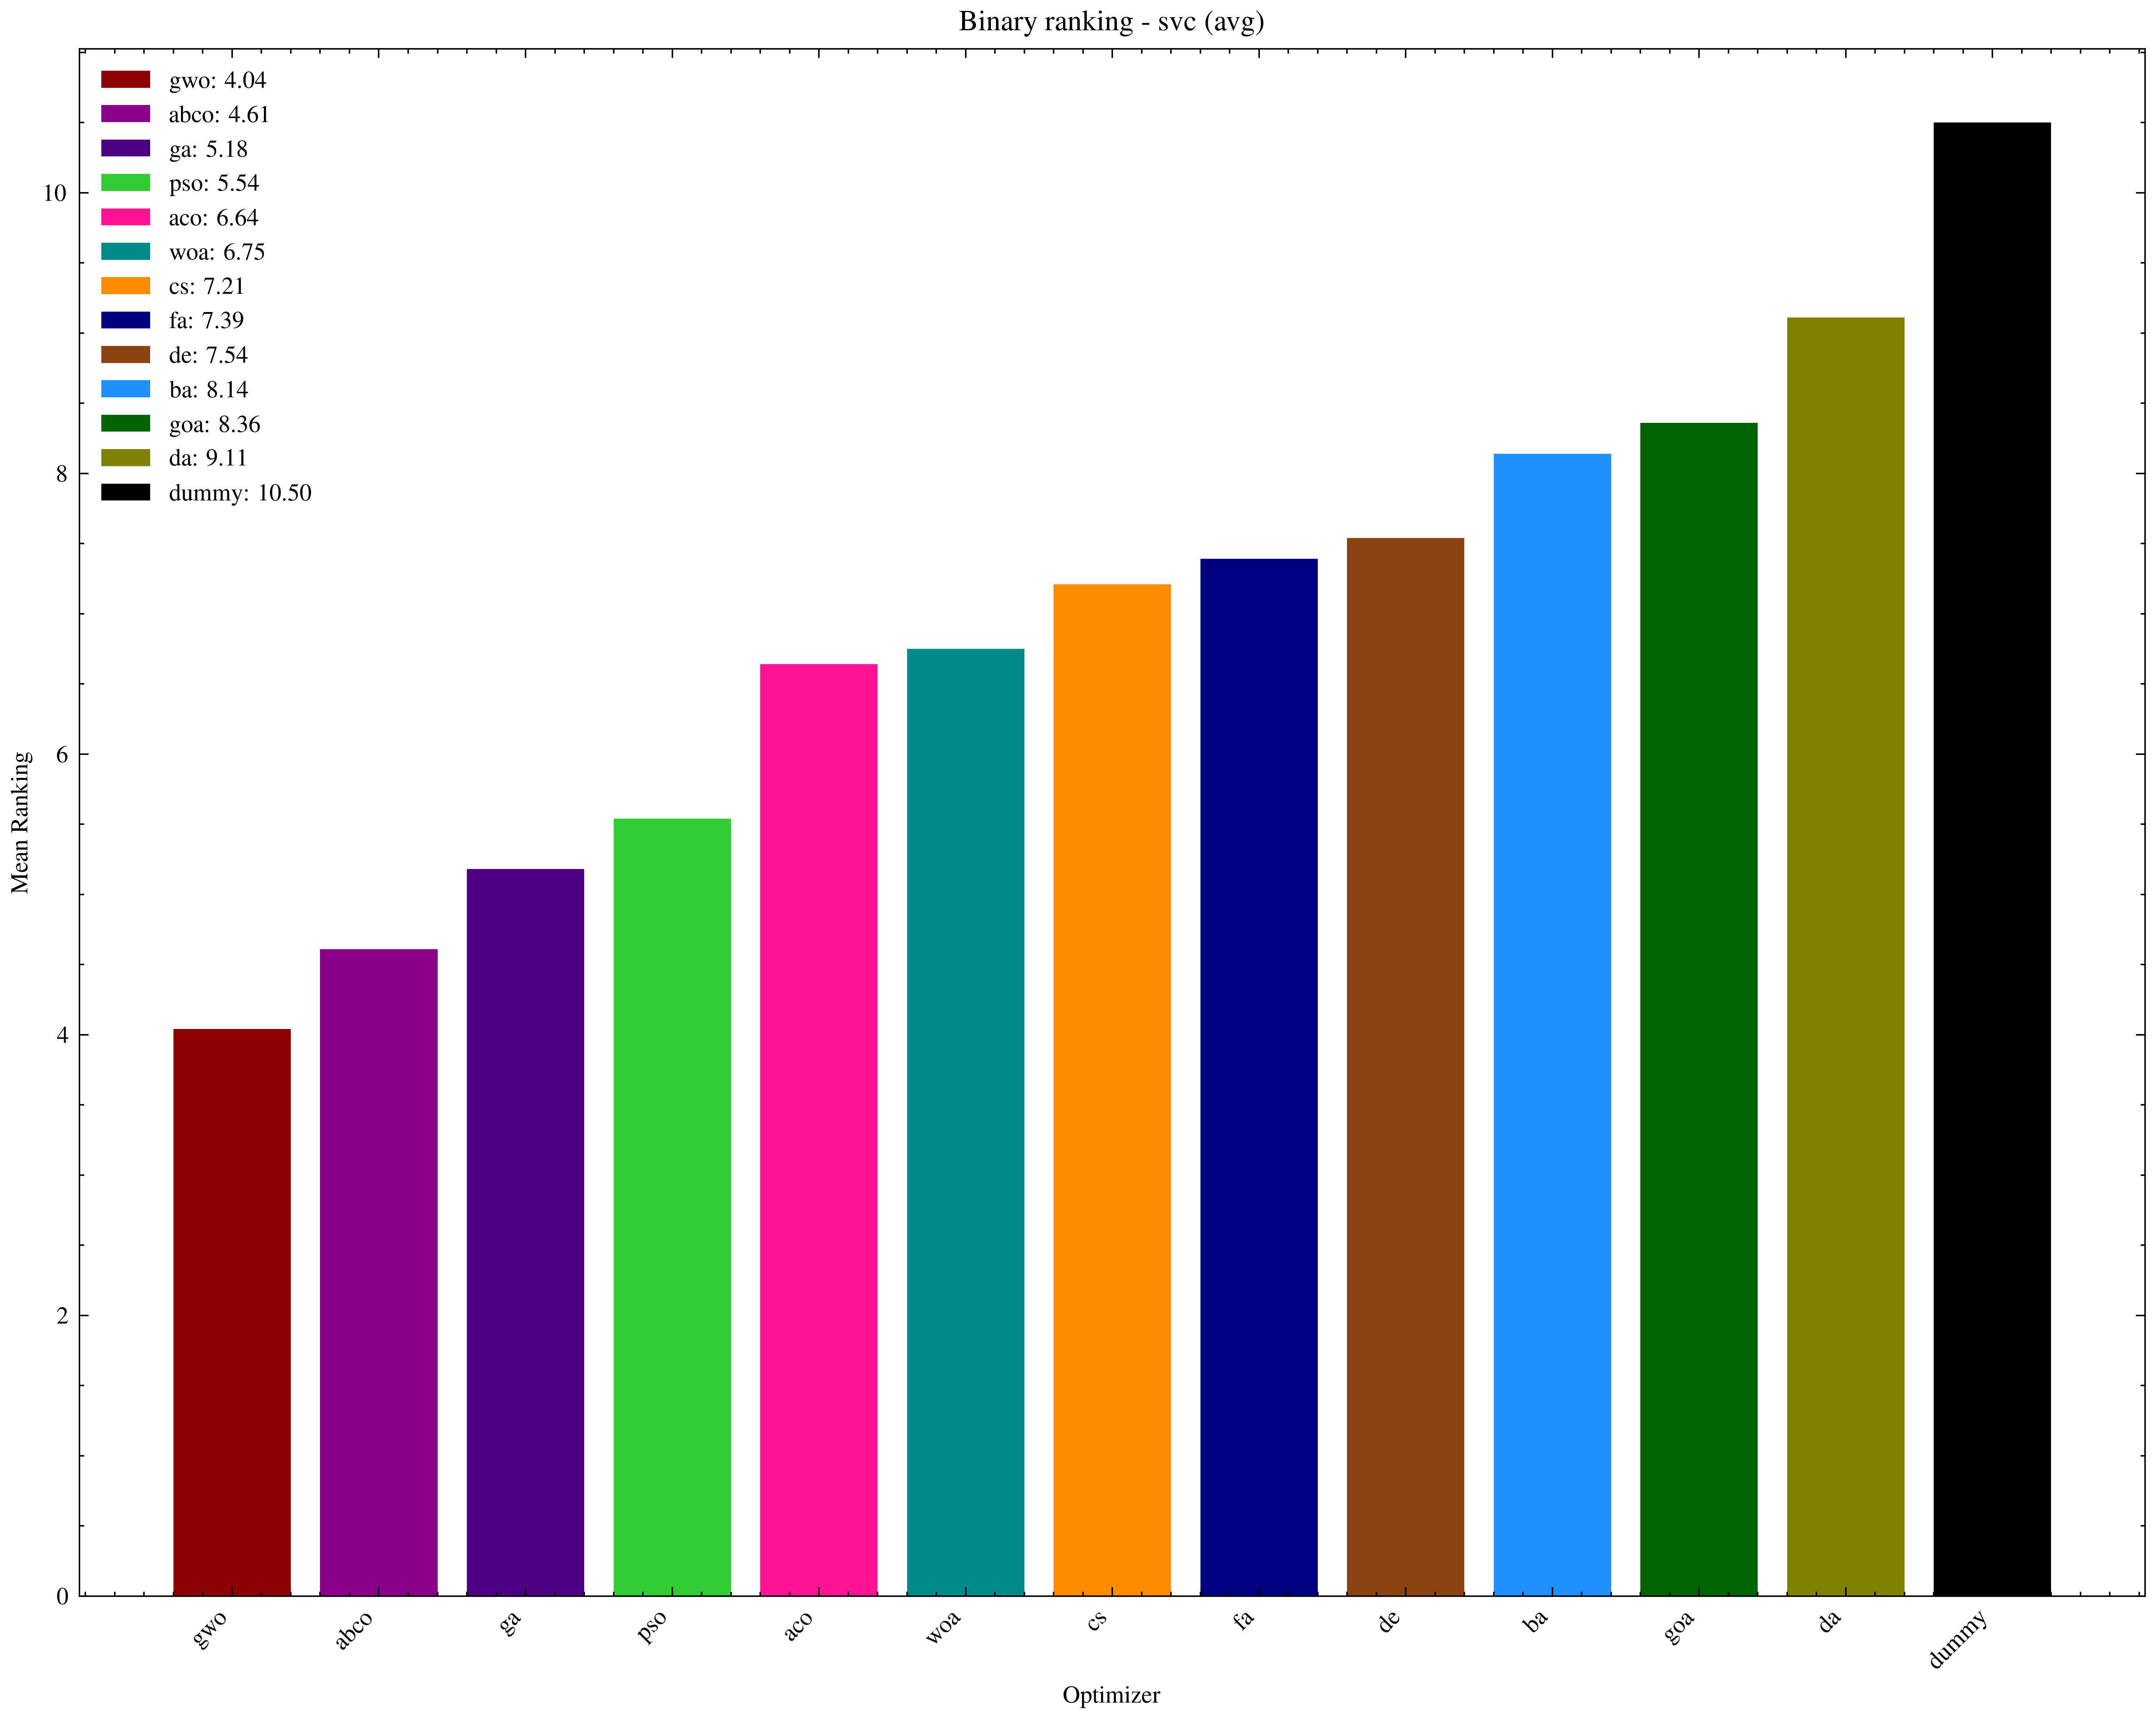
\includegraphics[width=\textwidth]{imagenes/fitness_charts/img/binary/rankings_svc_avg.png}
        \caption{Ranking por fitness para svc - binario}
        \label{fig:ranking_svc}
    \end{subfigure}
    \caption{Rankings para fitness - binario}
\end{figure}

Los rankings han sido creados basándose en los valores \textit{fitness} de los algoritmos para todos los conjuntos de datos. De forma visual es capaz de verse de un vistazo aquellos más versátiles, los que mejor se han comportado en distintos escenarios.\\[6pt]

En los rankings que se pueden observar en las gráficas \ref{fig:ranking_knn} para \textbf{kNN} y en \ref{fig:ranking_svc} para \textbf{SVC} puede verse como el mejor algoritmo es el \textbf{bGWO}, el algoritmo de los lobos grises, considerado como moderno. Puede observarse además el valor \textit{fitness} obtenido en las tablas \ref{tab:fitness_knn} y \ref{tab:fitness_svc}, con gran diferencia en comparación al resto. Le siguen algoritmos como \textbf{bPSO}, \textbf{bCS} y \textbf{bGA}.\\[6pt]

El \textbf{bPSO}, a pesar de ser uno de los algoritmos más antiguos en la optimización metaheurística, sigue manteniendo una posición destacada en los rankings. Estos hechos junto a su simplicidad y efectividad en la convergencia hacia soluciones óptimas, hacen ver que \textbf{bPSO} sigue siendo una opción muy interesante, incluso en problemas de tipo binario como la selección de características, escenario para los que \textbf{bPSO} no fue diseñado. Esto hace de esta metaheurística una opción que parece sugerir mucha robustez.\\[6pt]

El \textbf{CS}, basado en el comportamiento de anidación de ciertos pájaros, también se muestra como una opción fuerte, compitiendo por el podio con \textbf{bGA}.\\[6pt]

Finalmente, el \textbf{bGA}, uno de los algoritmos más estudiados y aplicados en el ámbito de la optimización, sigue siendo relevante. Su capacidad para encontrar soluciones óptimas a través de mecanismos inspirados en la evolución natural, como la selección, el cruce y la mutación, le permite abordar una amplia gama de problemas con éxito. Además, este algoritmo al ser inicialmente pensado para aplicarse en dominios de codificación discreta, hace de esta metaheurística una opción muy interesante y robusta en el problema de selección de características, además de llevar años siendo aplicado con éxito en otros dominios.\\[6pt]

Es visible que algunas de estas nuevas propuestas son muy potentes, llegando a mejorar en la propuesta binaria en comparación a algoritmos clásicos que llevan tiempo en la escena como las opciones \textit{de facto}. Pese a ello, el grueso de los algoritmos comparados son opciones modernas, y muchos de estos algoritmos clásicos obtienen mejores resultados que la mayoría de este reciente grupo. De las cinto mejores, tres de ellos son clásicos, lo cual es más impresionante si se considera que hay un desbalance en número de \textit{clásicos vs modernos}. \textit{DE} es otro algoritmo asentado, que es capaz de clasificar en posiciones medias de \textit{fitness}.\\[6pt]

El peor de todos los algoritmos comparados es, sin embargo, \textbf{bABCO}, un algoritmo clásico. No parece poder alcanzar en calidad ni a modernos ni a algoritmos más antiguos como \textbf{PSO}.

\subsubsection{Mejor vs Peor}
Como ya se ha podido observar en, el algoritmo con mejor puntuación es \textbf{bGWO} y el peor \textbf{bABCO} (\ref{tab:fitness_svc}, \ref{tab:fitness_knn}, \ref{tab:ranking_fitness_bin}). \\[6pt]
En las figuras de \ref{fig:convergencia_svc_2} y \ref{fig:convergencia_svc_1} se aprecia como \textbf{bABCO} muestra rendimientos muy buenos en según que conjunto de datos. Por ejemplo, en \textit{yeast} o en \textit{sonar}, el algoritmo obtiene resultados muy decentes y competitivos siendo estos dos conjuntos de datos de los más complicados de la selección, por convergencia y número de características. Pese a ello, en conjunto, no consigue superar al resto.\\[6pt]
En cambio \textbf{bGWO} parece un adaptarse bien a todos los problemas seleccionados sin excepción. Es capaz de obtener el mínimo, en el valor \textit{fitness} de evaluación durante el entrenamiento, en casi todos los \textit{datasets}.

\begin{table}[htb]
    \centering
    \begin{tabular}{lllll}
        \toprule
        {}         & Original  & Holm           & Hommel         & Hochberg       \\
        \midrule
        dummy\_knn & 6.104E-05 & \textbf{0.002} & \textbf{0.002} & \textbf{0.002} \\
        dummy\_svc & 3.052E-04 & \textbf{0.007} & \textbf{0.007} & \textbf{0.007} \\
        goa\_knn   & 0.001     & \textbf{0.027} & \textbf{0.024} & \textbf{0.027} \\
        abco\_knn  & 0.002     & \textbf{0.034} & \textbf{0.032} & \textbf{0.034} \\
        abco\_svc  & 0.002     & \textbf{0.045} & \textbf{0.043} & \textbf{0.045} \\
        ba\_svc    & 0.004     & 0.085          & 0.078          & 0.085          \\
        da\_svc    & 0.005     & 0.102          & 0.097          & 0.102          \\
        goa\_svc   & 0.008     & 0.149          & 0.149          & 0.149          \\
        de\_knn    & 0.026     & 0.435          & 0.307          & 0.409          \\
        aco\_knn   & 0.026     & 0.435          & 0.307          & 0.409          \\
        da\_knn    & 0.064     & 0.956          & 0.573          & 0.887          \\
        woa\_svc   & 0.073     & 1.000          & 0.588          & 0.887          \\
        fa\_knn    & 0.083     & 1.000          & 0.653          & 0.887          \\
        ga\_knn    & 0.107     & 1.000          & 0.686          & 0.887          \\
        cs\_knn    & 0.107     & 1.000          & 0.686          & 0.887          \\
        de\_svc    & 0.109     & 1.000          & 0.686          & 0.887          \\
        fa\_svc    & 0.121     & 1.000          & 0.719          & 0.887          \\
        ba\_knn    & 0.135     & 1.000          & 0.719          & 0.887          \\
        ga\_svc    & 0.252     & 1.000          & 0.799          & 0.887          \\
        woa\_knn   & 0.256     & 1.000          & 0.799          & 0.887          \\
        cs\_svc    & 0.364     & 1.000          & 0.887          & 0.887          \\
        pso\_knn   & 0.489     & 1.000          & 0.887          & 0.887          \\
        aco\_svc   & 0.490     & 1.000          & 0.887          & 0.887          \\
        pso\_svc   & 0.599     & 1.000          & 0.887          & 0.887          \\
        gwo\_knn   & 0.887     & 1.000          & 0.887          & 0.887          \\
        \bottomrule
    \end{tabular}
    \caption{P-valores del mejor vs el resto - binario}
    \label{tab:p-valus_gwo_vs_rest}
\end{table}

Se procede a hacer una comparativa estadística mediante la prueba de \textit{Wilcoxon} y el test post hoc de \textit{Holm} para determinar las diferencias significativas entre el mejor algoritmo (\textbf{bGWO}) y el resto. Los resultados, presentados en la tabla \ref{tab:p-valus_gwo_vs_rest}, muestran los p-valores originales y ajustados, lo que nos permite identificar cuáles de las diferencias observadas son estadísticamente significativas con un error corregido. Este análisis es crucial para validar los resultados y asegurar que las conclusiones obtenidas no sean producto del azar, proporcionando una base sólida para afirmar la superioridad de \textbf{bGWO} frente a los demás algoritmos en los conjuntos de datos evaluados, en frente al peor de ellos.\\[6pt]

Para evaluar el rendimiento de los algoritmos, se plantean las siguientes hipótesis:

\textbf{Hipótesis nula (\(H_0\))}:
\begin{equation}
    H_0: \text{Rendimiento}_{bGWO} \leq \text{Rendimiento}_{\text{bABCO}}
\end{equation}

\textbf{Hipótesis alternativa (\(H_1\))}:
\begin{equation}
    H_1: \text{Rendimiento}_{bGWO} > \text{Rendimiento}_{\text{bABCO}}
\end{equation}

Si bien no se observan diferencias significativas sobre la mayoría de algoritmos, sí sobre el peor (\textbf{bABCO}) y sobre la versión de \textbf{bGOA} usando \textbf{kNN}. Tanto en la versión que utiliza el clasificador \textbf{SVC} como en \textbf{kNN} se obtienen resultados suficientemente significativos como para poder considerar que los resultados de \textbf{bGWO} frente a los de \textbf{bABCO} no son producto del azar. Por tanto, utilizando un valor crítico de $\alpha=0.05$ se puede rechazar la hipótesis nula.


\begin{figure}[htb]
    \centering
    \begin{subfigure}[b]{0.45\textwidth}
        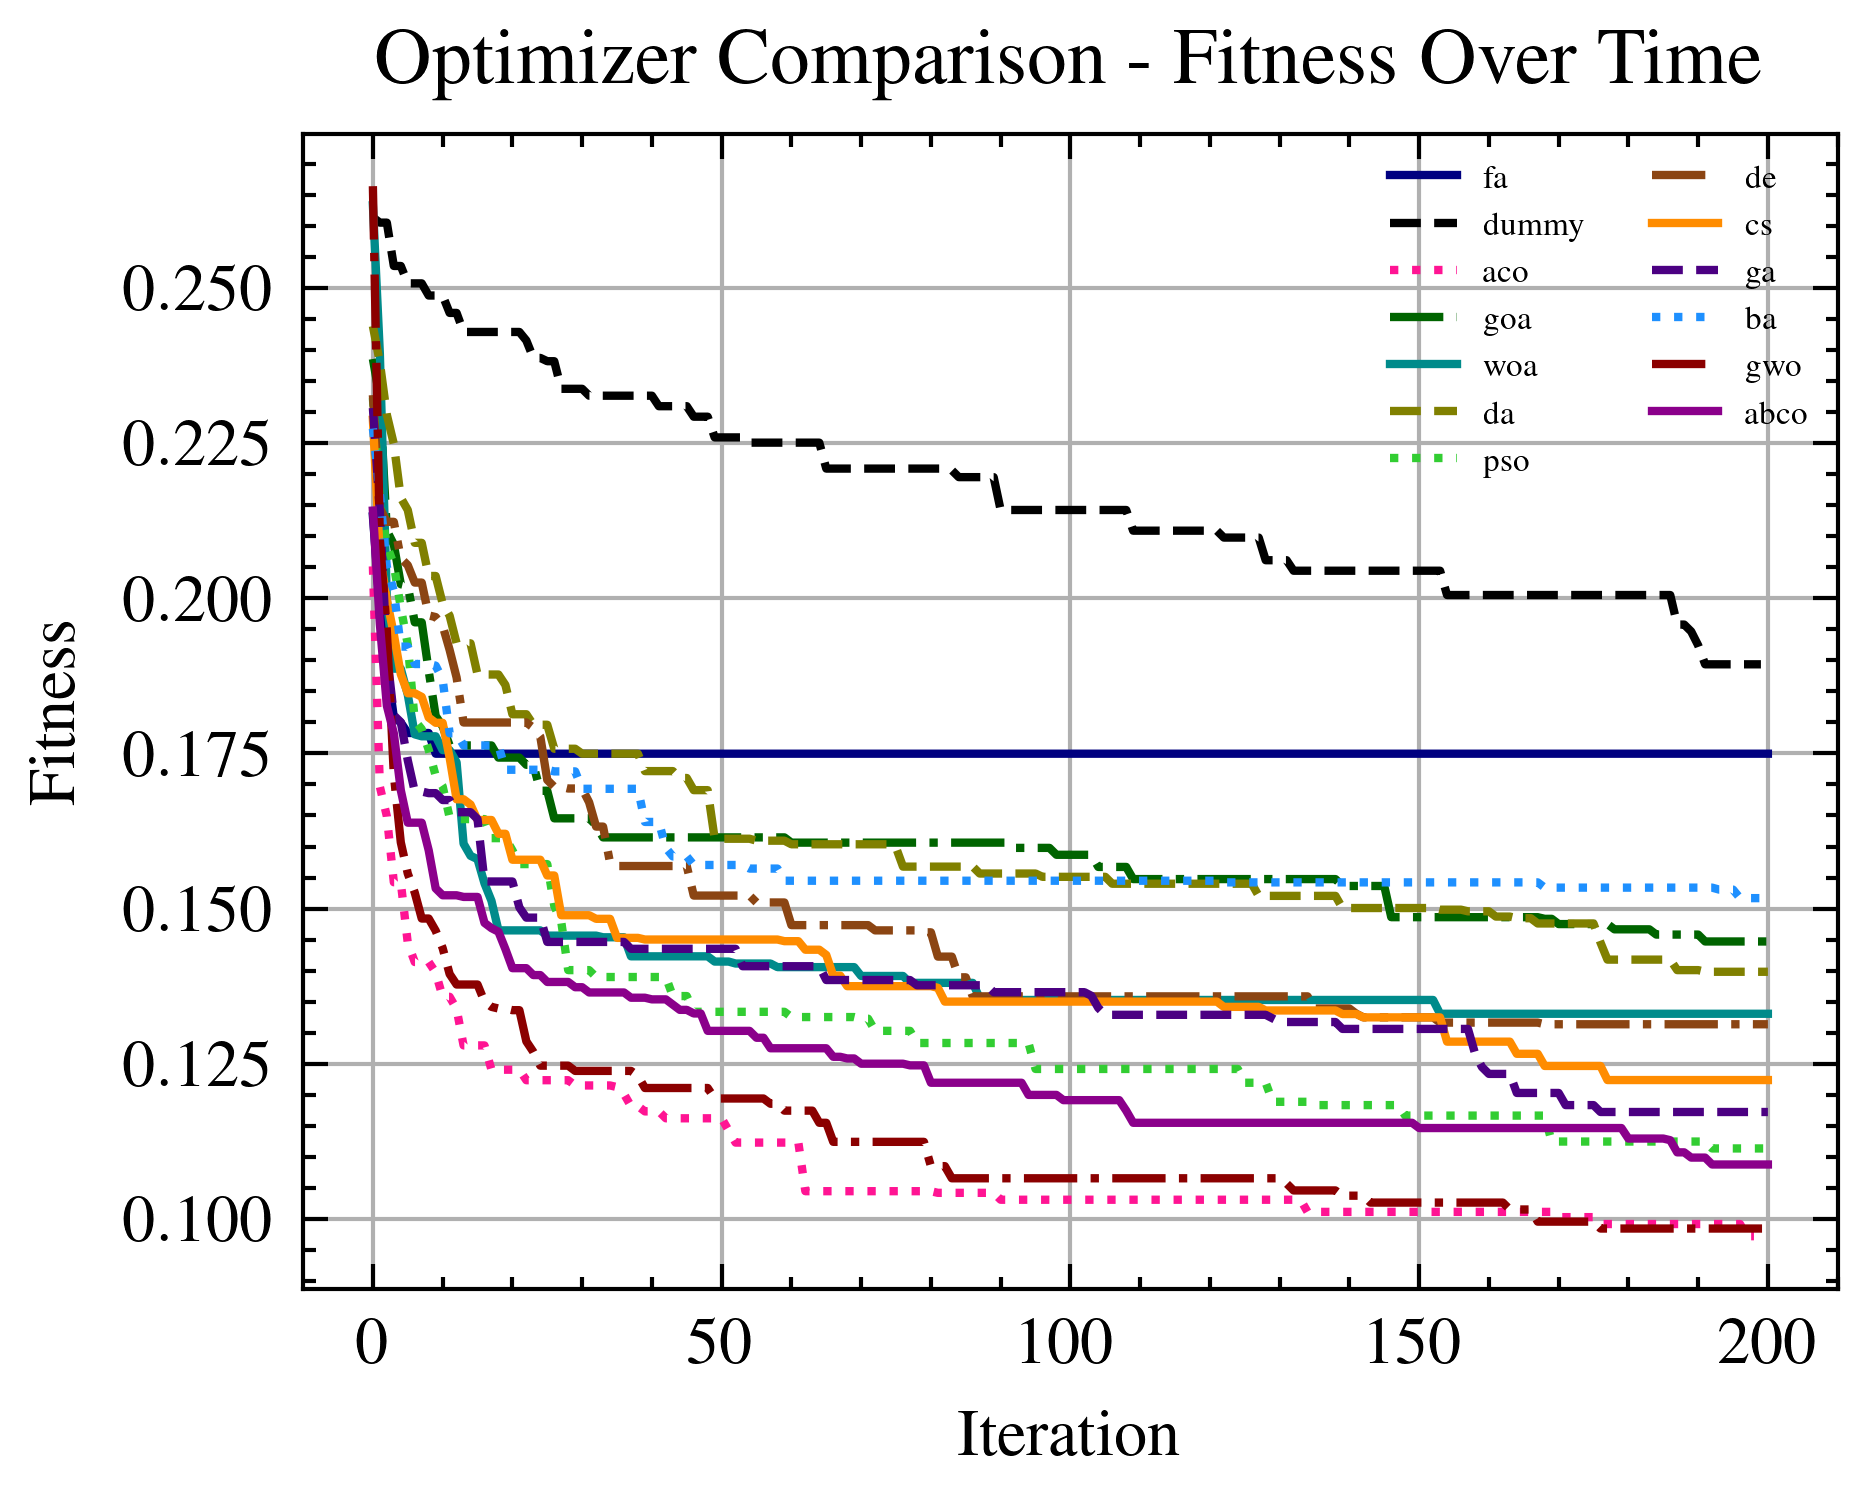
\includegraphics[width=\textwidth]{imagenes/fitness_charts/img/binary/breast-cancer/optimizers_fitness_svc.png}
        \caption{breast-cancer}
        \label{fig:convergencia_breast_cancer_svc}
    \end{subfigure}
    \begin{subfigure}[b]{0.45\textwidth}
        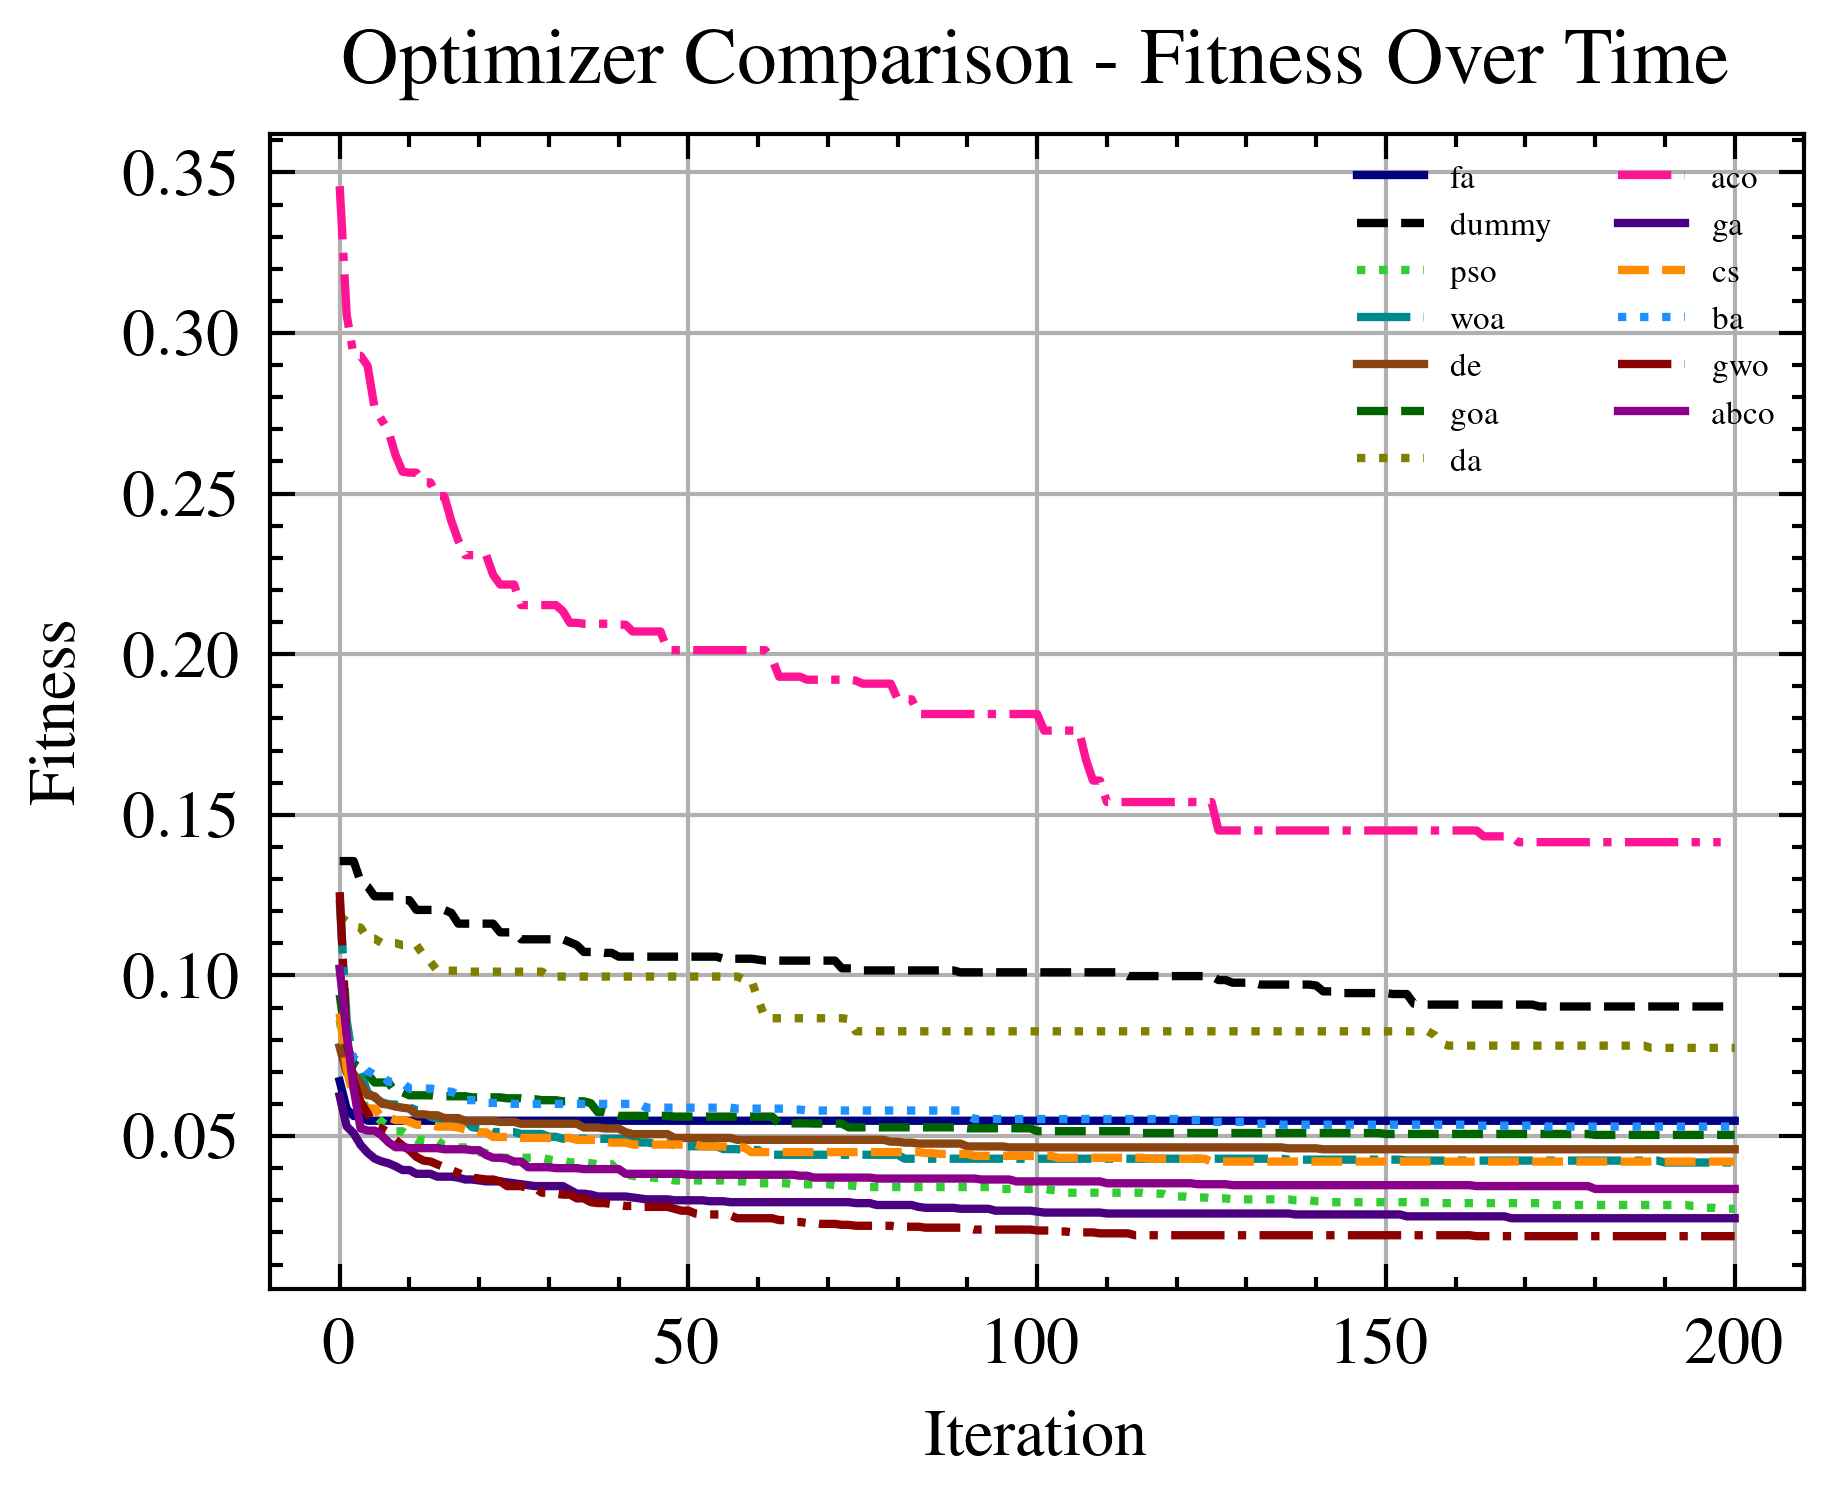
\includegraphics[width=\textwidth]{imagenes/fitness_charts/img/binary/dermatology/optimizers_fitness_svc.png}
        \caption{dermatology}
        \label{fig:convergencia_dermatology_svc}
    \end{subfigure}

    \begin{subfigure}[b]{0.45\textwidth}
        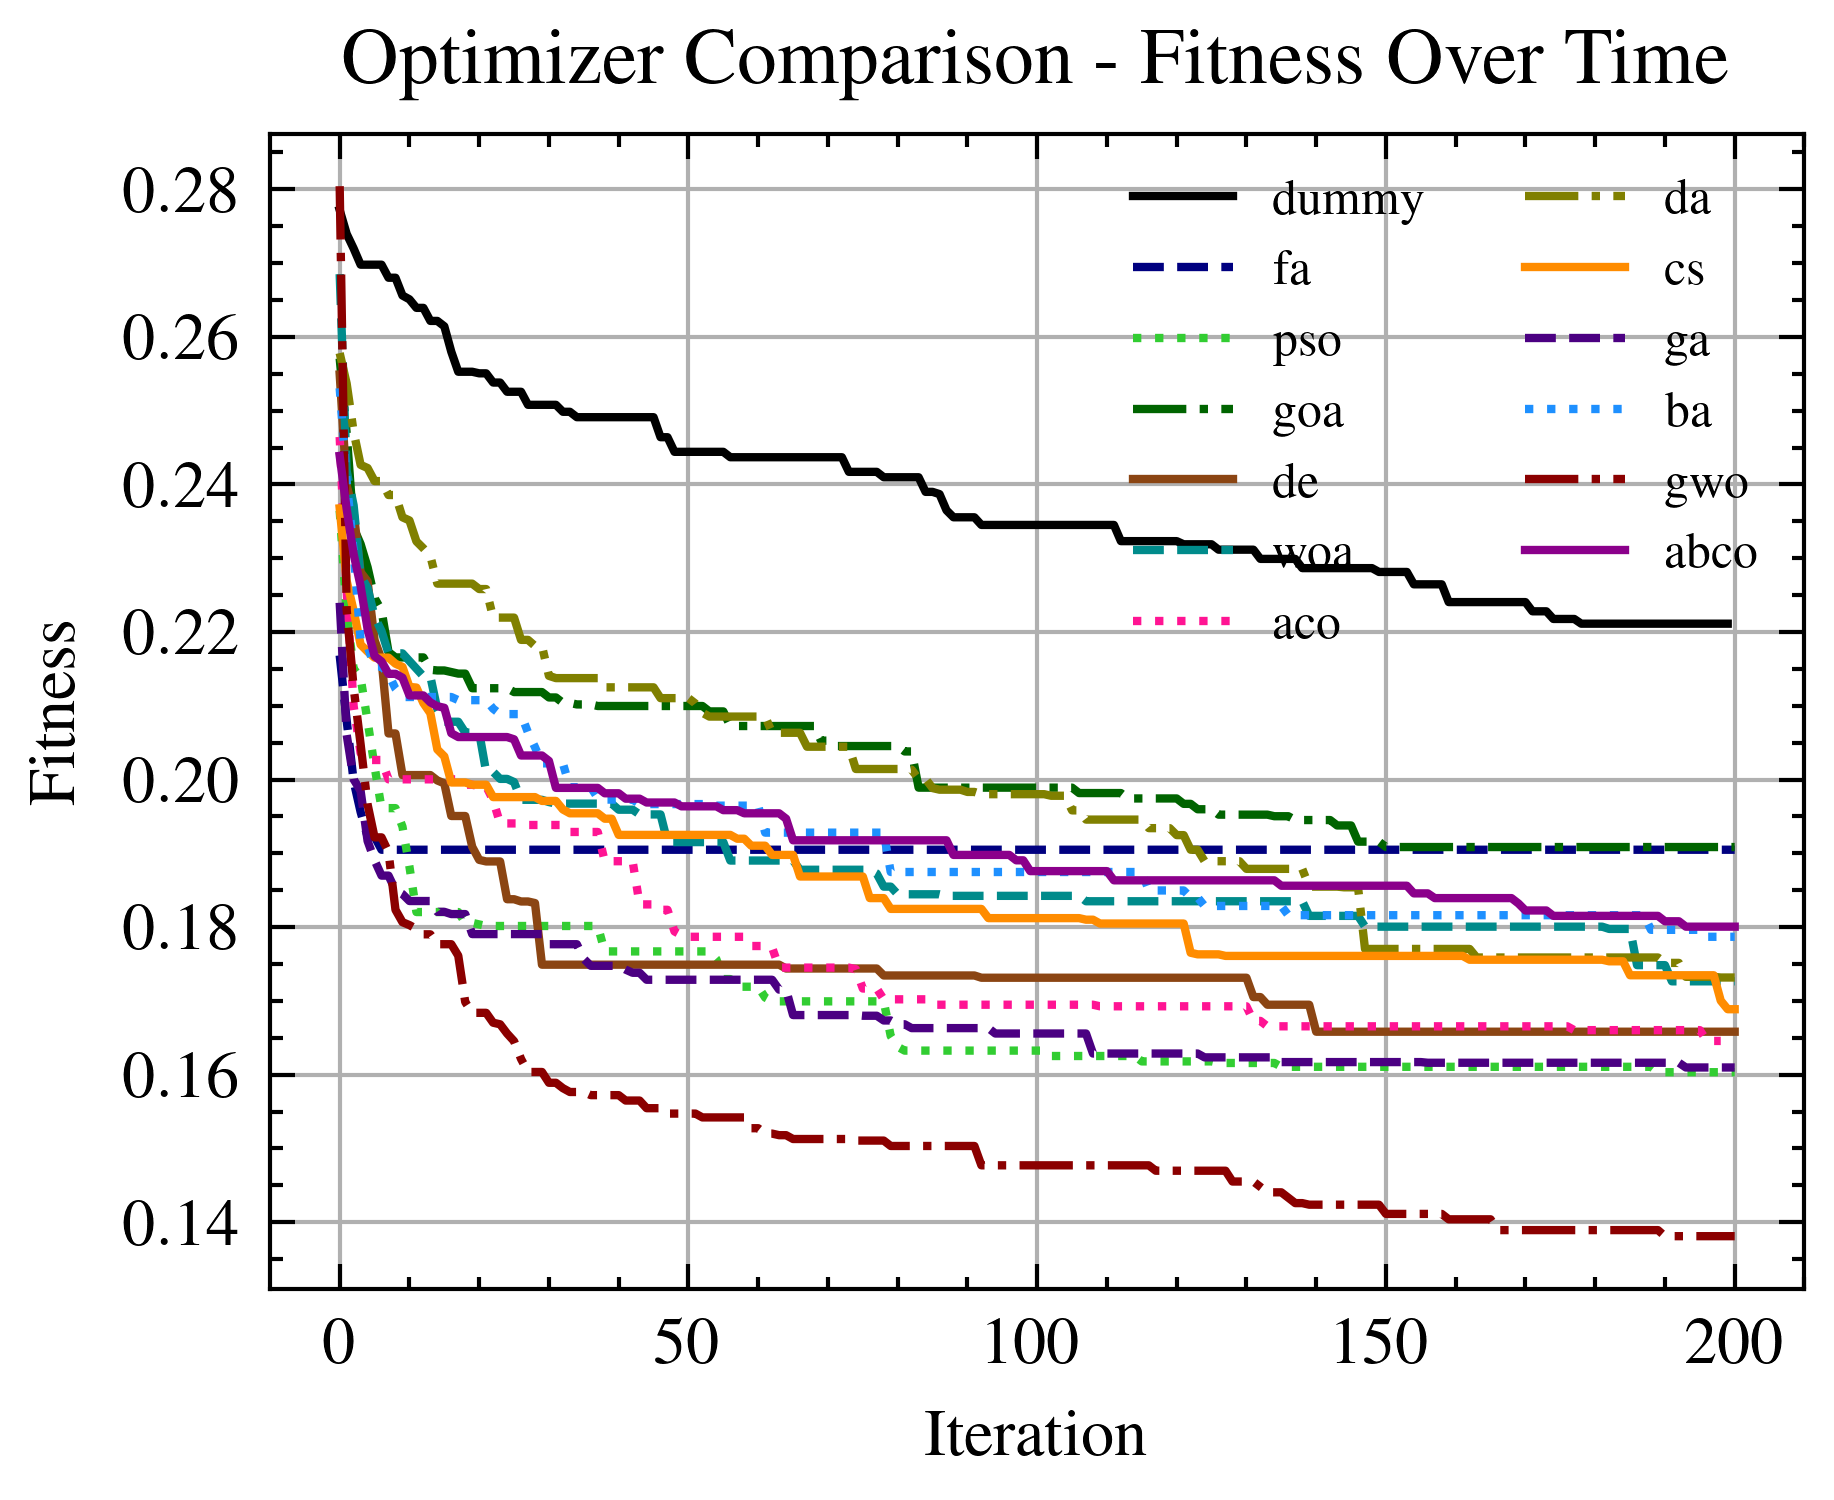
\includegraphics[width=\textwidth]{imagenes/fitness_charts/img/binary/diabetes/optimizers_fitness_svc.png}
        \caption{diabetes}
        \label{fig:convergencia_diabetes_svc}
    \end{subfigure}
    \begin{subfigure}[b]{0.45\textwidth}
        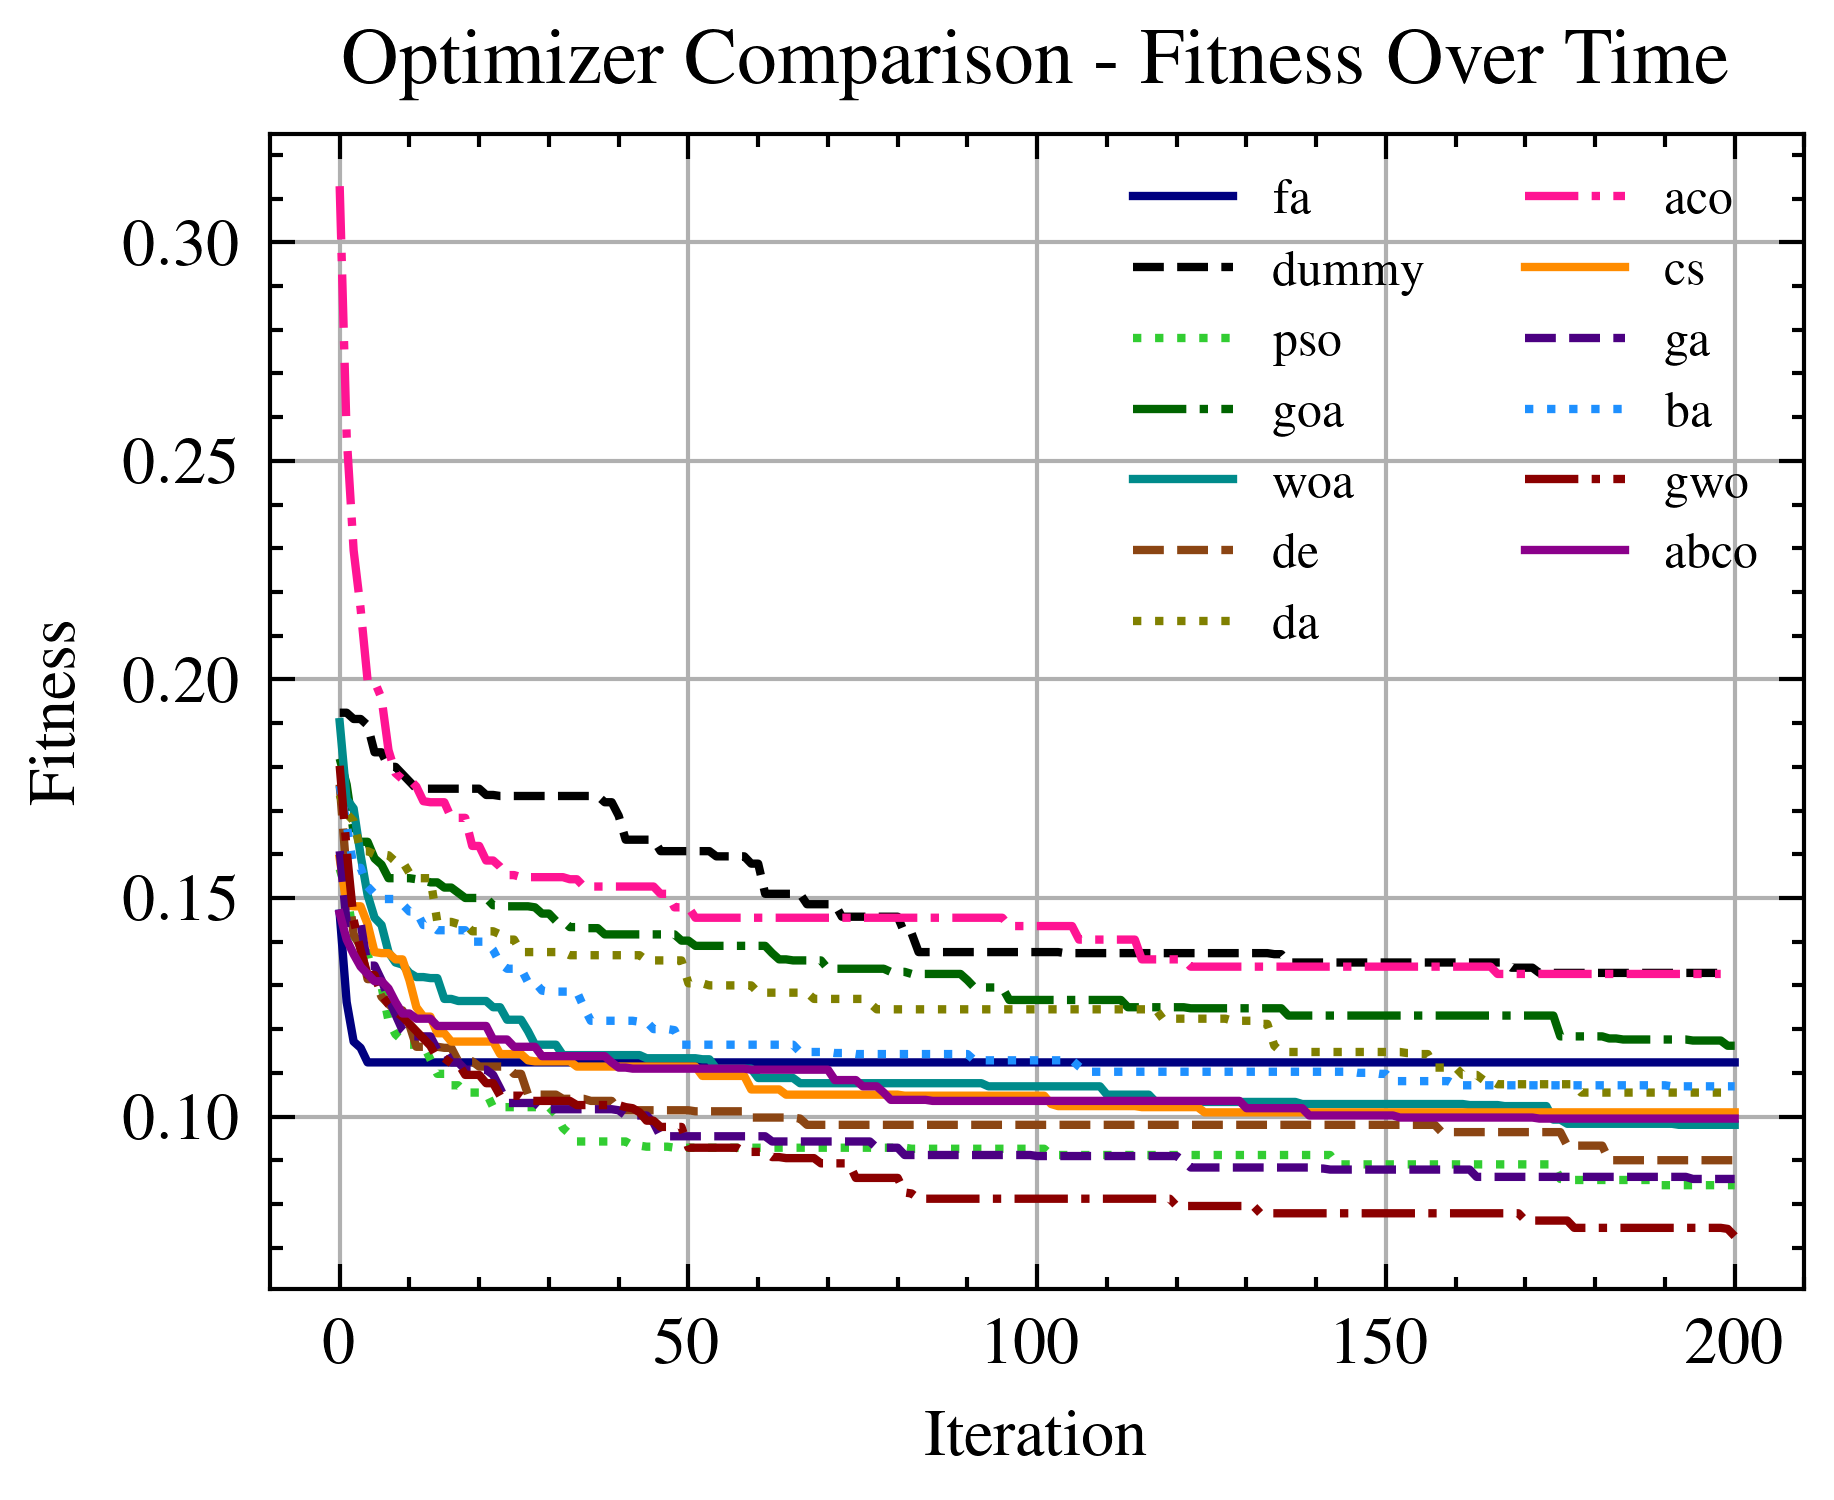
\includegraphics[width=\textwidth]{imagenes/fitness_charts/img/binary/ecoli/optimizers_fitness_svc.png}
        \caption{ecoli}
        \label{fig:convergencia_ecoli_svc}
    \end{subfigure}

    \begin{subfigure}[b]{0.45\textwidth}
        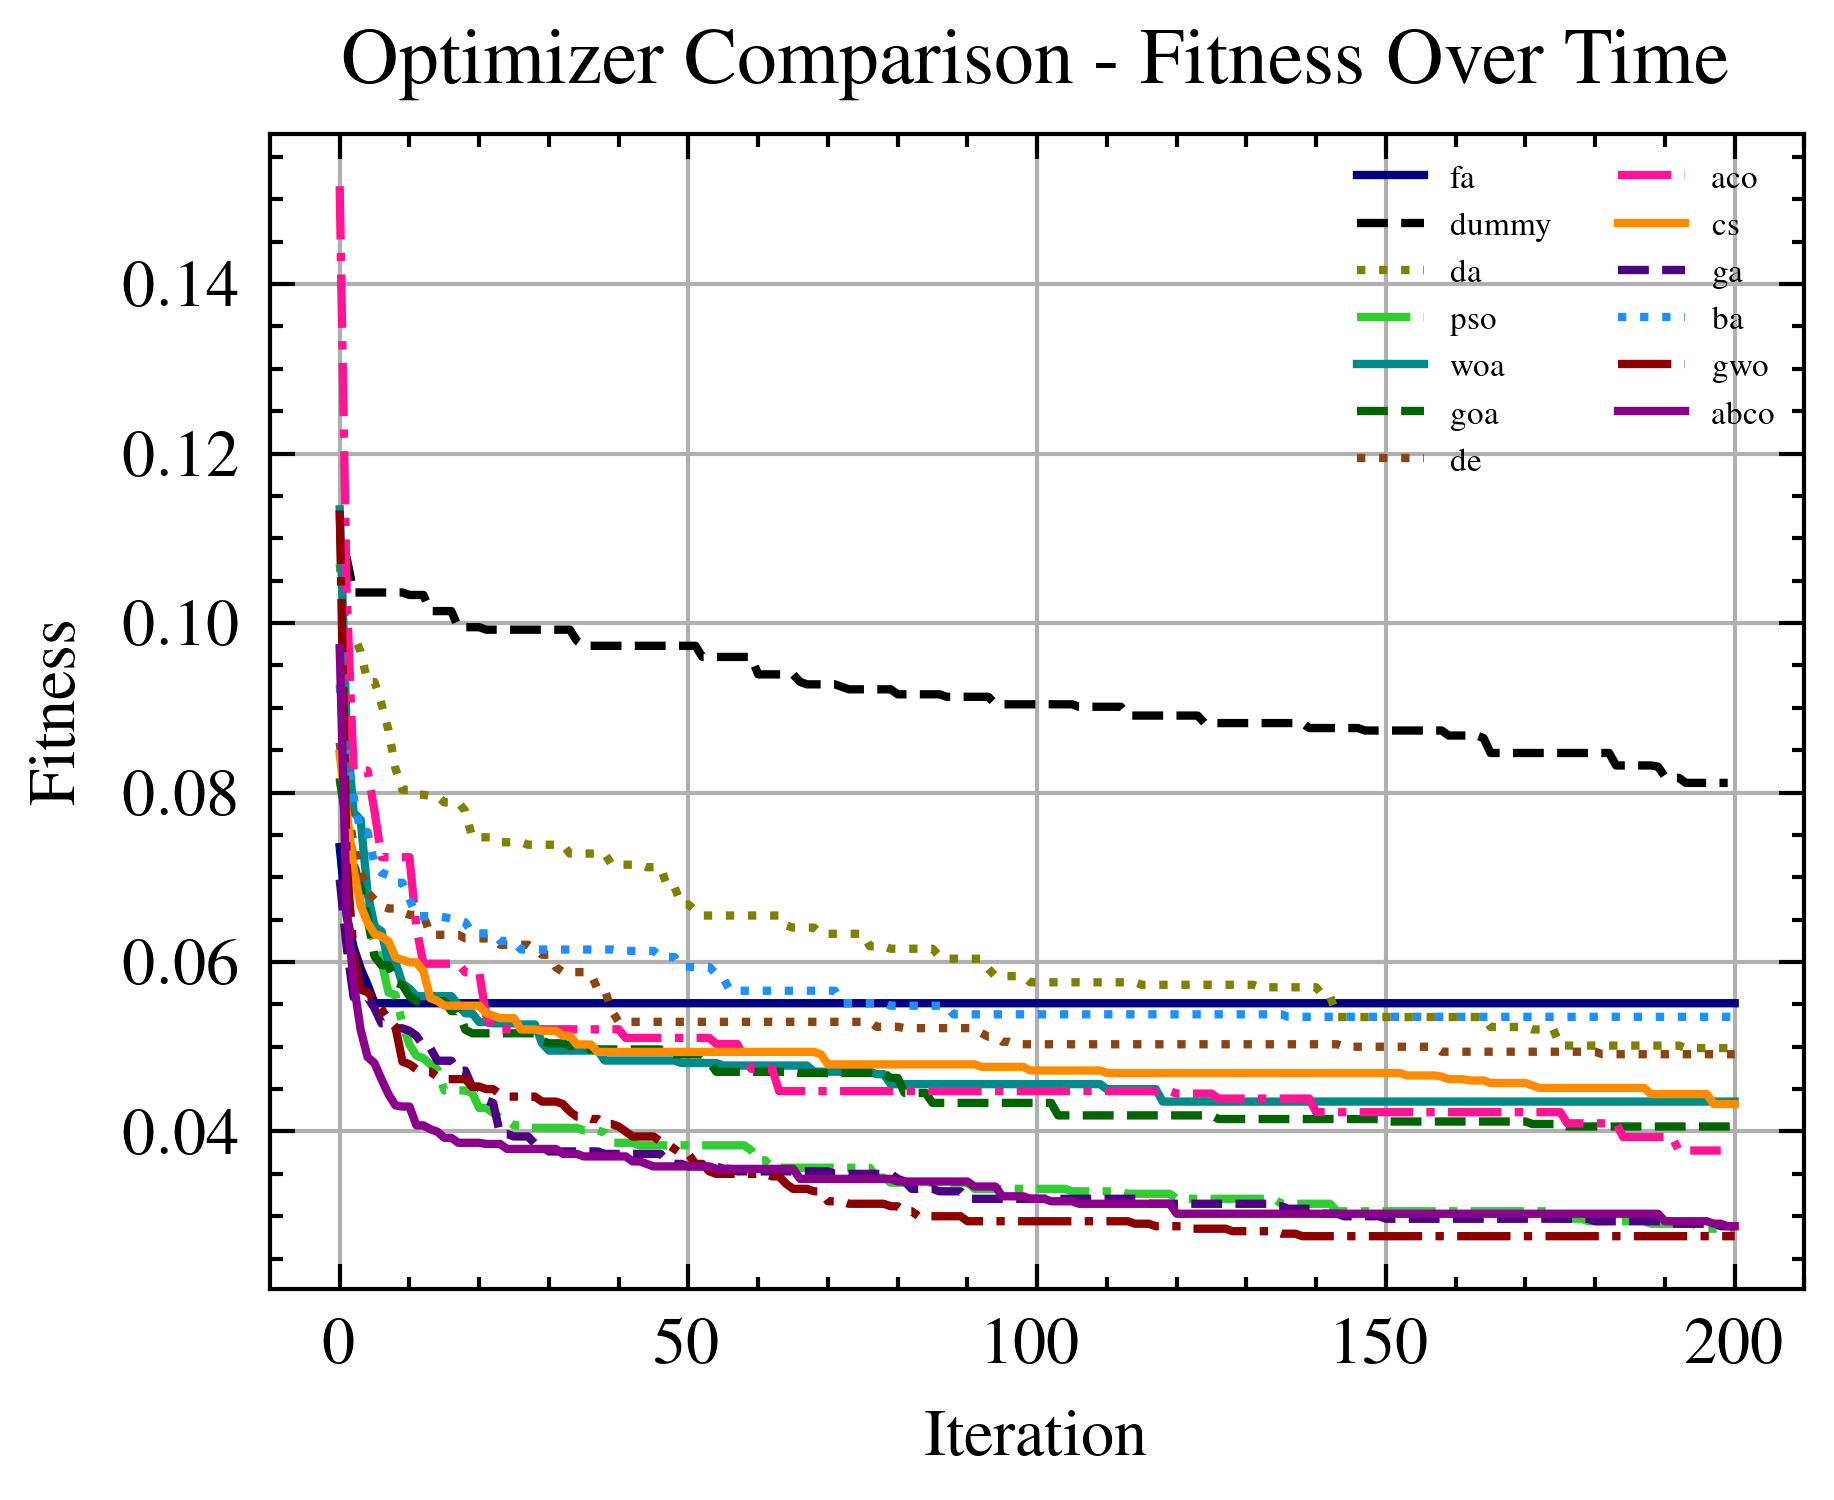
\includegraphics[width=\textwidth]{imagenes/fitness_charts/img/binary/ionosphere/optimizers_fitness_svc.png}
        \caption{ionosphere}
        \label{fig:convergencia_ionosphere_svc}
    \end{subfigure}
    \begin{subfigure}[b]{0.45\textwidth}
        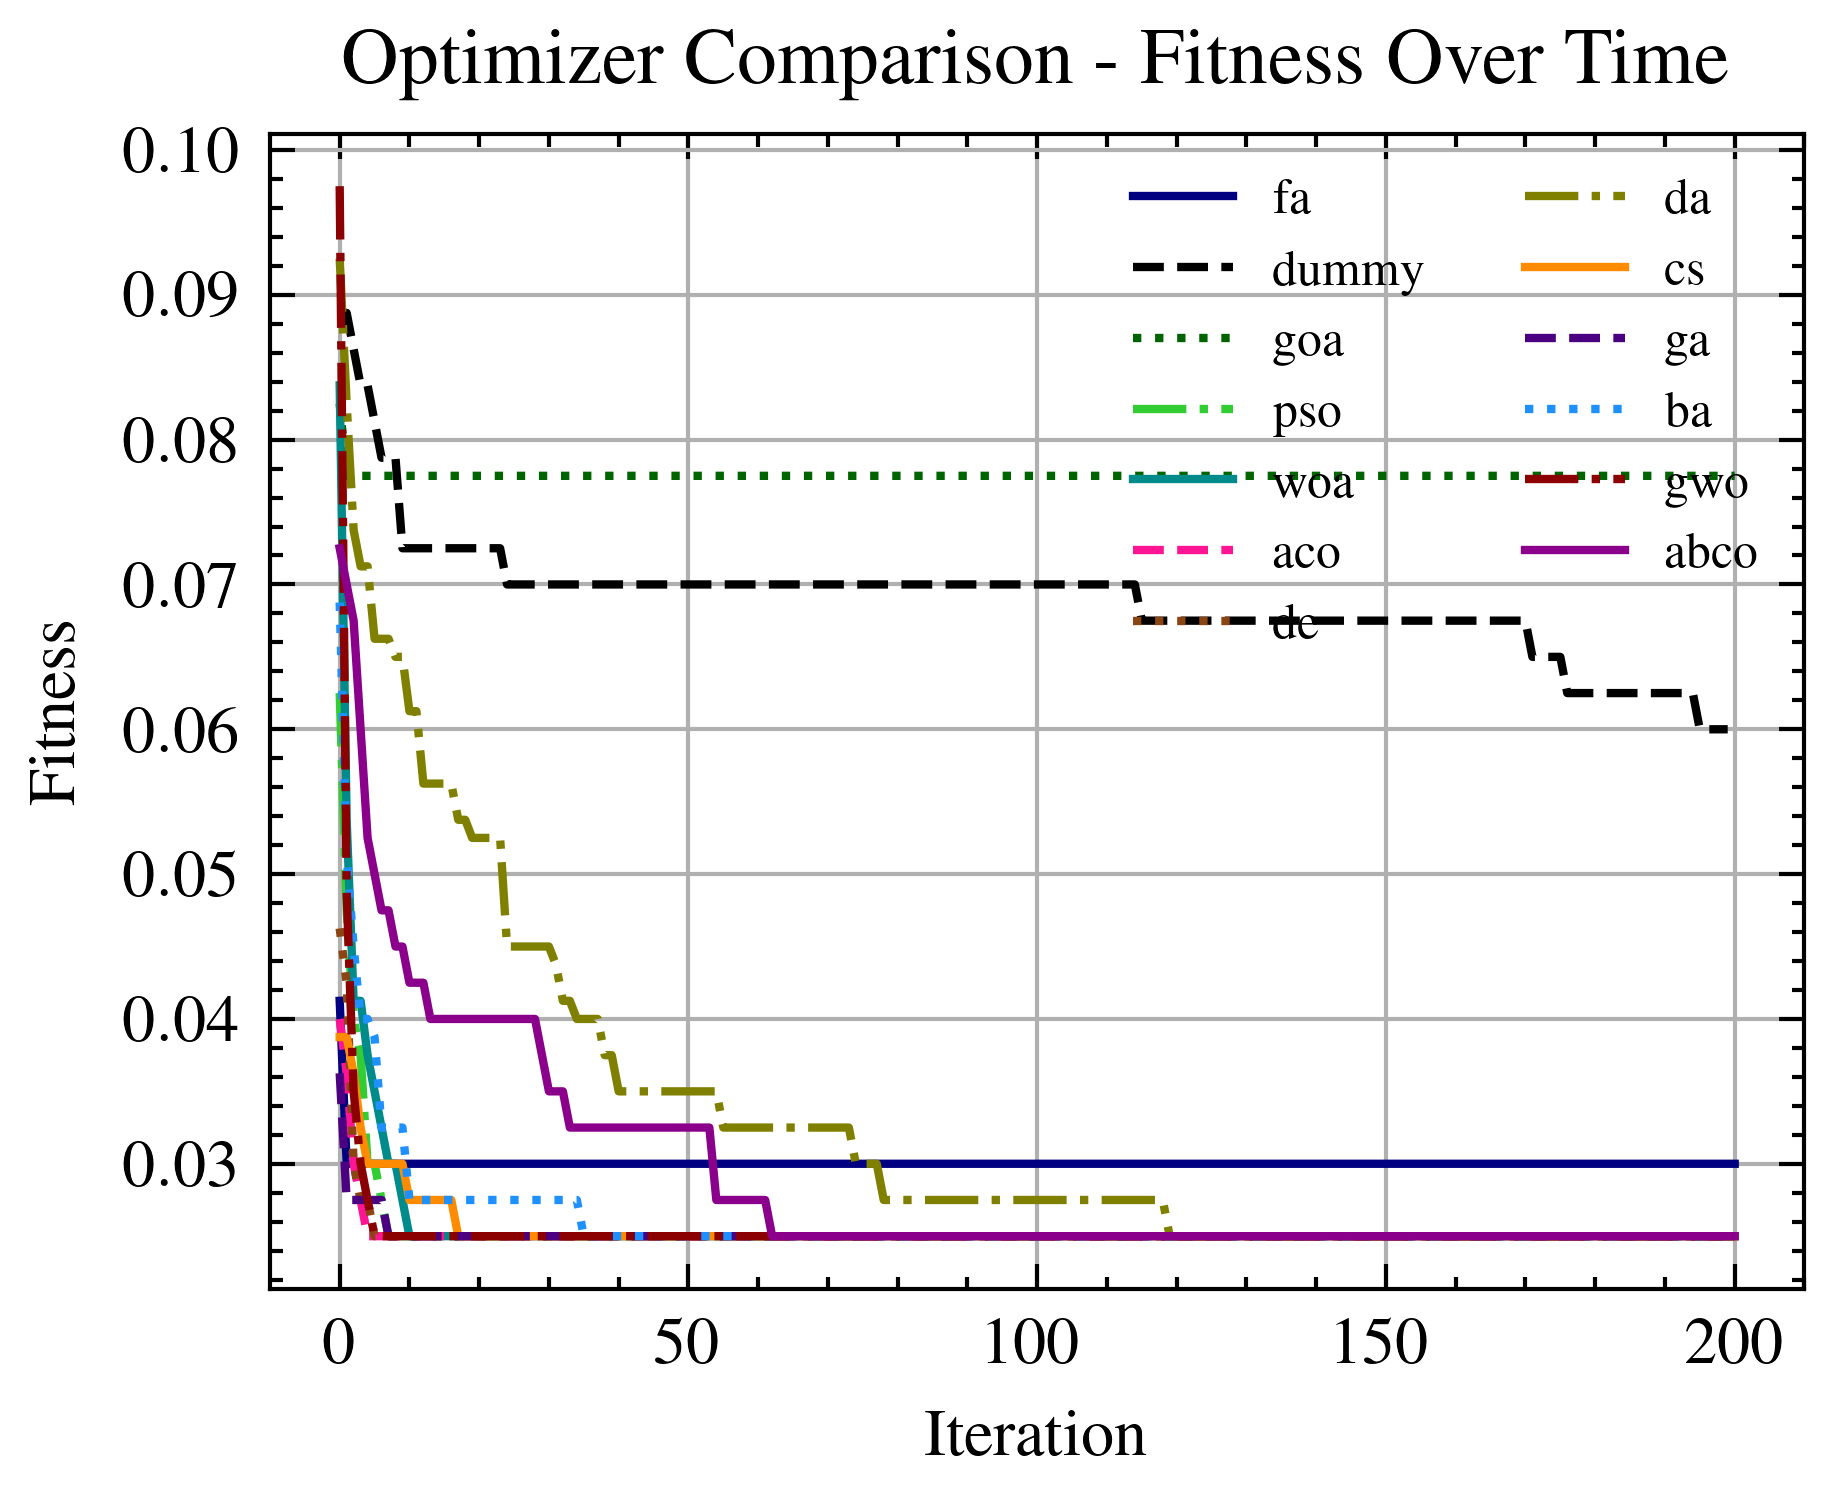
\includegraphics[width=\textwidth]{imagenes/fitness_charts/img/binary/iris/optimizers_fitness_svc.png}
        \caption{iris}
        \label{fig:convergencia_iris_svc}
    \end{subfigure}

    \begin{subfigure}[b]{0.45\textwidth}
        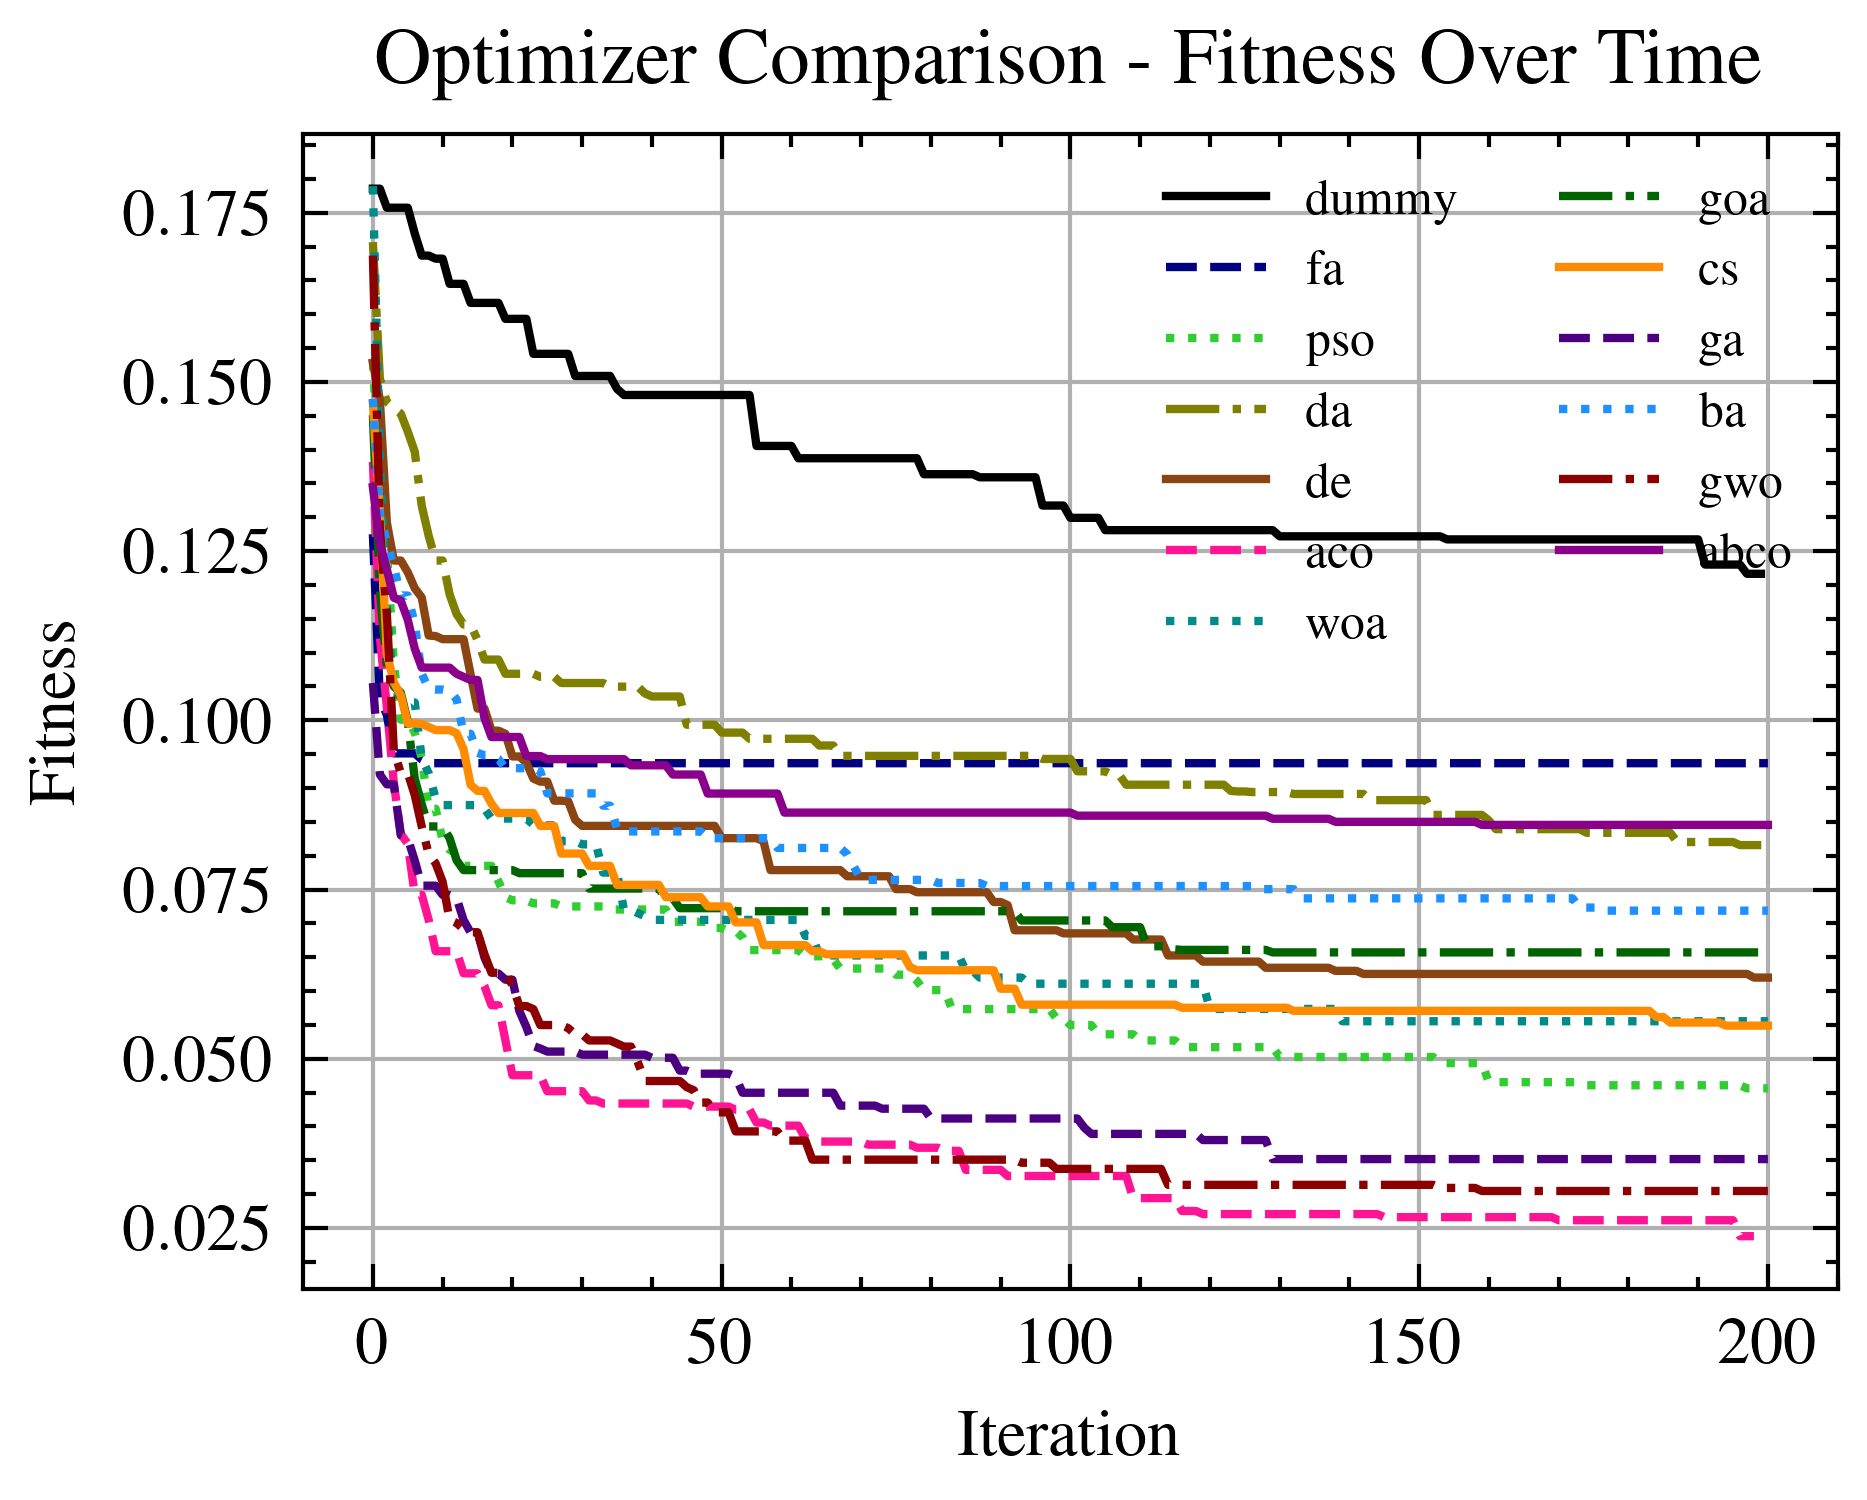
\includegraphics[width=\textwidth]{imagenes/fitness_charts/img/binary/parkinsons/optimizers_fitness_svc.png}
        \caption{parkinsons}
        \label{fig:convergencia_parkinsons_svc}
    \end{subfigure}
    \begin{subfigure}[b]{0.45\textwidth}
        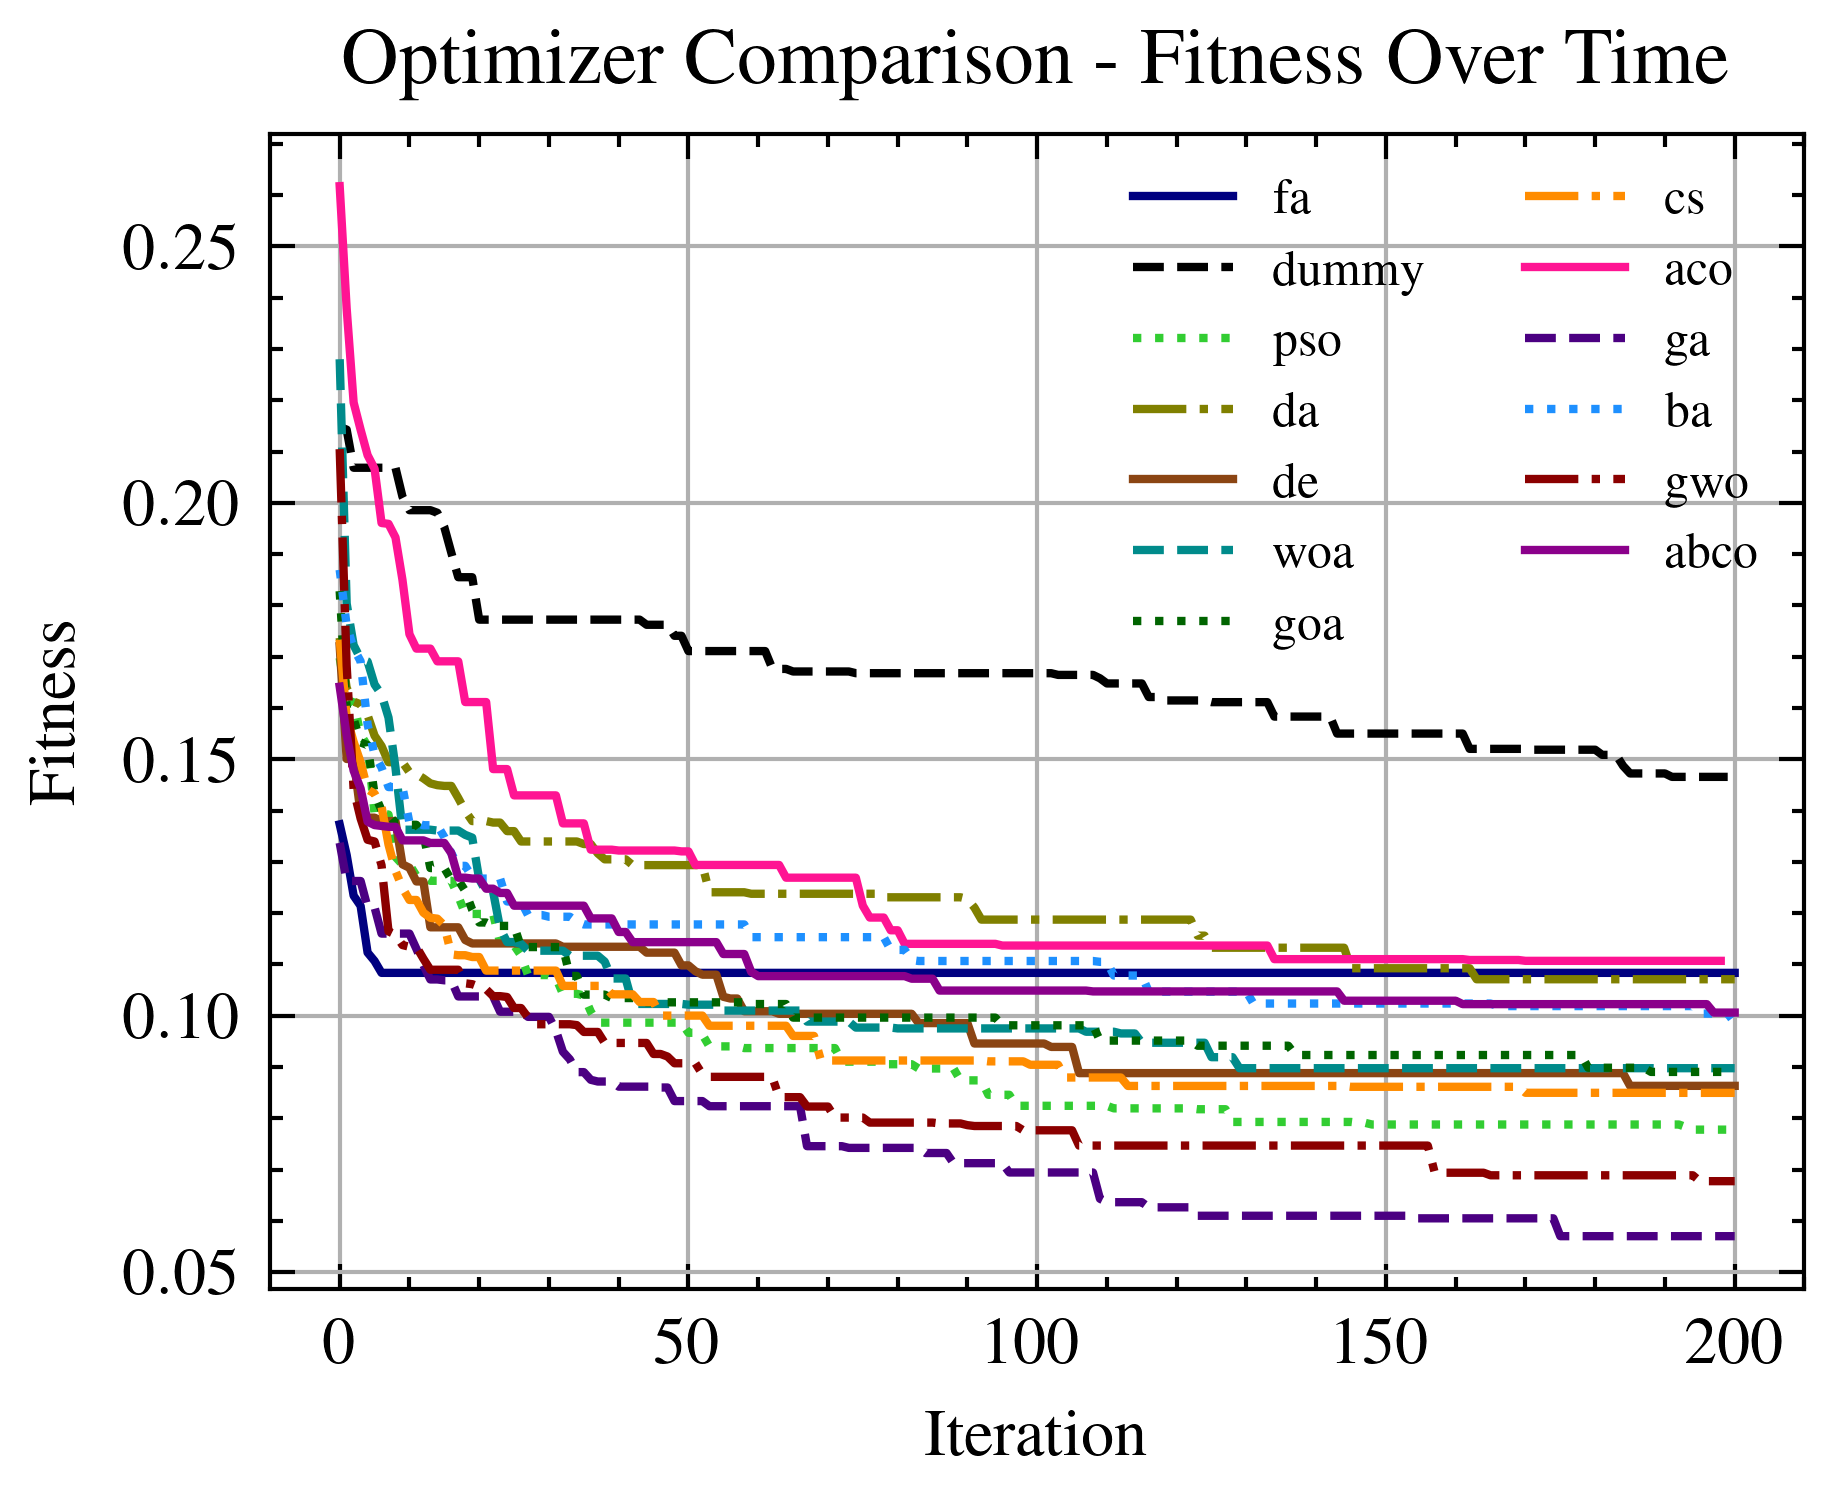
\includegraphics[width=\textwidth]{imagenes/fitness_charts/img/binary/sonar/optimizers_fitness_svc.png}
        \caption{sonar}
        \label{fig:convergencia_sonar_svc}
    \end{subfigure}
    \caption{Convergencia con SVC parte 1 - binario}
    \label{fig:convergencia_svc_1}
\end{figure}

\begin{figure}[htb]
    \centering
    \begin{subfigure}[b]{0.45\textwidth}
        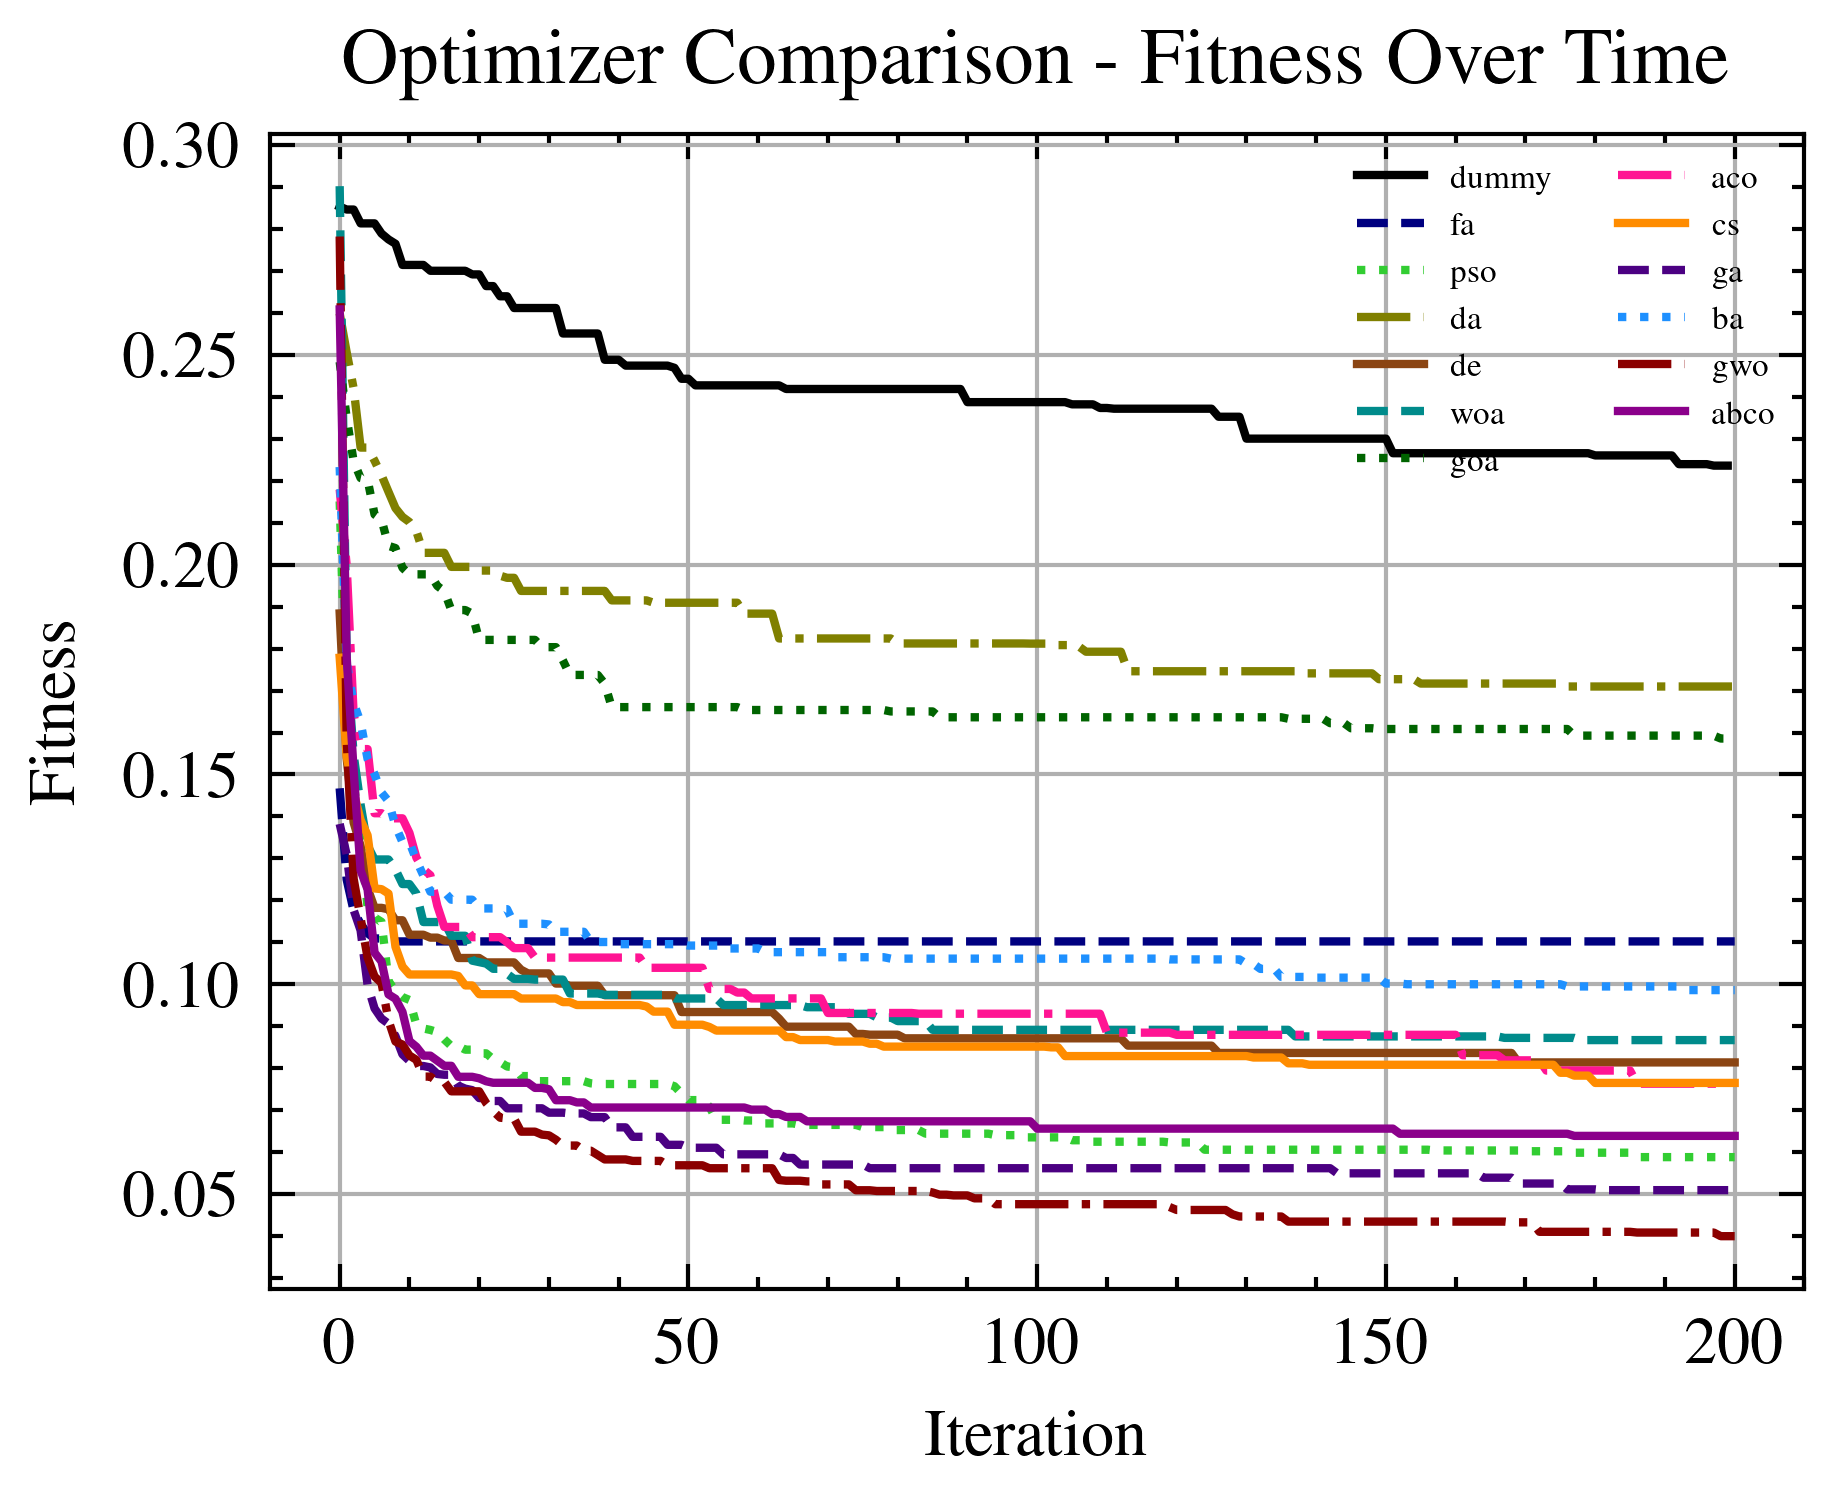
\includegraphics[width=\textwidth]{imagenes/fitness_charts/img/binary/spambase-460/optimizers_fitness_svc.png}
        \caption{spambase-460}
        \label{fig:convergencia_spambase-460_svc}
    \end{subfigure}
    \begin{subfigure}[b]{0.45\textwidth}
        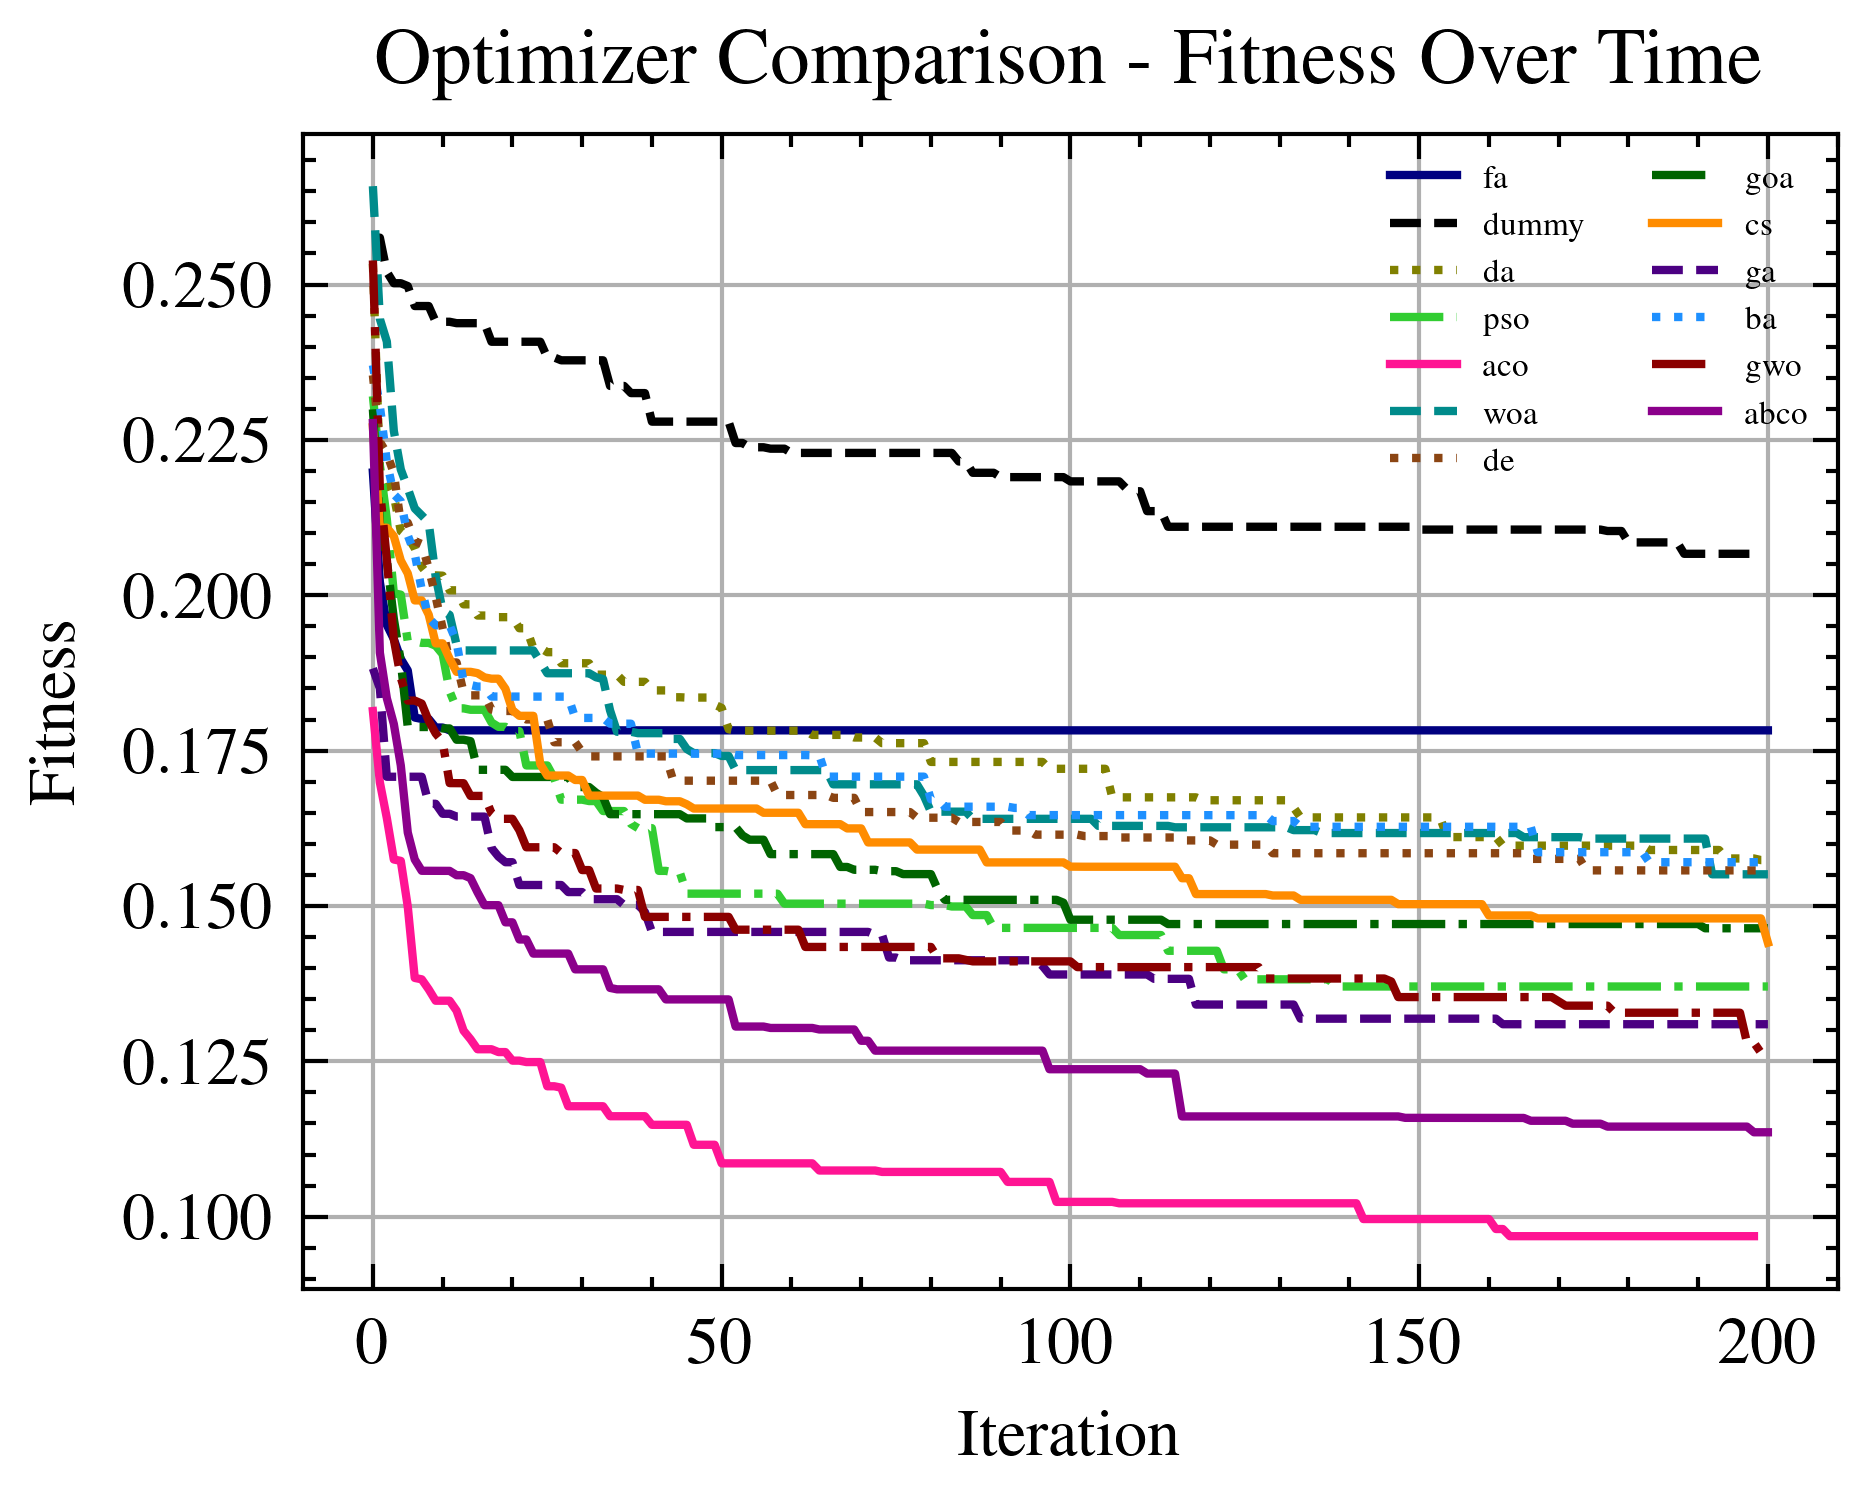
\includegraphics[width=\textwidth]{imagenes/fitness_charts/img/binary/spectf-heart/optimizers_fitness_svc.png}
        \caption{spectf-heart}
        \label{fig:convergencia_spectf-heart_svc}
    \end{subfigure}

    \begin{subfigure}[b]{0.45\textwidth}
        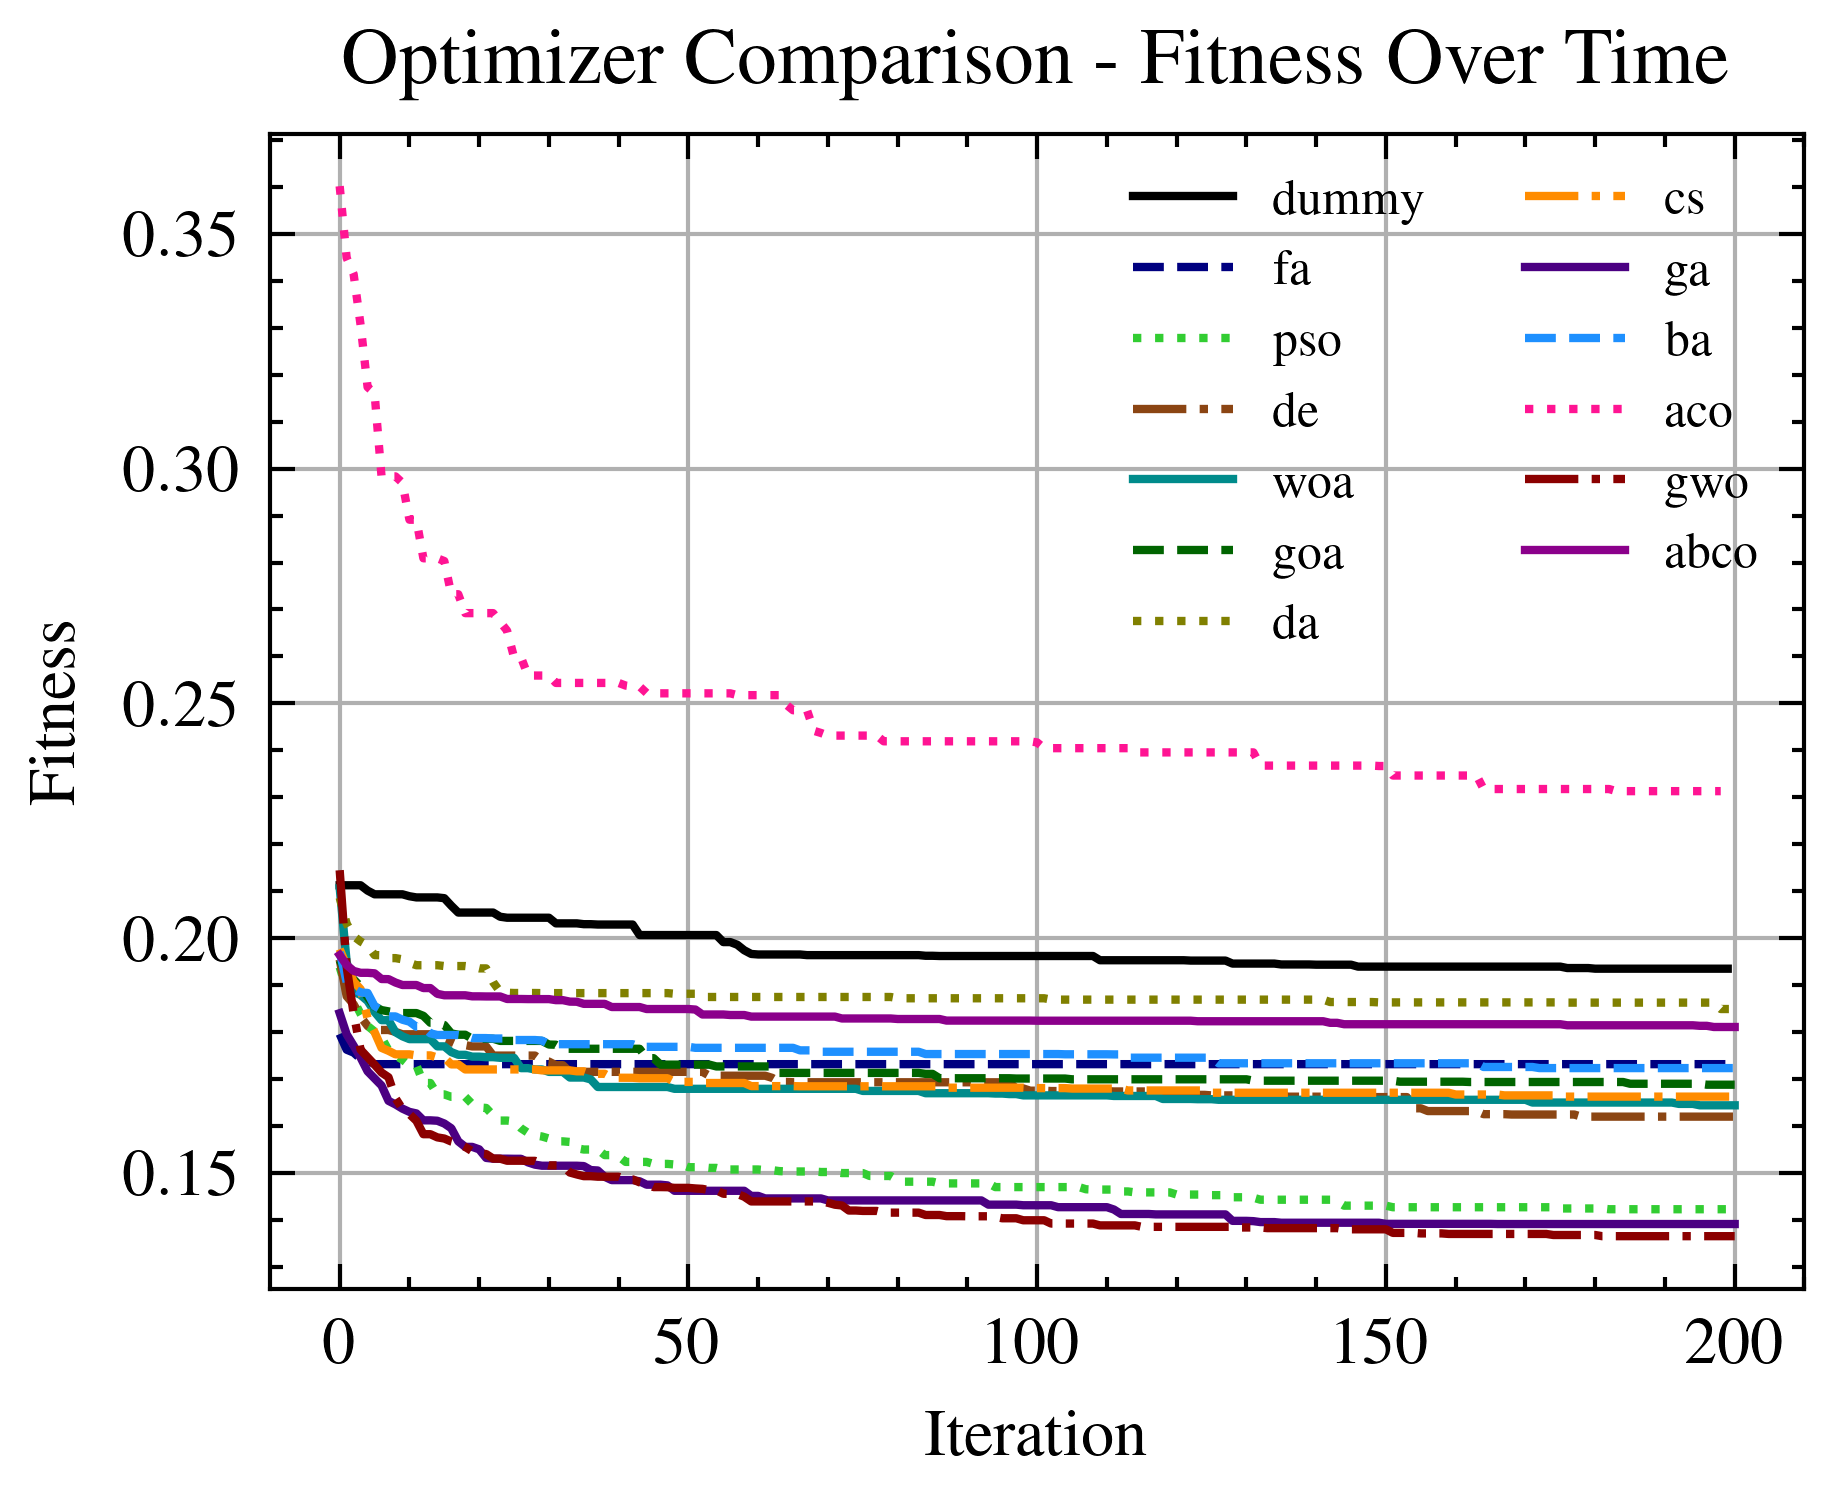
\includegraphics[width=\textwidth]{imagenes/fitness_charts/img/binary/waveform5000/optimizers_fitness_svc.png}
        \caption{waveform5000}
        \label{fig:convergencia_waveform5000_svc}
    \end{subfigure}
    \begin{subfigure}[b]{0.45\textwidth}
        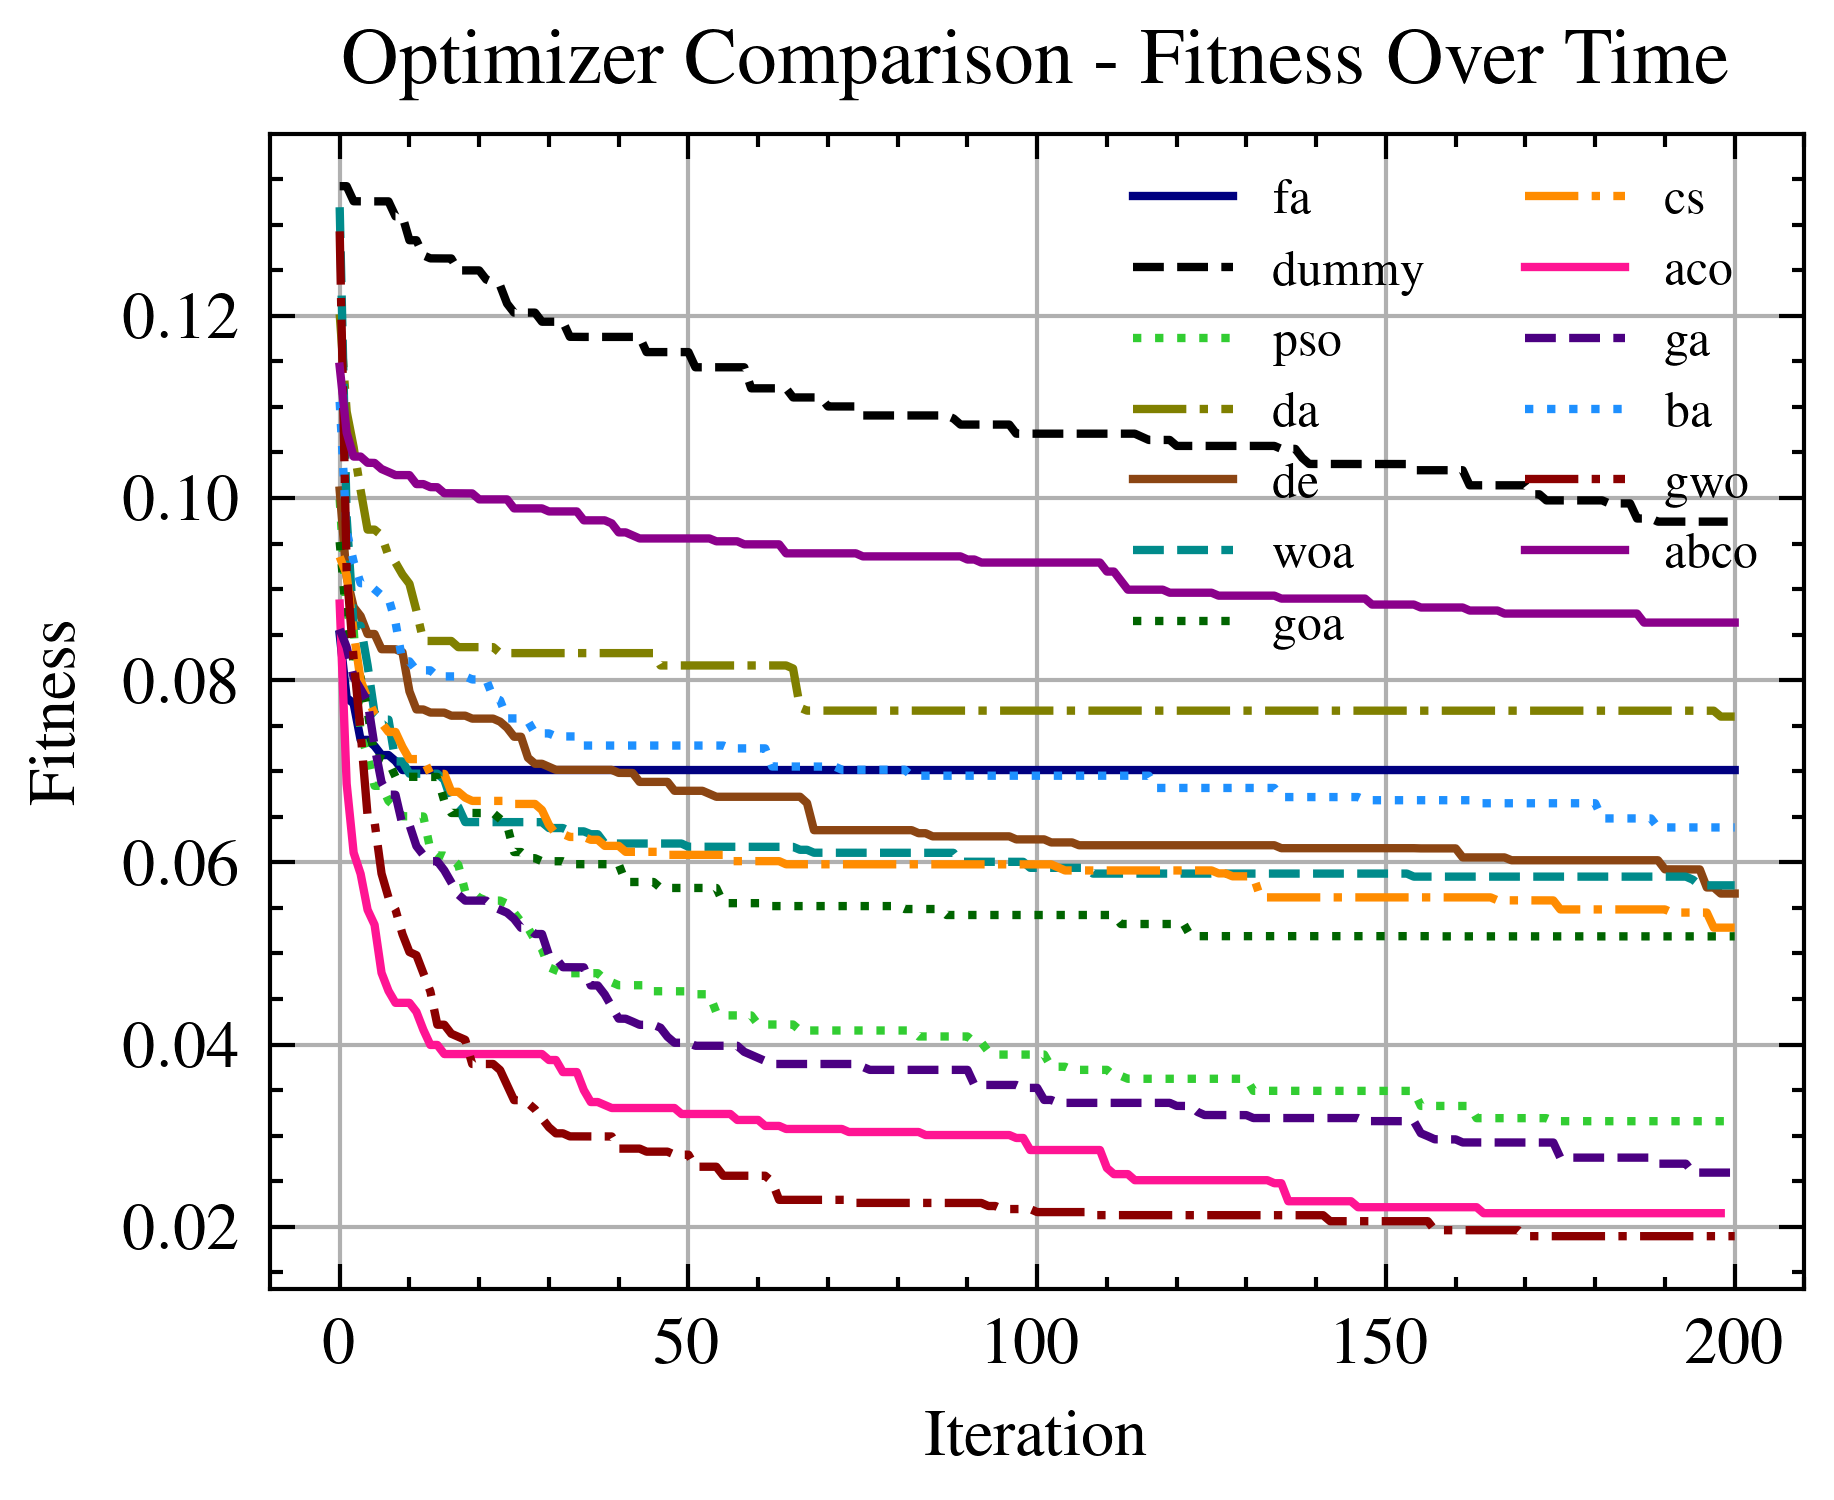
\includegraphics[width=\textwidth]{imagenes/fitness_charts/img/binary/wdbc/optimizers_fitness_svc.png}
        \caption{wdbc}
        \label{fig:convergencia_wdbc_svc}
    \end{subfigure}

    \begin{subfigure}[b]{0.45\textwidth}
        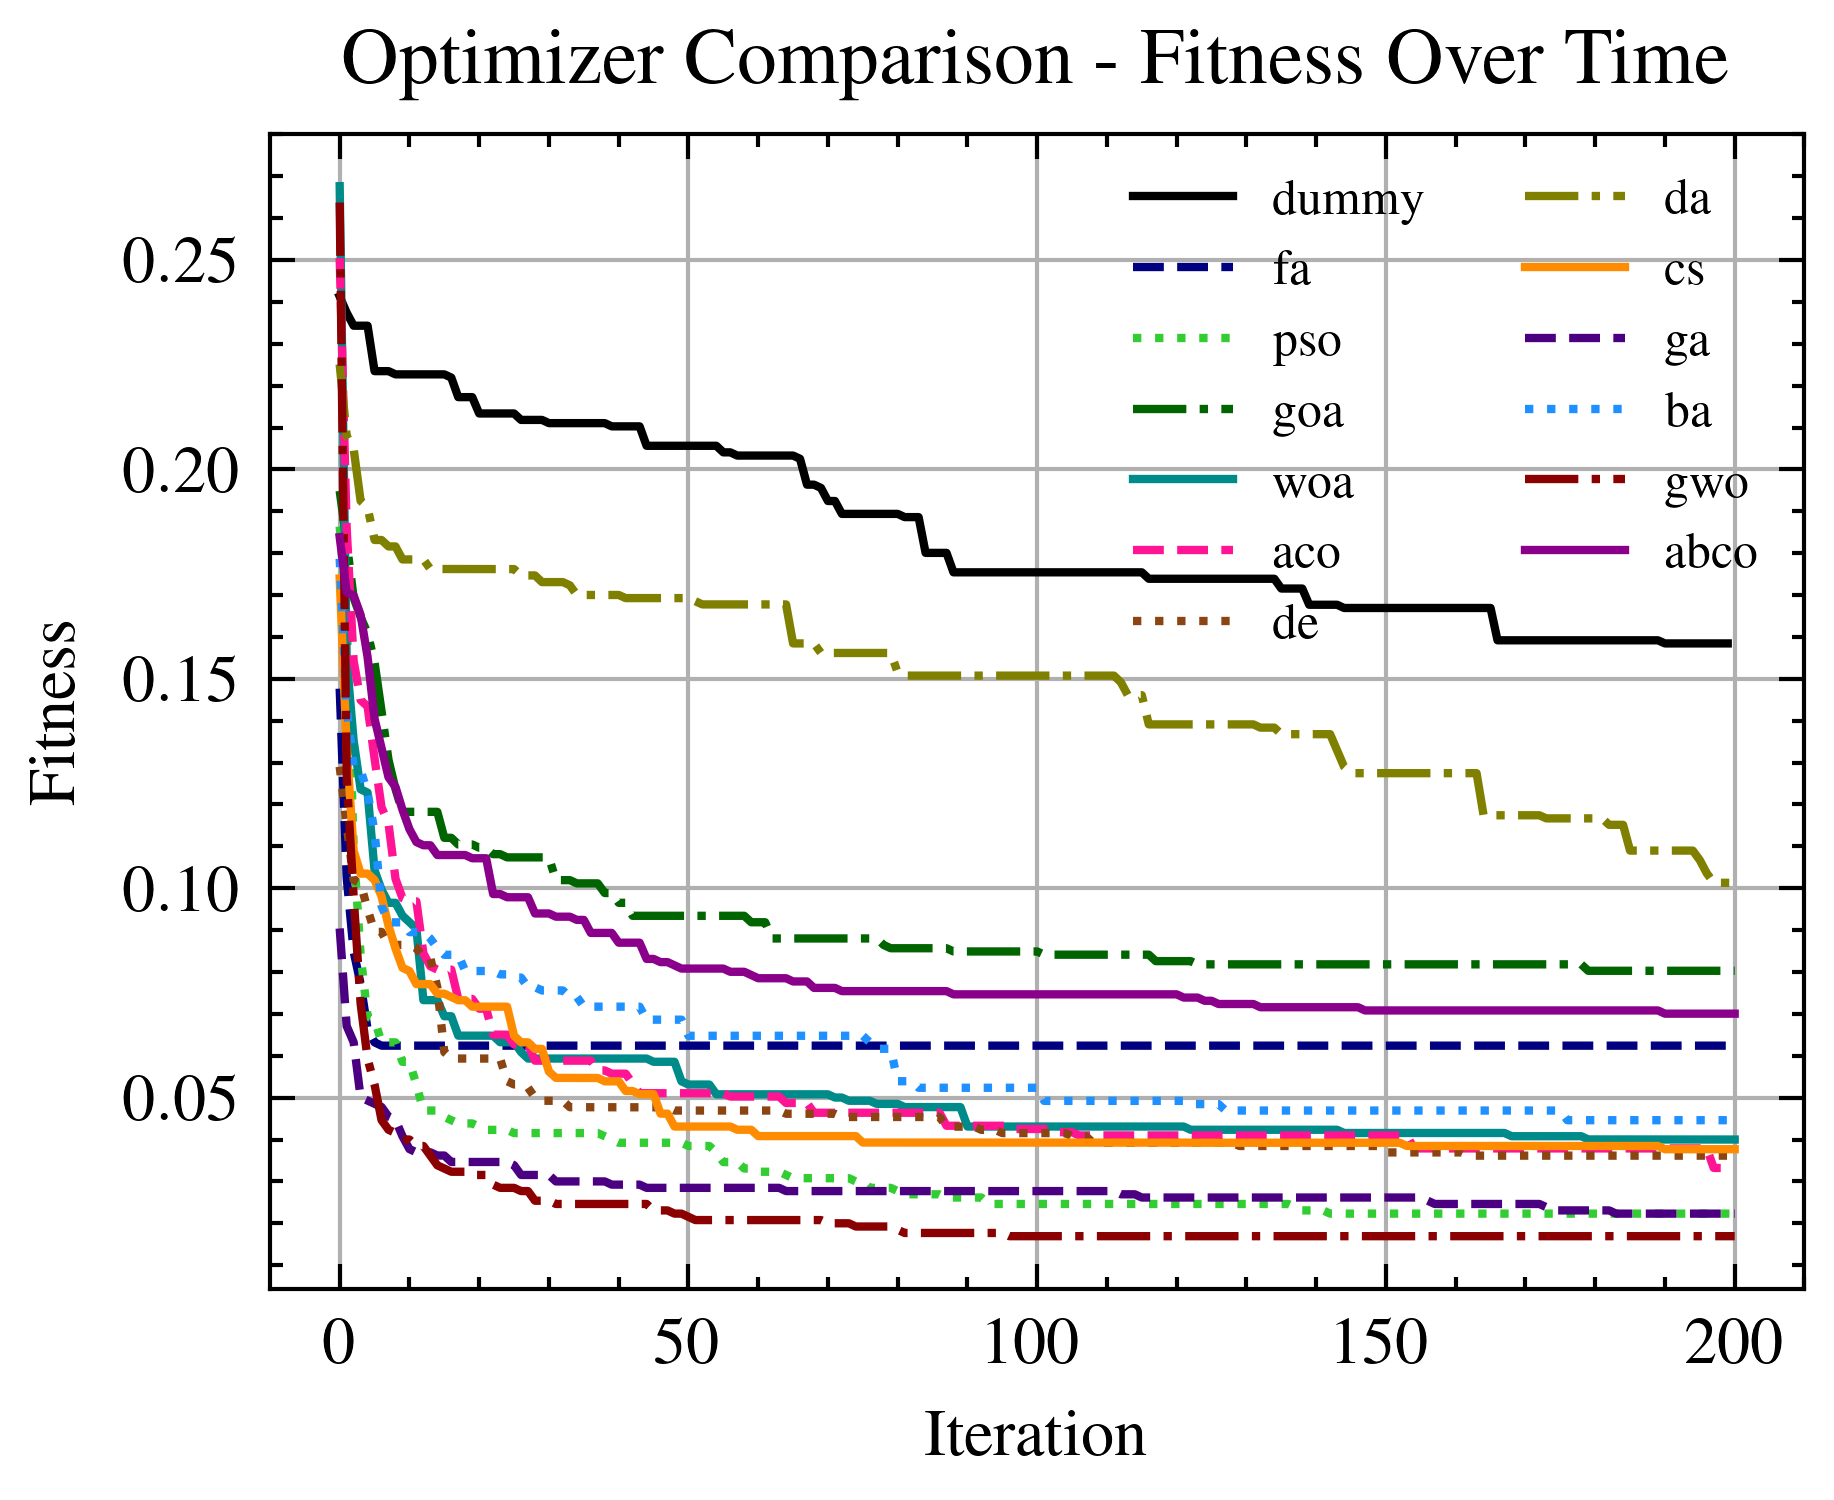
\includegraphics[width=\textwidth]{imagenes/fitness_charts/img/binary/wine/optimizers_fitness_svc.png}
        \caption{wine}
        \label{fig:convergencia_wine_svc}
    \end{subfigure}
    \begin{subfigure}[b]{0.45\textwidth}
        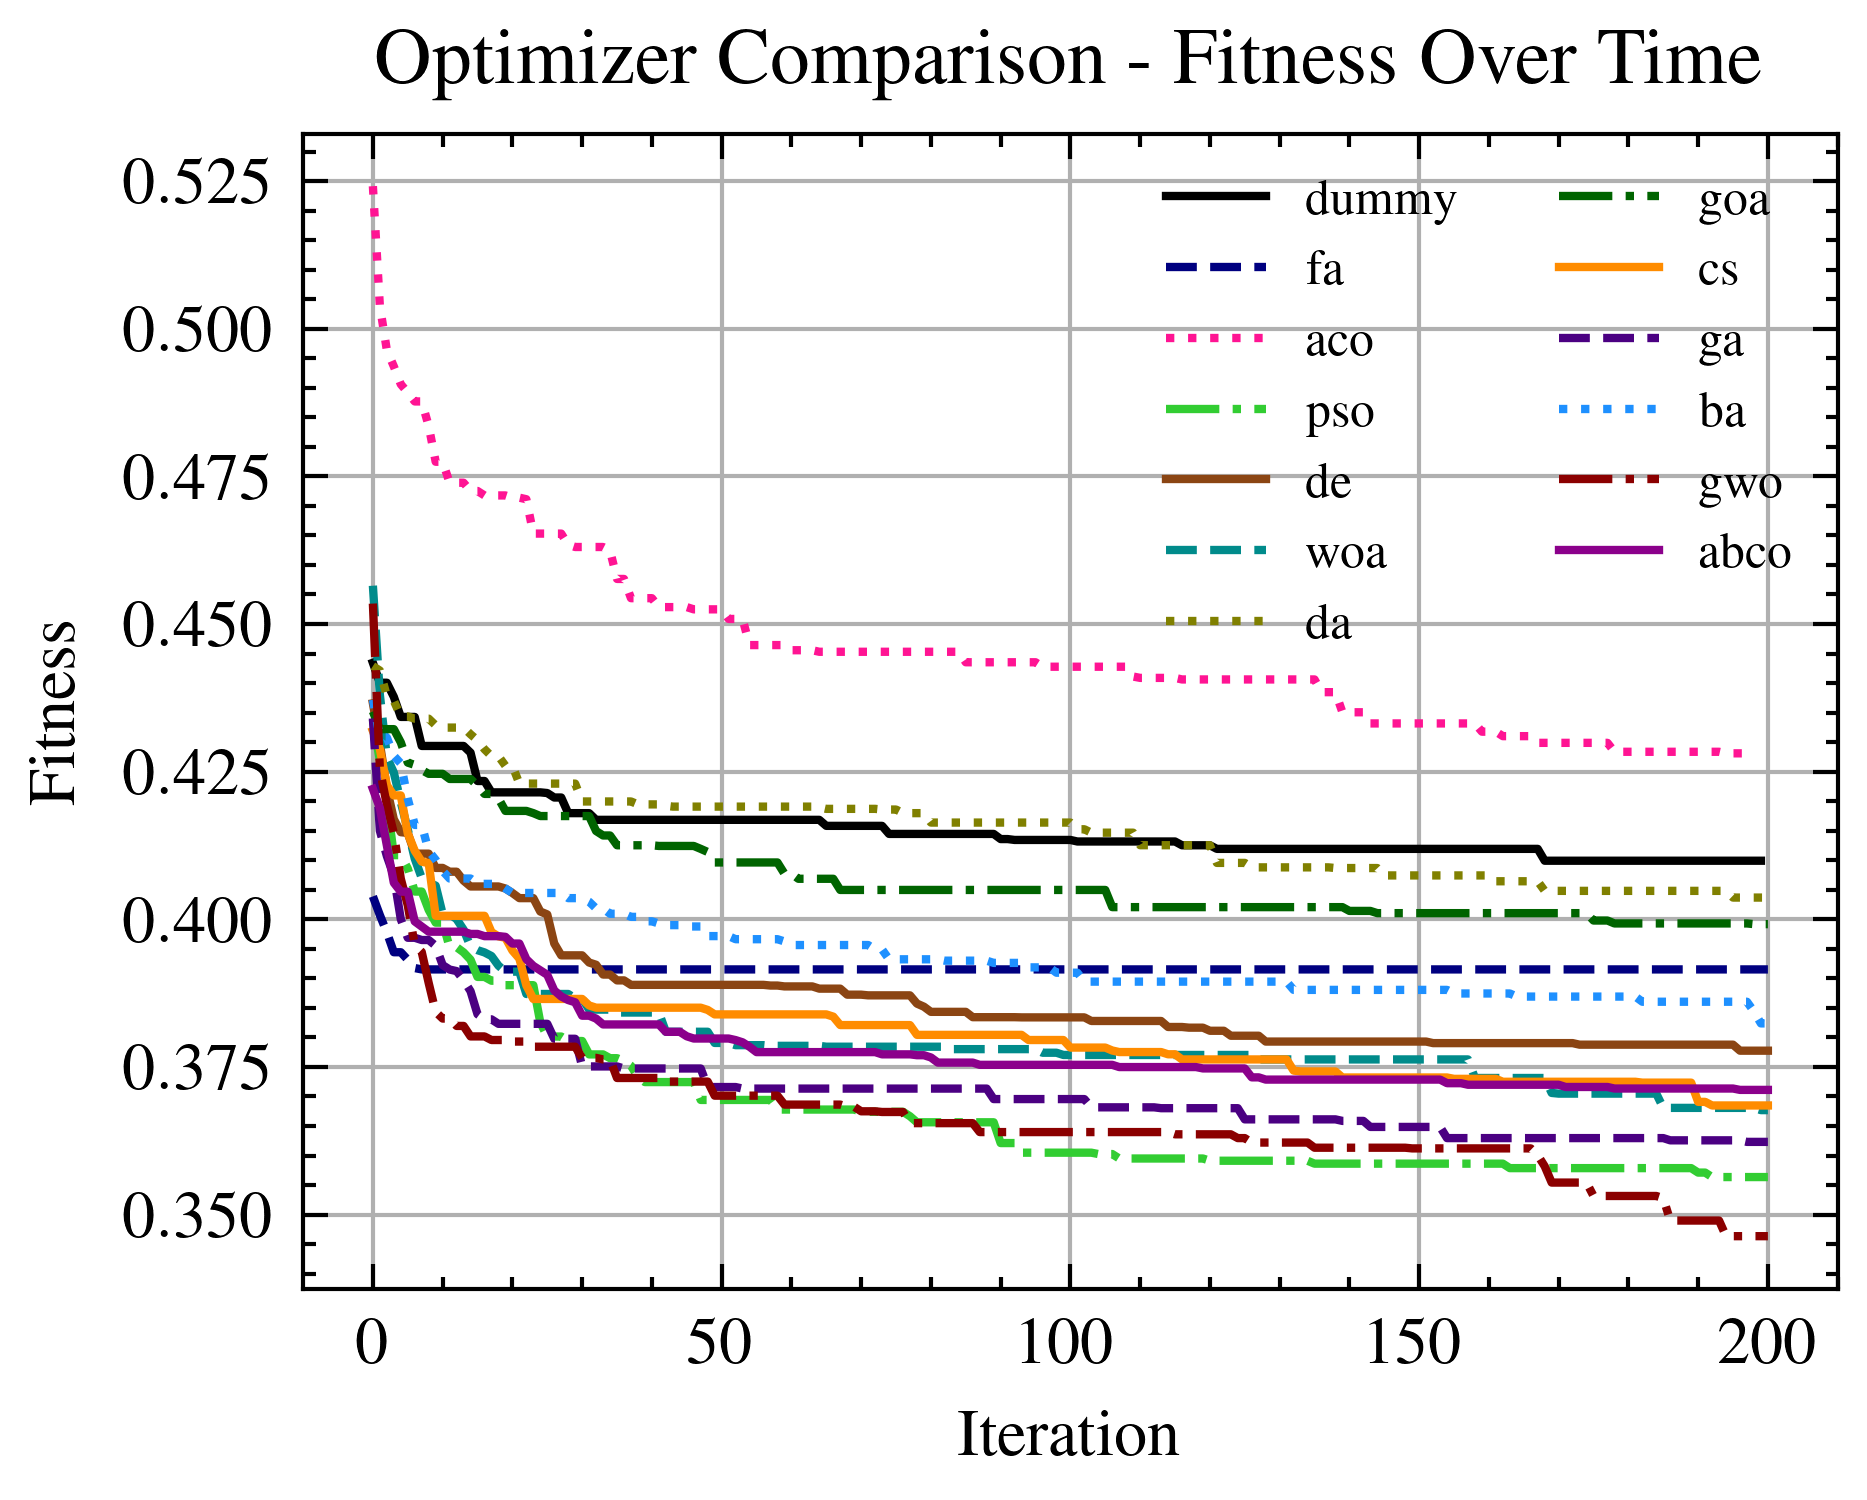
\includegraphics[width=\textwidth]{imagenes/fitness_charts/img/binary/yeast/optimizers_fitness_svc.png}
        \caption{yeast}
        \label{fig:convergencia_yeast_svc}
    \end{subfigure}

    \begin{subfigure}[b]{0.45\textwidth}
        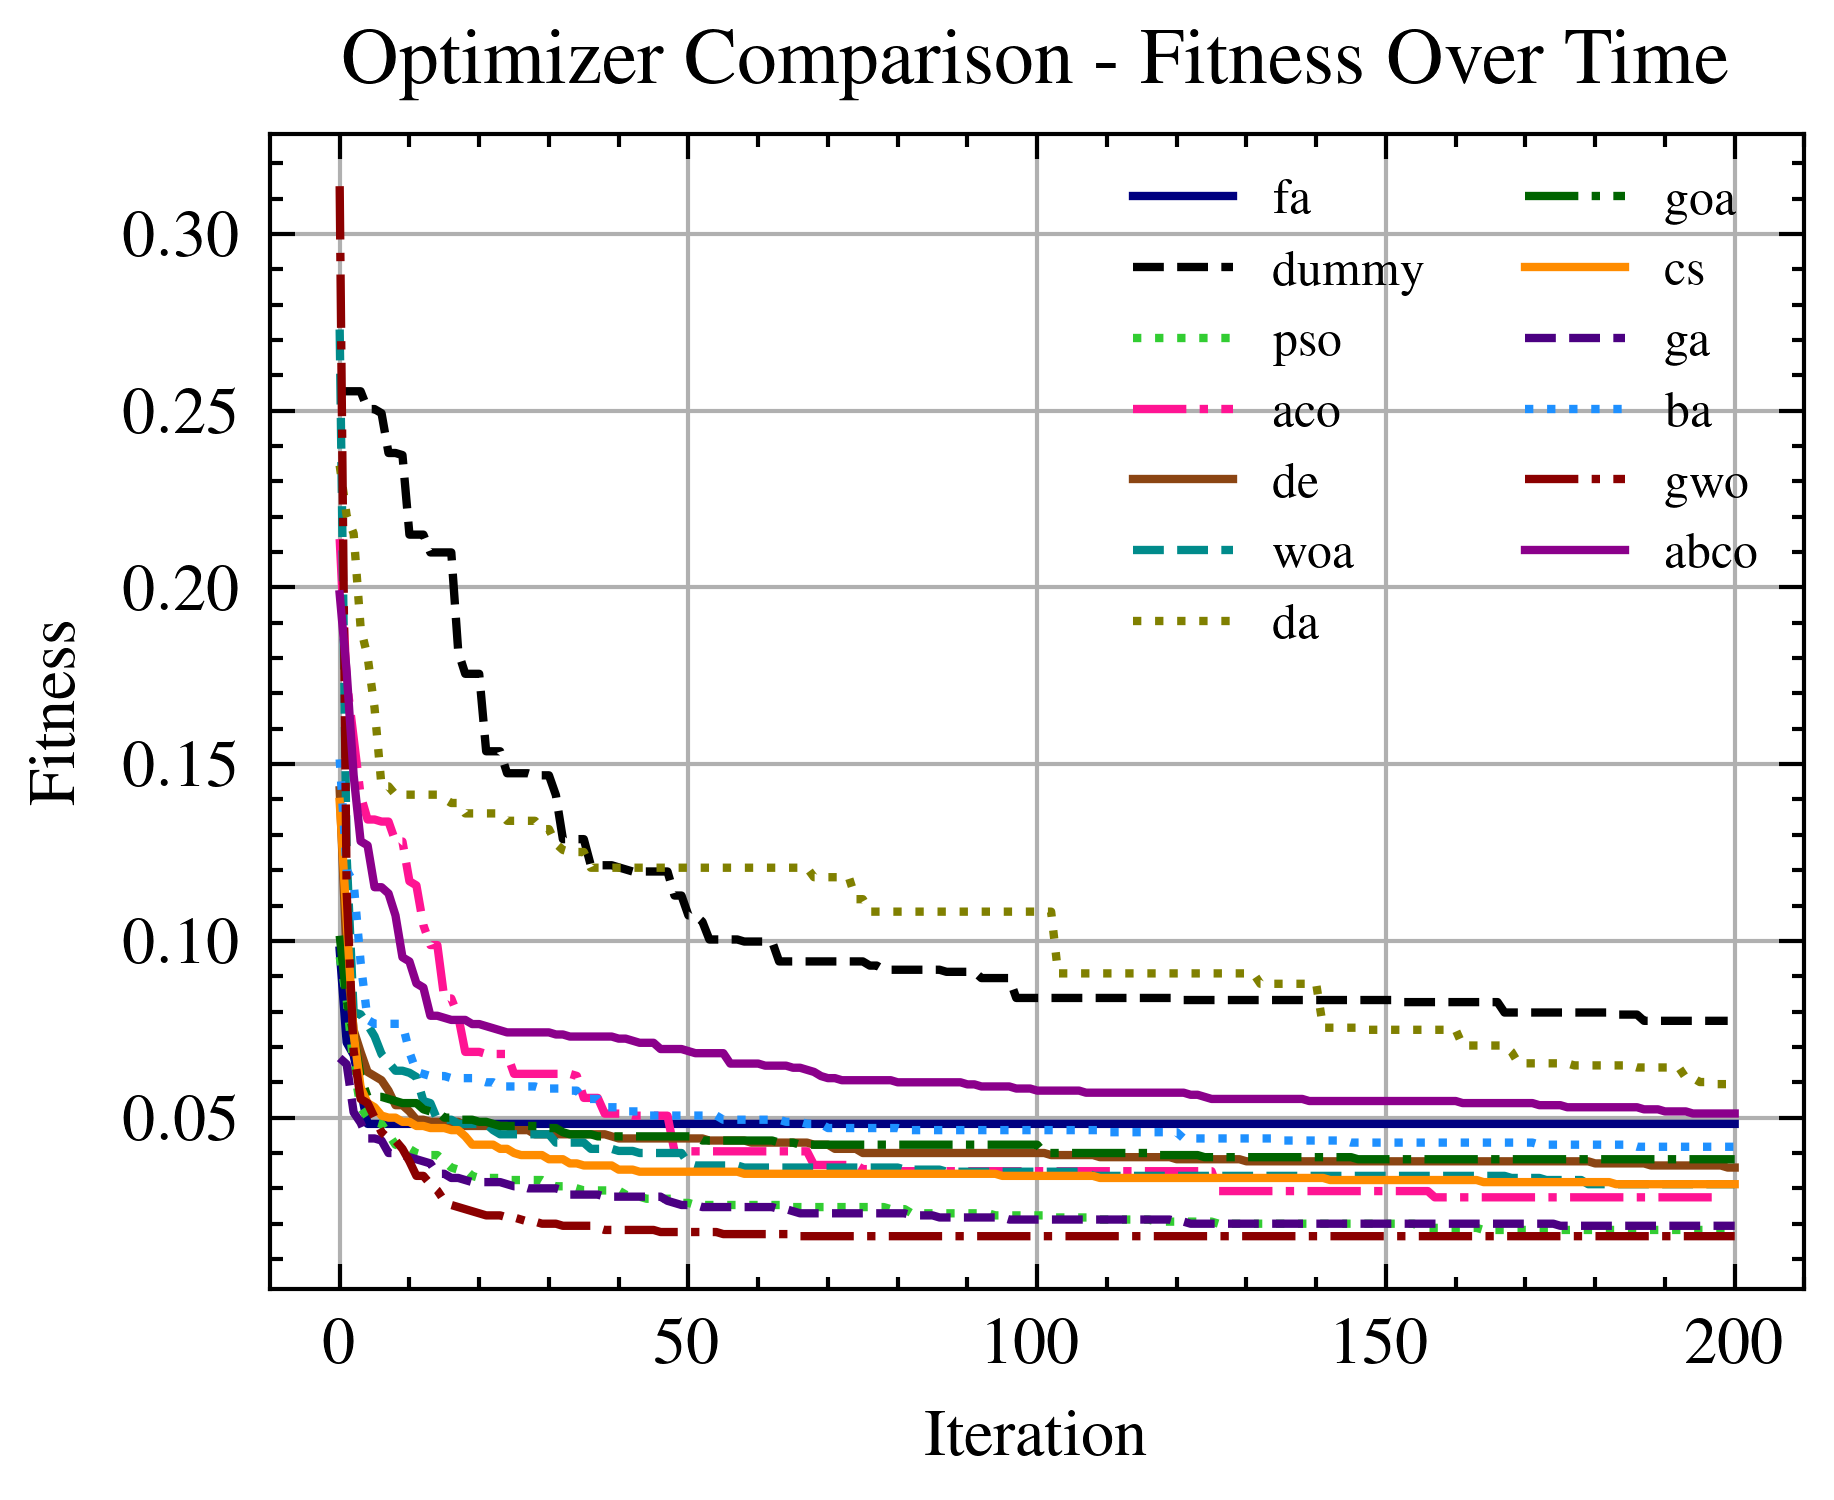
\includegraphics[width=\textwidth]{imagenes/fitness_charts/img/binary/zoo/optimizers_fitness_svc.png}
        \caption{zoo}
        \label{fig:convergencia_zoo_svc}
    \end{subfigure}
    \caption{Convergencia con SVC parte 2 - binario}
    \label{fig:convergencia_svc_2}
\end{figure}

\begin{sidewaystable}[htb]
    \begin{adjustbox}{width=\linewidth}
        \begin{tabular}{llllllllllllllll}
            \toprule
            optimizer & breast-cancer     & dermatology       & diabetes          & ecoli             & ionosphere        & iris              & parkinsons        & sonar             & spambase-460      & spectf-heart      & waveform5000      & wdbc              & wine              & yeast             & zoo    \tabularnewline
            \midrule
            abco      & 3.08E-01          & 1.76E-01          & 3.13E-01          & 2.99E-01          & 2.12E-01          & 1.00E-01          & 2.87E-01          & 4.53E-01          & 3.19E-01          & 2.80E-01          & 2.37E-01          & 1.60E-01          & 3.23E-01          & 5.26E-01          & 3.21E-01\tabularnewline
            aco       & \textbf{1.94E-01} & 2.04E-01          & 2.70E-01          & 3.53E-01          & 1.71E-01          & 1.15E-01          & 2.07E-01          & \textbf{3.33E-01} & 1.74E-01          & \textbf{2.27E-01} & 2.48E-01          & 8.78E-02          & 2.20E-01          & 4.91E-01          & 5.69E-01\tabularnewline
            ba        & 3.46E-01          & 1.62E-01          & 2.76E-01          & 2.68E-01          & 1.64E-01          & 1.45E-01          & 2.24E-01          & 4.47E-01          & 2.58E-01          & 3.13E-01          & 2.04E-01          & 1.35E-01          & 2.70E-01          & 5.09E-01          & 3.84E-01\tabularnewline
            cs        & 3.63E-01          & \textbf{9.01E-02} & 2.67E-01          & \textbf{2.31E-01} & \textbf{1.34E-01} & 1.15E-01          & \textbf{2.01E-01} & 4.26E-01          & 2.08E-01          & 2.91E-01          & 1.92E-01          & 1.44E-01          & 2.96E-01          & 5.00E-01          & 3.01E-01\tabularnewline
            da        & 2.17E-01          & 1.84E-01          & 2.72E-01          & 3.01E-01          & 1.87E-01          & 1.45E-01          & 2.36E-01          & 4.44E-01          & 2.74E-01          & 2.90E-01          & 2.02E-01          & 1.32E-01          & 3.77E-01          & 5.12E-01          & 3.36E-01\tabularnewline
            de        & 3.47E-01          & 1.91E-01          & 3.48E-01          & 2.82E-01          & 1.40E-01          & \textbf{7.00E-02} & 2.48E-01          & 3.63E-01          & 2.67E-01          & 2.74E-01          & 1.92E-01          & 1.31E-01          & \textbf{2.05E-01} & 5.22E-01          & 3.24E-01\tabularnewline
            dummy     & 2.92E-01          & 2.70E-01          & 3.46E-01          & 3.49E-01          & 1.74E-01          & 2.40E-01          & 2.29E-01          & 3.88E-01          & 3.82E-01          & 3.93E-01          & 2.35E-01          & 1.52E-01          & 3.38E-01          & 5.75E-01          & 4.86E-01\tabularnewline
            fa        & 2.58E-01          & 1.21E-01          & 2.88E-01          & 3.23E-01          & 1.57E-01          & 1.20E-01          & 3.10E-01          & 3.86E-01          & 2.14E-01          & 2.84E-01          & 2.04E-01          & 1.31E-01          & 4.10E-01          & 4.98E-01          & \textbf{2.46E-01}\tabularnewline
            ga        & 3.02E-01          & 1.45E-01          & 2.59E-01          & 3.45E-01          & 1.36E-01          & 1.30E-01          & 2.21E-01          & 4.26E-01          & 1.81E-01          & 2.85E-01          & \textbf{1.80E-01} & 1.11E-01          & 3.04E-01          & 4.99E-01          & 3.07E-01\tabularnewline
            goa       & 2.98E-01          & 2.19E-01          & 3.26E-01          & 3.01E-01          & 1.61E-01          & 3.03E-01          & 2.26E-01          & 3.99E-01          & 3.69E-01          & 2.41E-01          & 2.00E-01          & 8.80E-02          & 4.06E-01          & 5.41E-01          & 4.34E-01\tabularnewline
            gwo       & 3.11E-01          & 1.73E-01          & 2.61E-01          & 2.79E-01          & 1.46E-01          & 1.15E-01          & 2.44E-01          & 3.34E-01          & \textbf{1.72E-01} & 2.77E-01          & 1.92E-01          & \textbf{5.51E-02} & 2.64E-01          & 4.81E-01          & 3.04E-01\tabularnewline
            pso       & 2.82E-01          & 1.30E-01          & 2.60E-01          & 2.92E-01          & 1.38E-01          & 1.30E-01          & 2.54E-01          & 3.89E-01          & 2.40E-01          & 2.78E-01          & 1.87E-01          & 1.15E-01          & 2.14E-01          & \textbf{4.59E-01} & 3.24E-01\tabularnewline
            woa       & 2.64E-01          & 1.61E-01          & \textbf{2.27E-01} & 2.61E-01          & 1.68E-01          & 1.15E-01          & 2.66E-01          & 3.68E-01          & 1.91E-01          & 3.54E-01          & 1.84E-01          & 1.11E-01          & 3.33E-01          & 5.22E-01          & 3.55E-01\tabularnewline
            \bottomrule
        \end{tabular}
    \end{adjustbox}
    \caption{Fitness medio con clasificador SVC - binario}
    \label{tab:fitness_svc}
\end{sidewaystable}

\begin{sidewaystable}[htb]
    \begin{adjustbox}{width=\linewidth}
        \begin{tabular}{llllllllllllllll}
            \toprule
            optimizer & breast-cancer     & dermatology       & diabetes          & ecoli             & ionosphere        & iris              & parkinsons        & sonar             & spambase-460      & spectf-heart      & waveform5000      & wdbc              & wine              & yeast             & zoo\tabularnewline
            \midrule
            abco      & 3.64E-01          & 1.76E-01          & 3.39E-01          & 3.15E-01          & 3.11E-01          & 1.00E-01          & 2.10E-01          & 4.22E-01          & 2.88E-01          & 3.44E-01          & 2.72E-01          & 1.77E-01          & 2.66E-01          & 5.07E-01          & 3.94E-01\tabularnewline
            aco       & \textbf{2.35E-01} & 2.88E-01          & 3.15E-01          & 2.80E-01          & 2.34E-01          & 8.50E-02          & 2.30E-01          & 3.75E-01          & 2.60E-01          & 3.55E-01          & 2.85E-01          & 1.22E-01          & 2.07E-01          & 5.12E-01          & 3.90E-01\tabularnewline
            ba        & 2.96E-01          & 1.59E-01          & 3.29E-01          & 3.31E-01          & 2.49E-01          & \textbf{2.50E-02} & 1.98E-01          & 4.05E-01          & 2.38E-01          & 3.20E-01          & 2.44E-01          & 1.15E-01          & 1.85E-01          & 5.05E-01          & 4.21E-01\tabularnewline
            cs        & 3.33E-01          & 1.90E-01          & 3.16E-01          & \textbf{1.95E-01} & 3.08E-01          & 1.00E-01          & 2.08E-01          & 4.28E-01          & \textbf{1.66E-01} & 2.82E-01          & 2.42E-01          & 1.15E-01          & 2.41E-01          & 5.25E-01          & 3.57E-01\tabularnewline
            da        & 3.56E-01          & 2.00E-01          & 2.83E-01          & 2.51E-01          & 2.71E-01          & 5.50E-02          & \textbf{1.76E-01} & 4.62E-01          & 2.97E-01          & 3.29E-01          & 2.64E-01          & 1.49E-01          & 1.88E-01          & 5.46E-01          & 4.20E-01\tabularnewline
            de        & 3.54E-01          & 1.46E-01          & 3.23E-01          & 2.81E-01          & 2.51E-01          & 1.00E-01          & 3.26E-01          & \textbf{3.70E-01} & 1.94E-01          & \textbf{2.79E-01} & 2.34E-01          & 1.63E-01          & 1.79E-01          & 5.04E-01          & 3.96E-01\tabularnewline
            dummy     & 4.33E-01          & 2.34E-01          & 3.56E-01          & 3.03E-01          & 3.10E-01          & 1.45E-01          & 2.45E-01          & 4.76E-01          & 3.25E-01          & 3.04E-01          & 2.81E-01          & 1.63E-01          & 3.33E-01          & 5.13E-01          & 4.83E-01\tabularnewline
            fa        & 4.21E-01          & 1.46E-01          & 2.89E-01          & 2.68E-01          & \textbf{2.02E-01} & 2.75E-02          & 2.36E-01          & 4.53E-01          & 2.42E-01          & 3.08E-01          & 2.40E-01          & 1.30E-01          & 1.61E-01          & 5.13E-01          & 4.81E-01\tabularnewline
            ga        & 2.64E-01          & 1.25E-01          & 3.31E-01          & 2.94E-01          & 2.24E-01          & 8.50E-02          & 2.49E-01          & 3.82E-01          & 2.03E-01          & 3.03E-01          & 2.09E-01          & \textbf{9.70E-02} & 2.43E-01          & 5.13E-01          & 4.52E-01\tabularnewline
            goa       & 3.57E-01          & 2.16E-01          & 3.19E-01          & 3.14E-01          & 2.39E-01          & 1.32E-01          & 2.03E-01          & 3.90E-01          & 2.96E-01          & 3.41E-01          & 2.29E-01          & 1.18E-01          & 2.40E-01          & 5.61E-01          & 3.79E-01\tabularnewline
            gwo       & 2.63E-01          & \textbf{1.01E-01} & \textbf{2.78E-01} & 2.29E-01          & 2.27E-01          & 8.50E-02          & 2.14E-01          & 4.41E-01          & 1.89E-01          & 2.89E-01          & \textbf{2.06E-01} & 1.05E-01          & 1.05E-01          & 4.92E-01          & 4.31E-01\tabularnewline
            pso       & 3.41E-01          & 1.21E-01          & 2.95E-01          & 2.16E-01          & 2.60E-01          & 8.50E-02          & 2.33E-01          & 3.78E-01          & 2.21E-01          & 2.99E-01          & 2.11E-01          & 1.12E-01          & 2.07E-01          & \textbf{4.56E-01} & 3.60E-01\tabularnewline
            woa       & 3.23E-01          & 1.58E-01          & 3.34E-01          & 2.63E-01          & 2.17E-01          & 1.00E-01          & 2.59E-01          & 4.05E-01          & 2.02E-01          & 3.09E-01          & 2.48E-01          & 1.16E-01          & \textbf{1.04E-01} & 5.26E-01          & \textbf{2.13E-01}\tabularnewline
            \bottomrule
        \end{tabular}
    \end{adjustbox}
    \caption{Fitness medio con clasificador kNN}
    \label{tab:fitness_knn}
\end{sidewaystable}

\begin{sidewaystable}[htb]
    \begin{adjustbox}{width=\linewidth}
        \begin{tabular}{lllllllllllllllllllllllllll}
            \toprule
            {}            & abco\_knn & abco\_svc & aco\_knn & aco\_svc   & ba\_knn    & ba\_svc & cs\_knn    & cs\_svc    & da\_knn    & da\_svc & de\_knn & de\_svc & dummy\_knn & dummy\_svc & fa\_knn & fa\_svc & ga\_knn & ga\_svc    & goa\_knn & goa\_svc & gwo\_knn & gwo\_svc       & pso\_knn   & pso\_svc & woa\_knn   & woa\_svc   \\
            \midrule
            breast-cancer & 24        & 13        & 3        & \textbf{1} & 10         & 18      & 16         & 23         & 21         & 2       & 20      & 19      & 26         & 9          & 25      & 4       & 6.5     & 12         & 22       & 11       & 5        & 14             & 17         & 8        & 15         & 6.5        \\
            dermatology   & 15.5      & 15.5      & 26       & 21         & 11         & 13      & 18         & \textbf{1} & 20         & 17      & 8.5     & 19      & 24         & 25         & 8.5     & 3.5     & 5       & 7          & 22       & 23       & 2        & 14             & 3.5        & 6        & 10         & 12         \\
            diabetes      & 23        & 14        & 15       & 6          & 20         & 8       & 16         & 5          & 10         & 7       & 18      & 25      & 26         & 24         & 12      & 11      & 21      & 2          & 17       & 19       & 9        & 4              & 13         & 3        & 22         & \textbf{1} \\
            ecoli         & 21        & 16        & 11       & 26         & 23         & 8.5     & \textbf{1} & 4          & 5          & 17.5    & 12      & 13      & 19         & 25         & 8.5     & 22      & 15      & 24         & 20       & 17.5     & 3        & 10             & 2          & 14       & 7          & 6          \\
            ionosphere    & 26        & 14        & 18       & 10         & 20         & 8       & 24         & \textbf{1} & 23         & 12      & 21      & 4       & 25         & 11         & 13      & 6       & 16      & 2          & 19       & 7        & 17       & 5              & 22         & 3        & 15         & 9          \\
            iris          & 11        & 11        & 6.5      & 15.5       & \textbf{1} & 23      & 11         & 15.5       & 3          & 23      & 11      & 4       & 23         & 25         & 2       & 18      & 6.5     & 19.5       & 21       & 26       & 6.5      & 15.5           & 6.5        & 19.5     & 11         & 15.5       \\
            parkinsons    & 7         & 24        & 13       & 5          & 2          & 10      & 6          & 3          & \textbf{1} & 15.5    & 26      & 19      & 18         & 12         & 15.5    & 25      & 20      & 9          & 4        & 11       & 8        & 17             & 14         & 21       & 22         & 23         \\
            sonar         & 16        & 23.5      & 6        & \textbf{1} & 14.5       & 22      & 19         & 17.5       & 25         & 21      & 5       & 3       & 26         & 10         & 23.5    & 9       & 8       & 17.5       & 12       & 13       & 20       & 2              & 7          & 11       & 14.5       & 4          \\
            spambase-460  & 20        & 23        & 17       & 3          & 13         & 16      & \textbf{1} & 10         & 22         & 19      & 7       & 18      & 24         & 26         & 15      & 11      & 9       & 4          & 21       & 25       & 5        & 2              & 12         & 14       & 8          & 6          \\
            spectf-heart  & 23        & 7         & 25       & \textbf{1} & 20         & 19      & 8          & 13         & 21         & 12      & 6       & 3       & 16         & 26         & 17      & 9       & 15      & 10         & 22       & 2        & 11       & 4              & 14         & 5        & 18         & 24         \\
            waveform5000  & 24        & 17        & 26       & 21.5       & 20         & 9.5     & 19         & 5          & 23         & 8       & 15      & 5       & 25         & 16         & 18      & 9.5     & 12      & \textbf{1} & 14       & 7        & 11       & 5              & 13         & 3        & 21.5       & 2          \\
            wdbc          & 26        & 23        & 14       & 2          & 10         & 19      & 10         & 20         & 21         & 18      & 24.5    & 16.5    & 24.5       & 22         & 15      & 16.5    & 4       & 6.5        & 13       & 3        & 5        & \textbf{1}     & 8          & 10       & 12         & 6.5        \\
            wine          & 16        & 20        & 8.5      & 11         & 5          & 17      & 13         & 18         & 6          & 24      & 4       & 7       & 21.5       & 23         & 3       & 26      & 14      & 19         & 12       & 25       & 2        & 15             & 8.5        & 10       & \textbf{1} & 21.5       \\
            yeast         & 11        & 21        & 13.5     & 4          & 9.5        & 12      & 20         & 8          & 24         & 13.5    & 9.5     & 18      & 16         & 26         & 16      & 6       & 16      & 7          & 25       & 23       & 5        & 3              & \textbf{1} & 2        & 22         & 19         \\
            zoo           & 16        & 6         & 15       & 26         & 19         & 14      & 11         & 3          & 18         & 9       & 17      & 7.5     & 24         & 25         & 23      & 2       & 22      & 5          & 13       & 21       & 20       & 4              & 12         & 7.5      & \textbf{1} & 10         \\
            \midrule
            Mean          & 18.633    & 16.533    & 14.500   & 10.267     & 13.200     & 14.467  & 12.867     & 9.800      & 16.200     & 14.567  & 13.633  & 12.067  & 22.533     & 20.333     & 14.333  & 11.900  & 12.667  & 9.700      & 17.133   & 15.567   & 8.633    & \textbf{7.700} & 10.233     & 9.133    & 13.333     & 11.067     \\
            \bottomrule
        \end{tabular}
    \end{adjustbox}
    \caption{Ranking de los algoritmos en \textit{fitness} - binario}
    \label{tab:ranking_fitness_bin}
\end{sidewaystable}
\clearpage

\subsection{Clasificación y reducción}
Como se ha mencionado al principio de la anterior sección y como se explica en la fórmula \ref{eq:fitness}, el \textit{fitness} está compuesto por las métricas de \textit{accuracy} en la clasificación y por el ratio de reducción de las características. Con ello se intenta reducir tantas características como sea posible, manteniendo un valor lo más alto posible de precisión.\\[6pt]
Con estos aspectos aclarados, en esta sección se analizarán los algoritmos desde la perspectiva individual de cada una de las métricas que componen la función \textit{fitness}. De esta manera, se proveerá información de cuál o cuáles algoritmos son los mejores para cada una de las métricas.\\[6pt]
Esta visión es interesante ya que, los pesos fijados por el autor para cada métrica son los estándar en la mayoría de artículos, pero es posible que en otros problemas sea necesario ajustarlos a las necesidades del mismo. Por tanto si se conocen las características de los diferentes algoritmos para cada métrica por separado, se obtendrá un conocimiento que proporcionará un uso de los mismos más flexible.

\subsubsection{Clásicos vs Modernos}
Se procede a comparar los algoritmos clásicos frente a los algoritmos modernos en cuanto a su capacidad clasificatoria, es decir, el valor de cada uno de ellos obtenido en \textit{accuracy}.\\[6pt]

En los rankings definidos en la tabla \ref{tab:ranking_acc_bin}, queda claro que \textbf{bCS} usando el algoritmo \textbf{SVC} es capaz de obtener los mejores resultados en cuanto a la precisión en la clasificación. Le siguen algoritmos como \textbf{bDE}, \textbf{bGWO} o \textbf{bFA}.\\[6pt]

Si bien es cierto que la mayoría en el top de mejores algoritmos en \textit{accuracy} son algoritmos modernos, los clásicos no se quedan atrás. En las comparaciones obtienen muy buenos resultados, no siendo los mejores y muy lejos de ser los peores. En los algoritmos modernos hay mayor diversidad en este punto. Hay unos pocos que destacan, pero el resto parece verse superado en muchas ocasiones por los algoritmos clásicos.\\[6pt]

Pese a ello, se puede apreciar en la tabla \ref{tab:p-values_accuracy} como algoritmos como \textbf{bPSO} no obtienen resultados significativos con respecto al resto de sus competidores. Si se comparan los p-valores de los algoritmos modernos con los de los clásicos, se aprecia que, a excepción de algunos algoritmos como \textbf{bDummy} (obviamente) y \textbf{ACO}, no hay diferencia estadísticamente suficientemente significativa como para determinar que un grupo de algoritmos es mejor que otro. De hecho, al corregir estos valores usando un post hoc como \textbf{Holms}, las diferencias son incluso menores.\\[6pt]

\begin{figure}[htb]
    \centering
    \begin{subfigure}[b]{1\textwidth}
        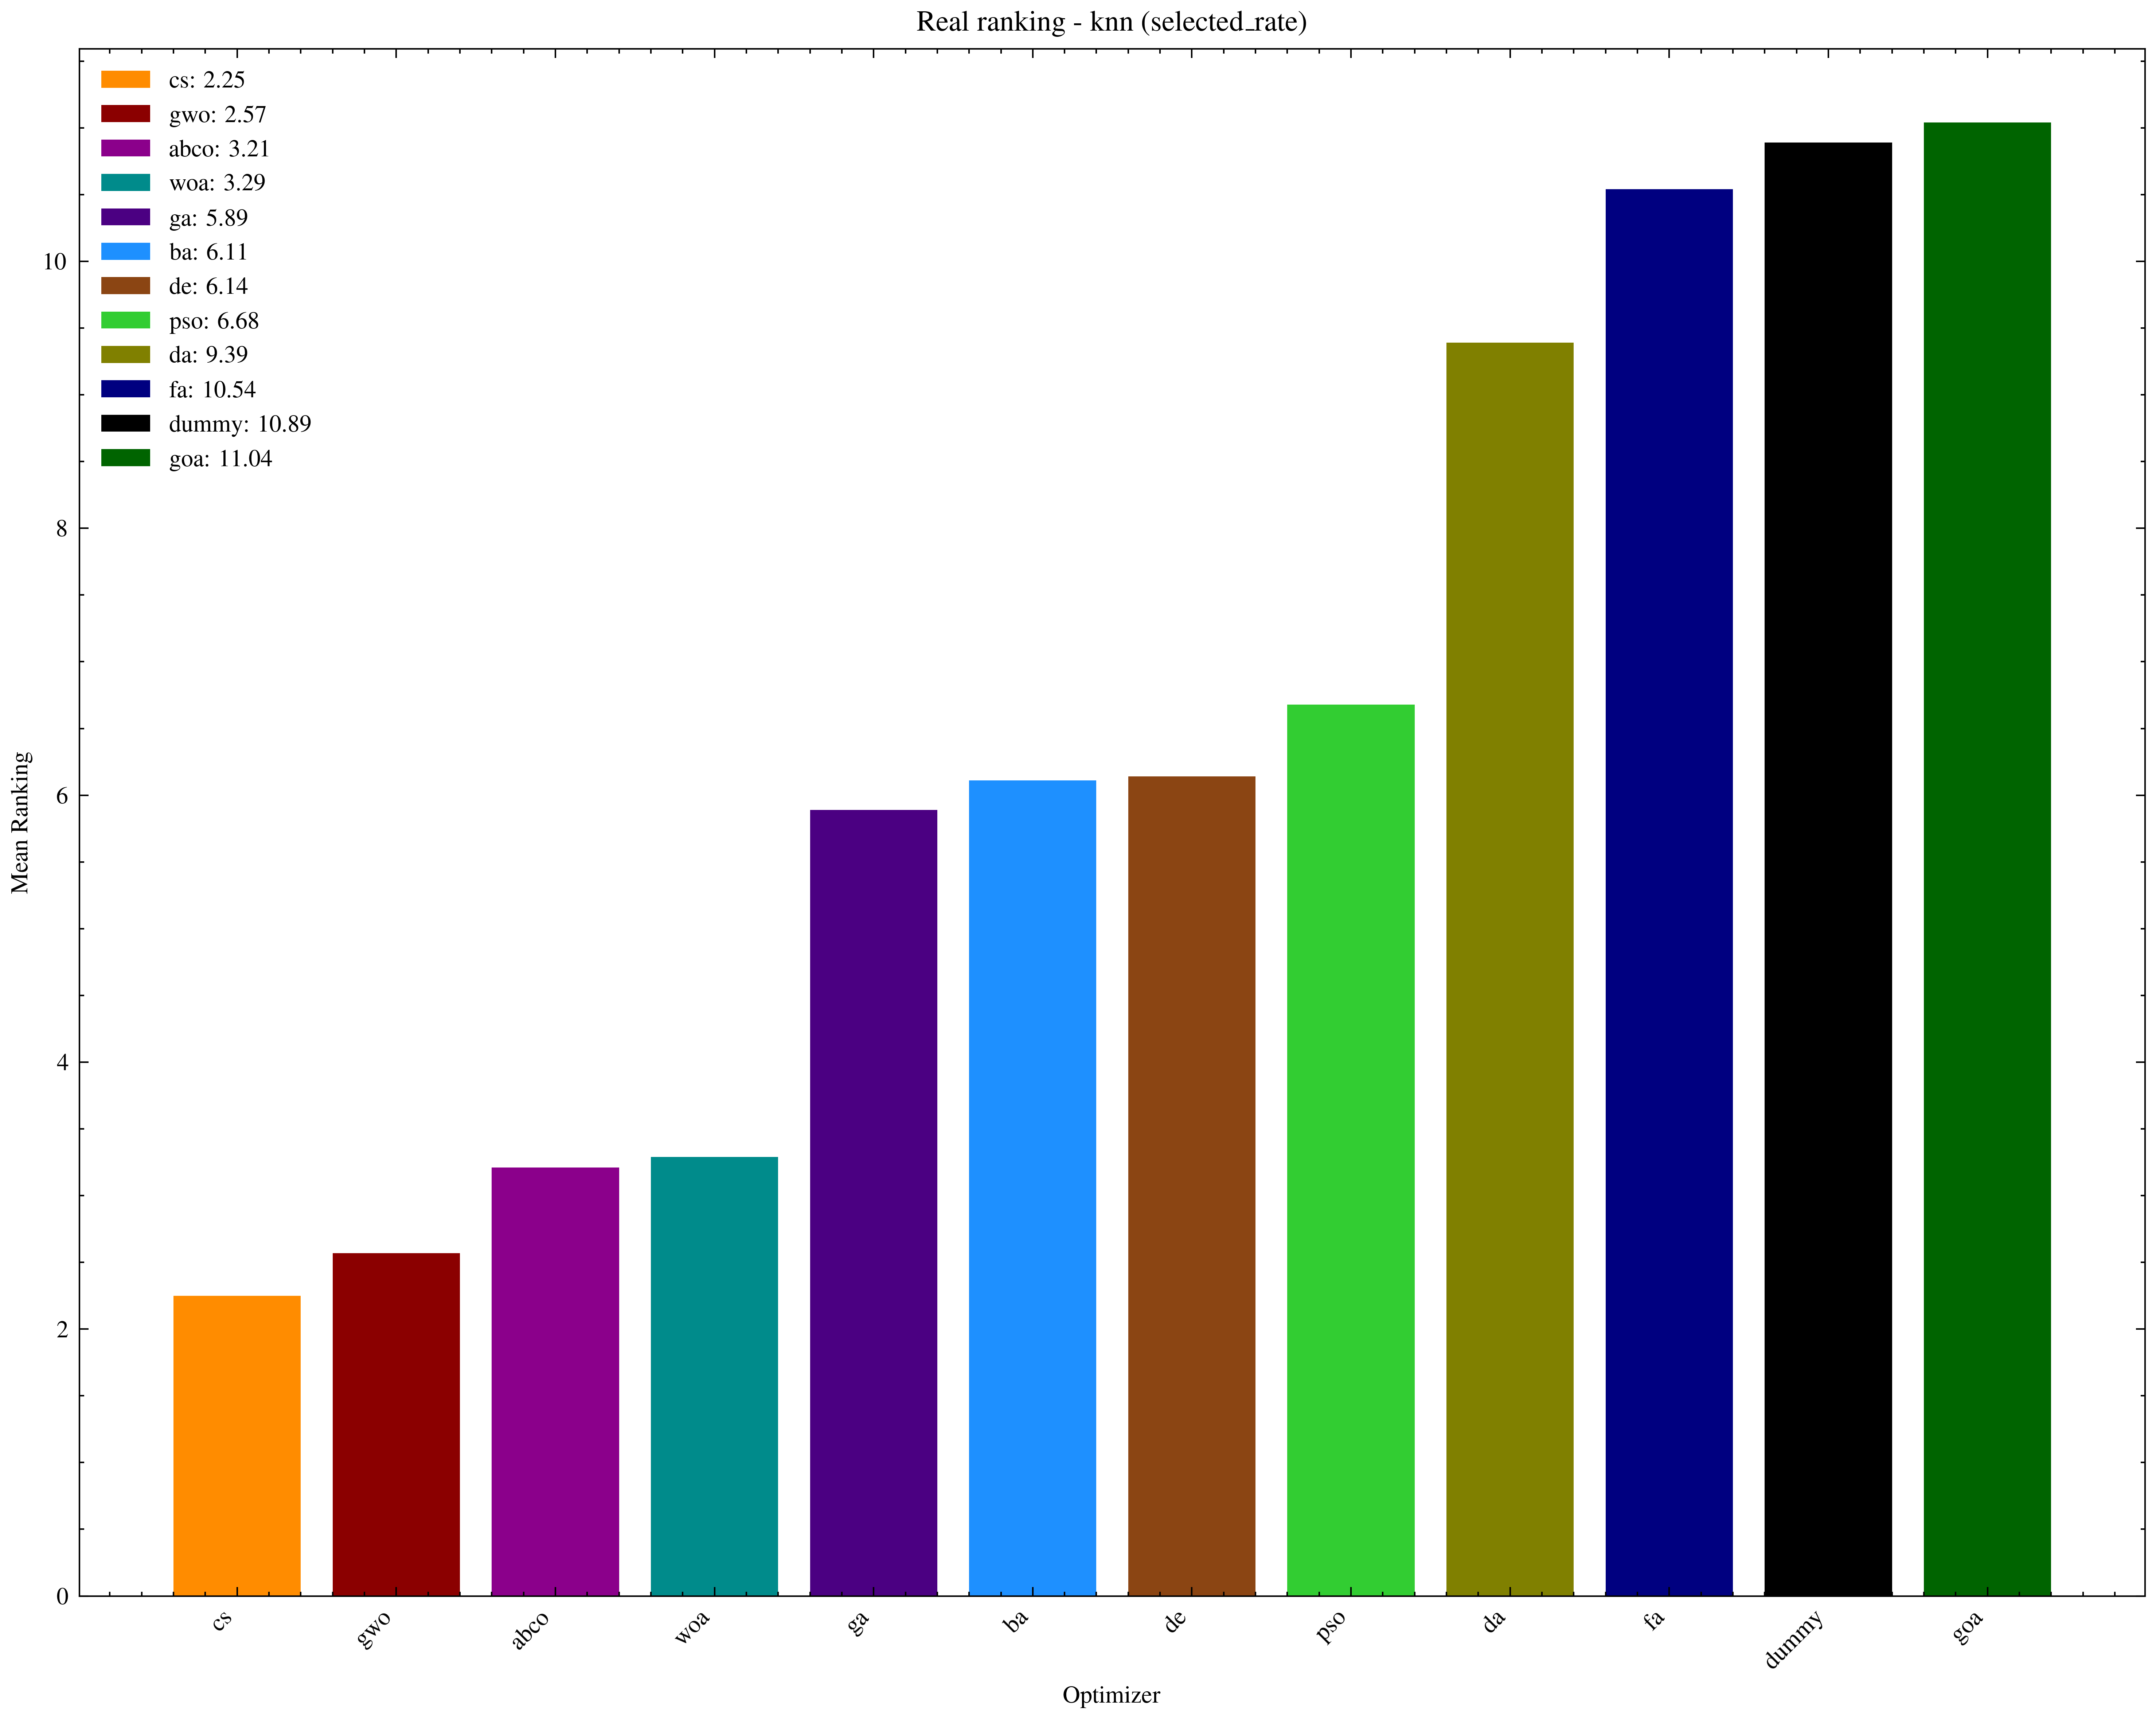
\includegraphics[width=\textwidth]{imagenes/fitness_charts/img/binary/rankings_knn_selected_rate.png}
        \caption{Ranking por ratio de reducción para knn}
        \label{fig:ranking_knn_red}
    \end{subfigure}
    \begin{subfigure}[b]{1\textwidth}
        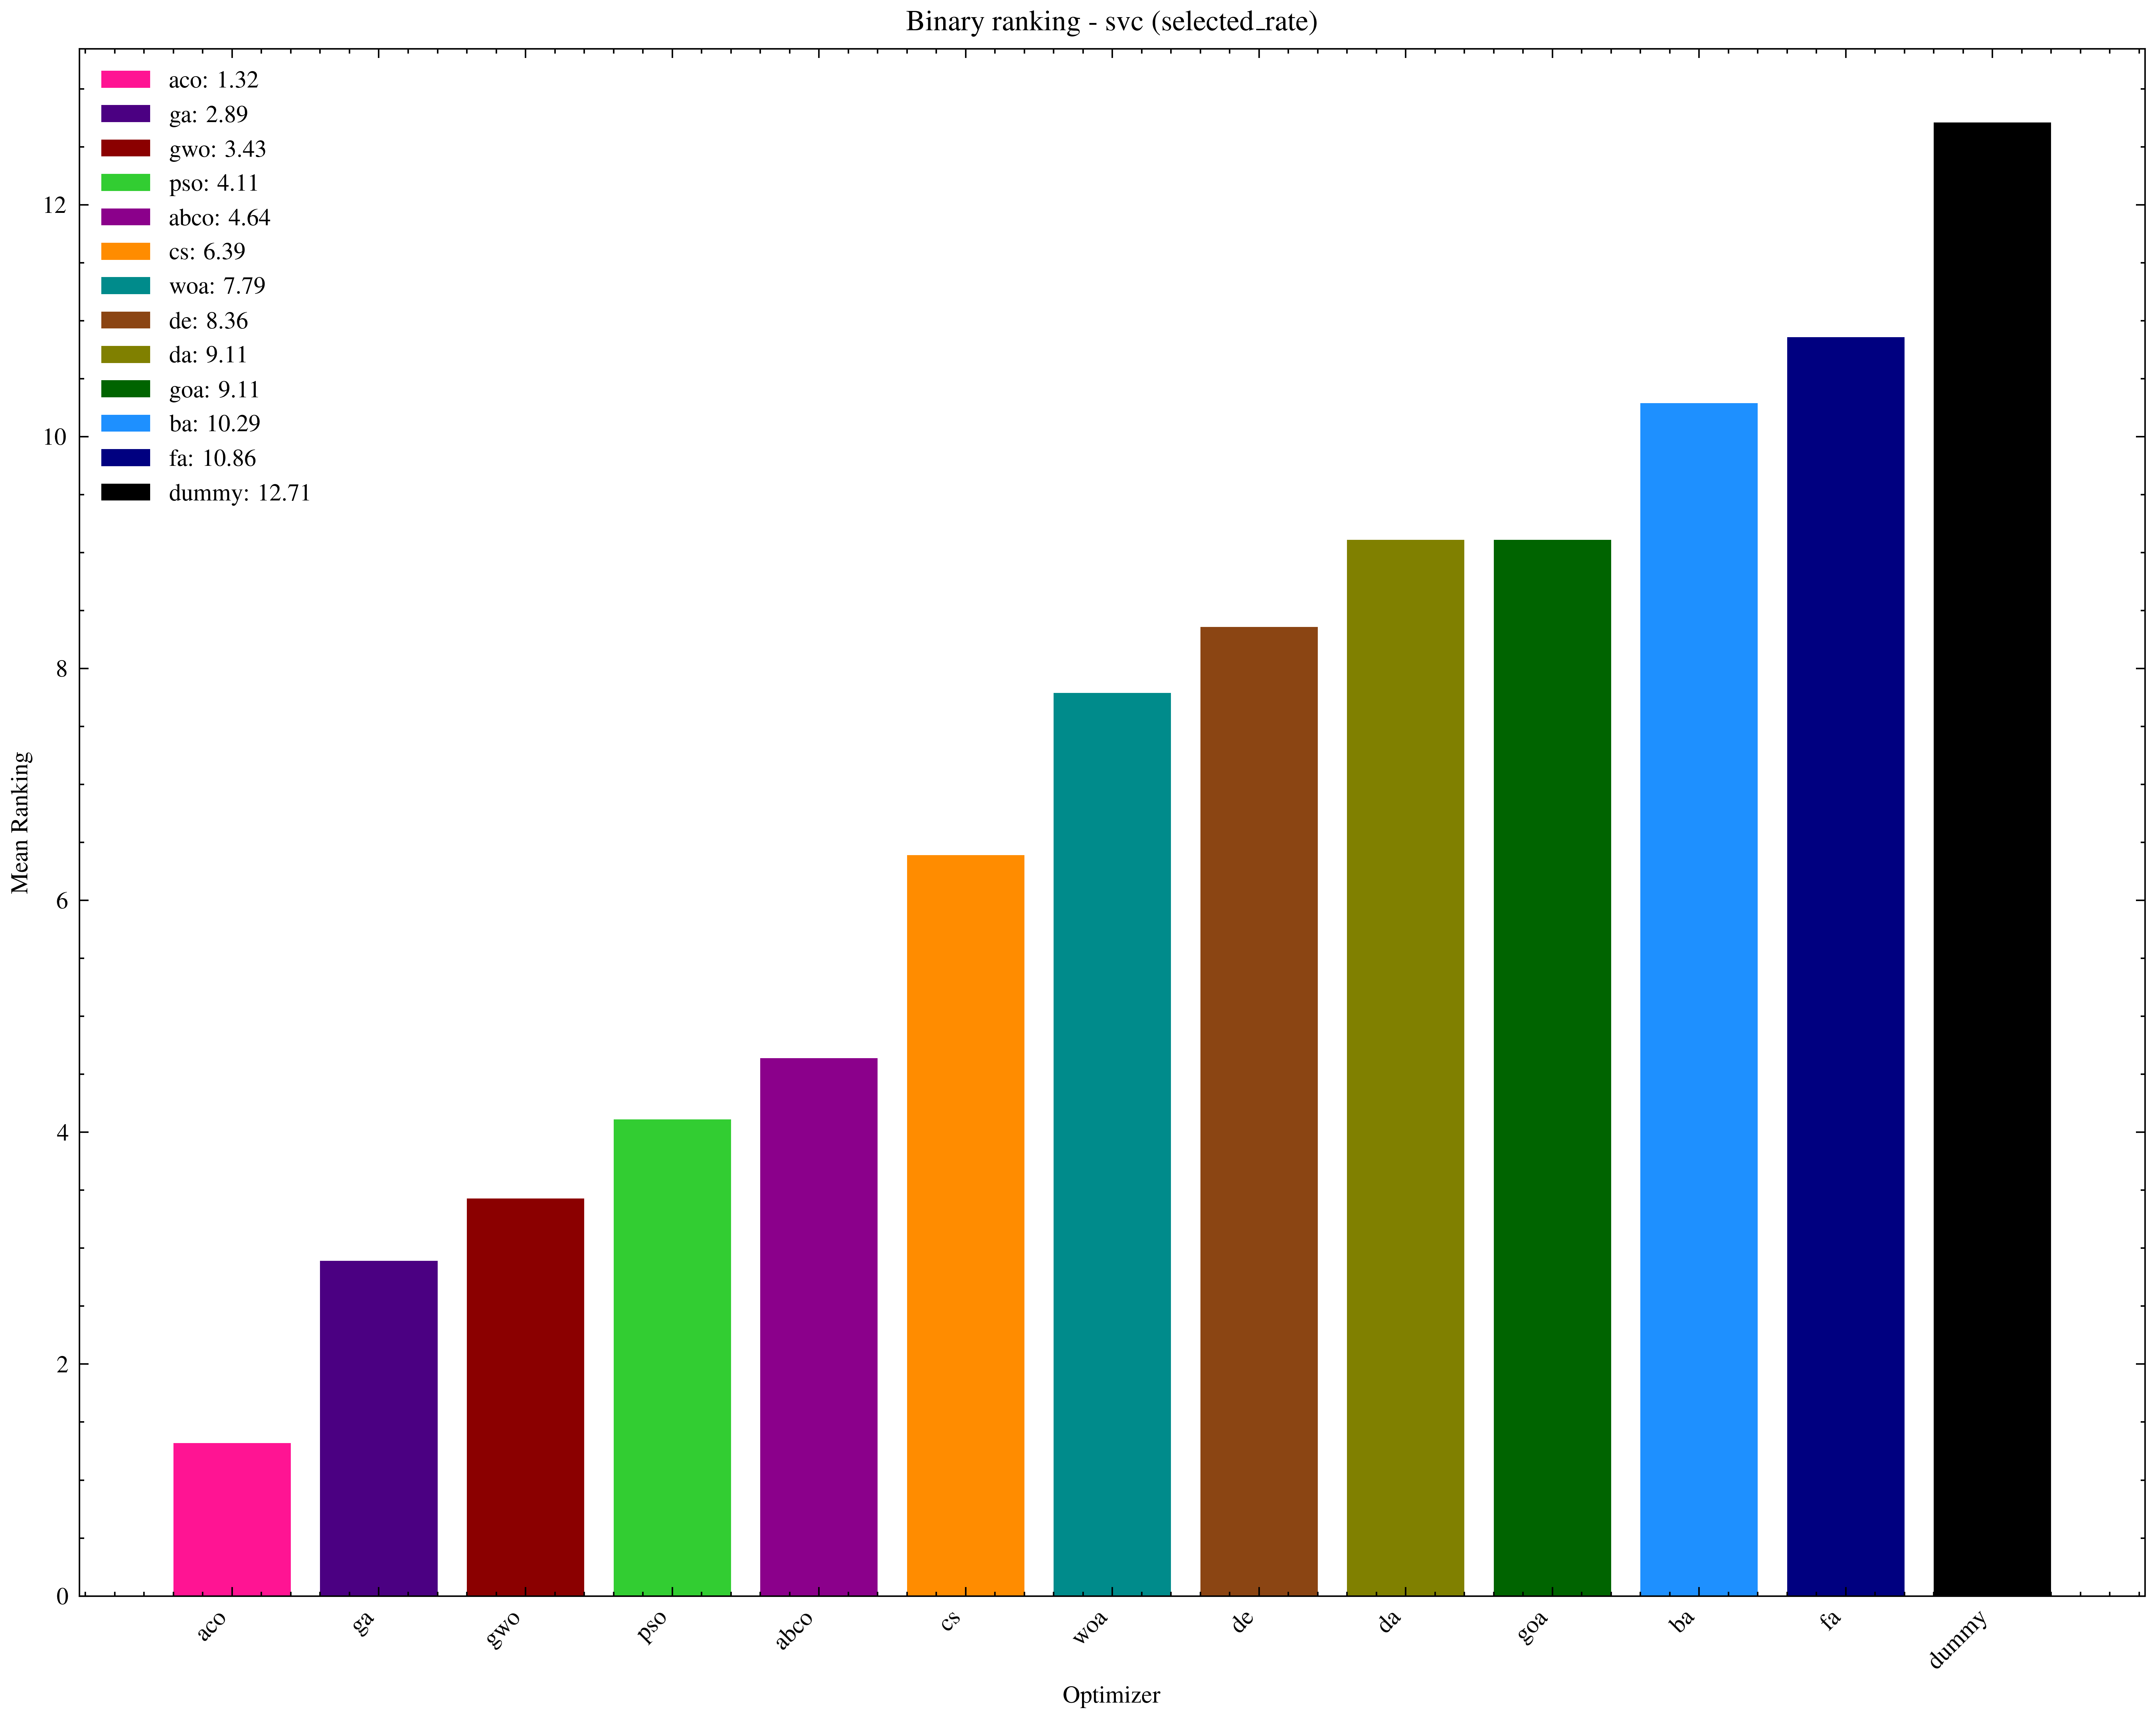
\includegraphics[width=\textwidth]{imagenes/fitness_charts/img/binary/rankings_svc_selected_rate.png}
        \caption{Ranking por ratio de reducción para svc}
        \label{fig:ranking_svc_red}
    \end{subfigure}
    \caption{Rankings para reducción de características}
    \label{fig:rankings_red}
\end{figure}

Por tanto tanto un grupo como otro parece alcanzar resultados bastante satisfactorios en este sentido.

En cuanto a la reducción de características, según se observa en los rankings \ref{fig:rankings_red} como \textbf{ACO} es sin duda el mejor, por mucho además. Es capaz de reducir en algunos casos hasta el $90\%$ de las características.\\[6pt]
Si se observan los p-valores obtenidos en la tabla \ref{tab:p-values_red} y se agrupan los modernos y los clásicos, se obtienen los siguientes resultados:
\begin{itemize}
    \item \textbf{bPSO}: A excepción del \textbf{ACO} (el mejor), \textbf{bGWO} (segundo mejor) y \textbf{bGA}, es superior a todo el resto de algoritmos con una diferencia significativa más que suficiente, incluso tras corrección post hoc con el método \textbf{Holms}.
    \item \textbf{ACO}: Es el mejor con diferencia significativa más que suficiente como para poder afirmar que este algoritmo es muy destacable en la reducción de características.
    \item \textbf{bGA}: Ocurre lo mismo que con \textbf{bPSO}. Pese a excepciones de algoritmos por encima suyo en el ranking, \textbf{bGA} es muy superior al resto de algoritmos, con diferencias muy notables y de nuevo significativas.
    \item \textbf{bDE}: Obtiene resultados muy buenos y estadísticamente significativos con respecto a \textbf{bBA}, \textbf{bWOA} y \textbf{bFA}. Pese a ser mejor que otros algoritmos modernos, la diferencia no es suficientemente como para rechazar la hipótesis nula.
    \item \textbf{bABCO}: El peor parado del grupo de los algoritmos clásicos. No parece ser una buena propuesta a la hora de reducir.
\end{itemize}

Dada estos resultados, los algoritmos clásicos salen muy bien parados en la reducción de características frente a los modernos. Si bien es cierto que hay dos algoritmos que destacan sobre el resto de los modernos (\textbf{bCS} y \textbf{bGWO}) en la reducción de características, los clásicos en conjunto, con excepción de \textbf{bABCO}, parecen una opción robusta y que, en combinación a sus resultados de precisión (\textit{accuracy}), son muy precisos a la hora de seleccionar características importantes.

\subsubsection{Mejor vs Segundo mejor}
Como se ha mencionado anteriormente, la metaheurística \textbf{ACO} es sin lugar a dudas la mejor.
Un ejemplo de esto es en el conjunto de datos de \textit{ionosphere}. Se puede observar como el segundo algoritmo que más reduce, que es \textbf{bGWO}, obtiene una reducción media del $74\%$, mientras que el \textbf{ACO} obtiene una reducción media del $91.5\%$, con tan solo una diferencia de $4.6\%$ en precisión a favor de \textbf{bGWO}~\ref{tab:bin_red_acc_all}. \\[6pt]
Si bien es cierto que su precisión no es de las mejores, se mantiene en mitad de los rankings con el resto de algoritmos. Teniendo ese aspecto en cuenta, añadido a que es capaz de reducir características a un nivel muy significativo con respecto al resto de algoritmos, \textbf{ACO} se presenta como un algoritmo muy interesante para aquellos problemas en los que se pueda permitir cierto nivel de error en la precisión, pero en cambio, sea crucial una compresión del tamaño del modelo o un tiempo den entrenamiento corto.\\[6pt]

Si comparamos los p-valores~\ref{tab:p-values_aco_rest}, tras aplicar post hoc para mayor seguridad, de \textbf{ACO} con respecto al resto de algoritmos, se ve que claramente la mejora en reducción no se debe al azar de manera muy probable.

\subsubsection{bWOA vs bGWO}
Dentro del conjunto de algoritmos analizados, hay ciertos pares que resultan interesantes por la semejanza algorítmica e inspirativa entre ambos. En esta sección, se compararán los algoritmos \textbf{bWOA} y \textbf{bGWO}. Ambos pertenecen a la categoría de algoritmos de optimización inspirados en la naturaleza y ambos se inspiran fuertemente en el comportamiento social y estrategias de caza de ciertos animales.\\[6pt]
Dentro del contexto de la caza, tanto \textbf{WOA} como \textbf{GWO} utilizan ecuaciones que simulan el rodeo de la presa, aunque con diferencias en la implementación y el comportamiento específico. A continuación se detallan los comportamientos de rodeo de la presa en la caza:
\begin{itemize}
    \item \textbf{bWOA}: La ballena ajusta su posición no solo moviéndose hacia la presa sino también rodeándola en un patrón circular, lo cual le permite cubrir más área y ajustar su aproximación con mayor precisión. La espiral seguida en la fórmula depende del parámetro de control $D$.
    \item \textbf{bGWO}: Los lobos rodean a la presa en grupos liderados por alfa, beta y delta. Al reducir la distancia a estas posiciones líderes, los lobos de menor rango simulan el cerco y convergen hacia la presa de manera cooperativa. El acercamiento utiliza un vector de coeficientes $A$ que decrece linealmente.
\end{itemize}

Ambos algoritmos por tanto, y pese a sus diferencias, comparten una naturaleza y comportamiento parecido a la hora buscar soluciones. Al comparar ambos resultados en \textbf{accuracy}, se aprecia que estos no difieren de manera suficiente en su rendimiento como para poder rechazar la hipótesis nula. Véase en la tabla \ref{tab:p-values_accuracy}\\[6pt]

Es en cambio en la comparación en la métrica de reducción de características donde se ve que \textbf{bGWO} presenta una diferencia notable con respecto a \textbf{bWOA}. Puede observarse gráficamente en las figuras \ref{fig:svc_selected_rate_gwo_woa_bin} como \textbf{bWOA} reduce considerablemente menos que \textbf{bGWO}. Comprobarse también que las diferencias entre ambos son estadísticamente significativas \ref{tab:pval_corr_gwo_woa-bin}

\begin{table}[htb]
    \centering
    \begin{tabular}{lllll}
        \toprule
        {}       & Original & Holm           & Hommel         & Hochberg       \\
        \midrule
        woa\_knn & 0.001    & \textbf{0.003} & \textbf{0.002} & \textbf{0.002} \\
        woa\_svc & 0.001    & \textbf{0.003} & \textbf{0.002} & \textbf{0.002} \\
        gwo\_svc & 0.028    & \textbf{0.028} & \textbf{0.028} & \textbf{0.028} \\
        \bottomrule
    \end{tabular}
    \caption{P-valores tras corrección entre bGWO-kNN y demás algoritmos en reducción de características}
    \label{tab:pval_corr_gwo_woa-bin}
\end{table}

Incluso la versión de \textbf{bGWO} que utiliza \textit{kNN} es significativamente más discriminativa con las características seleccionadas que su versión con \textbf{SVC}.

\begin{figure}[htb]
    \centering
    \begin{subfigure}[b]{0.45\textwidth}
        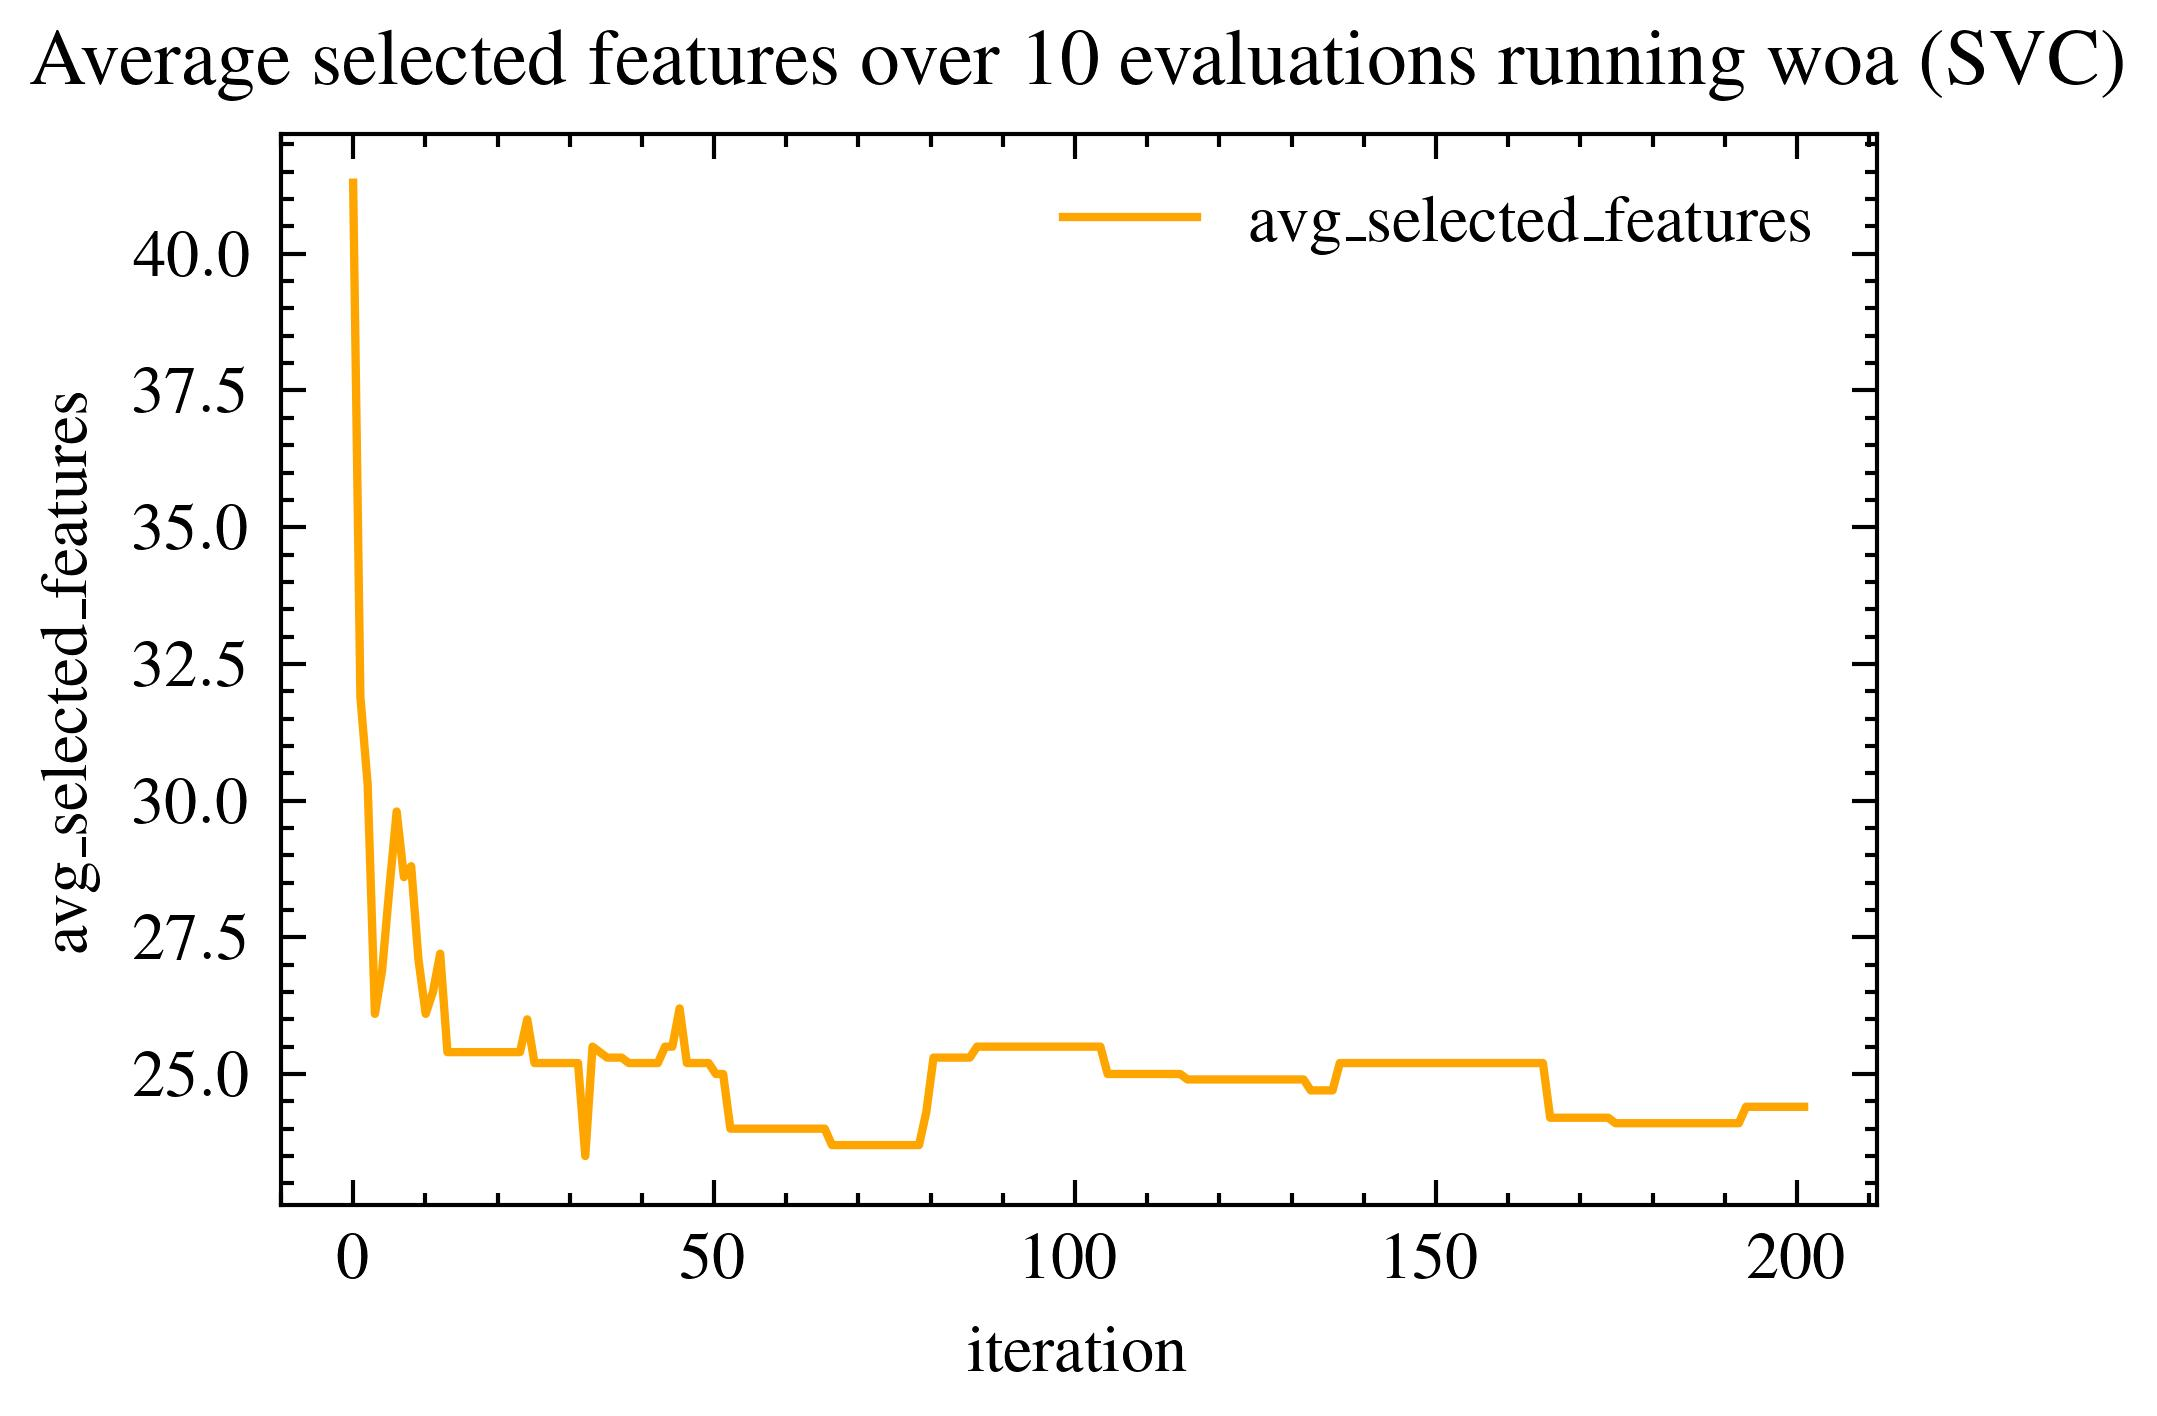
\includegraphics[width=\textwidth]{imagenes/fitness_charts/img/binary/spectf-heart/SVC_n_features_over_10_evaluations_woa_binary_spectf-heart.jpg}
        \caption{spectf-heart}
    \end{subfigure}
    \begin{subfigure}[b]{0.45\textwidth}
        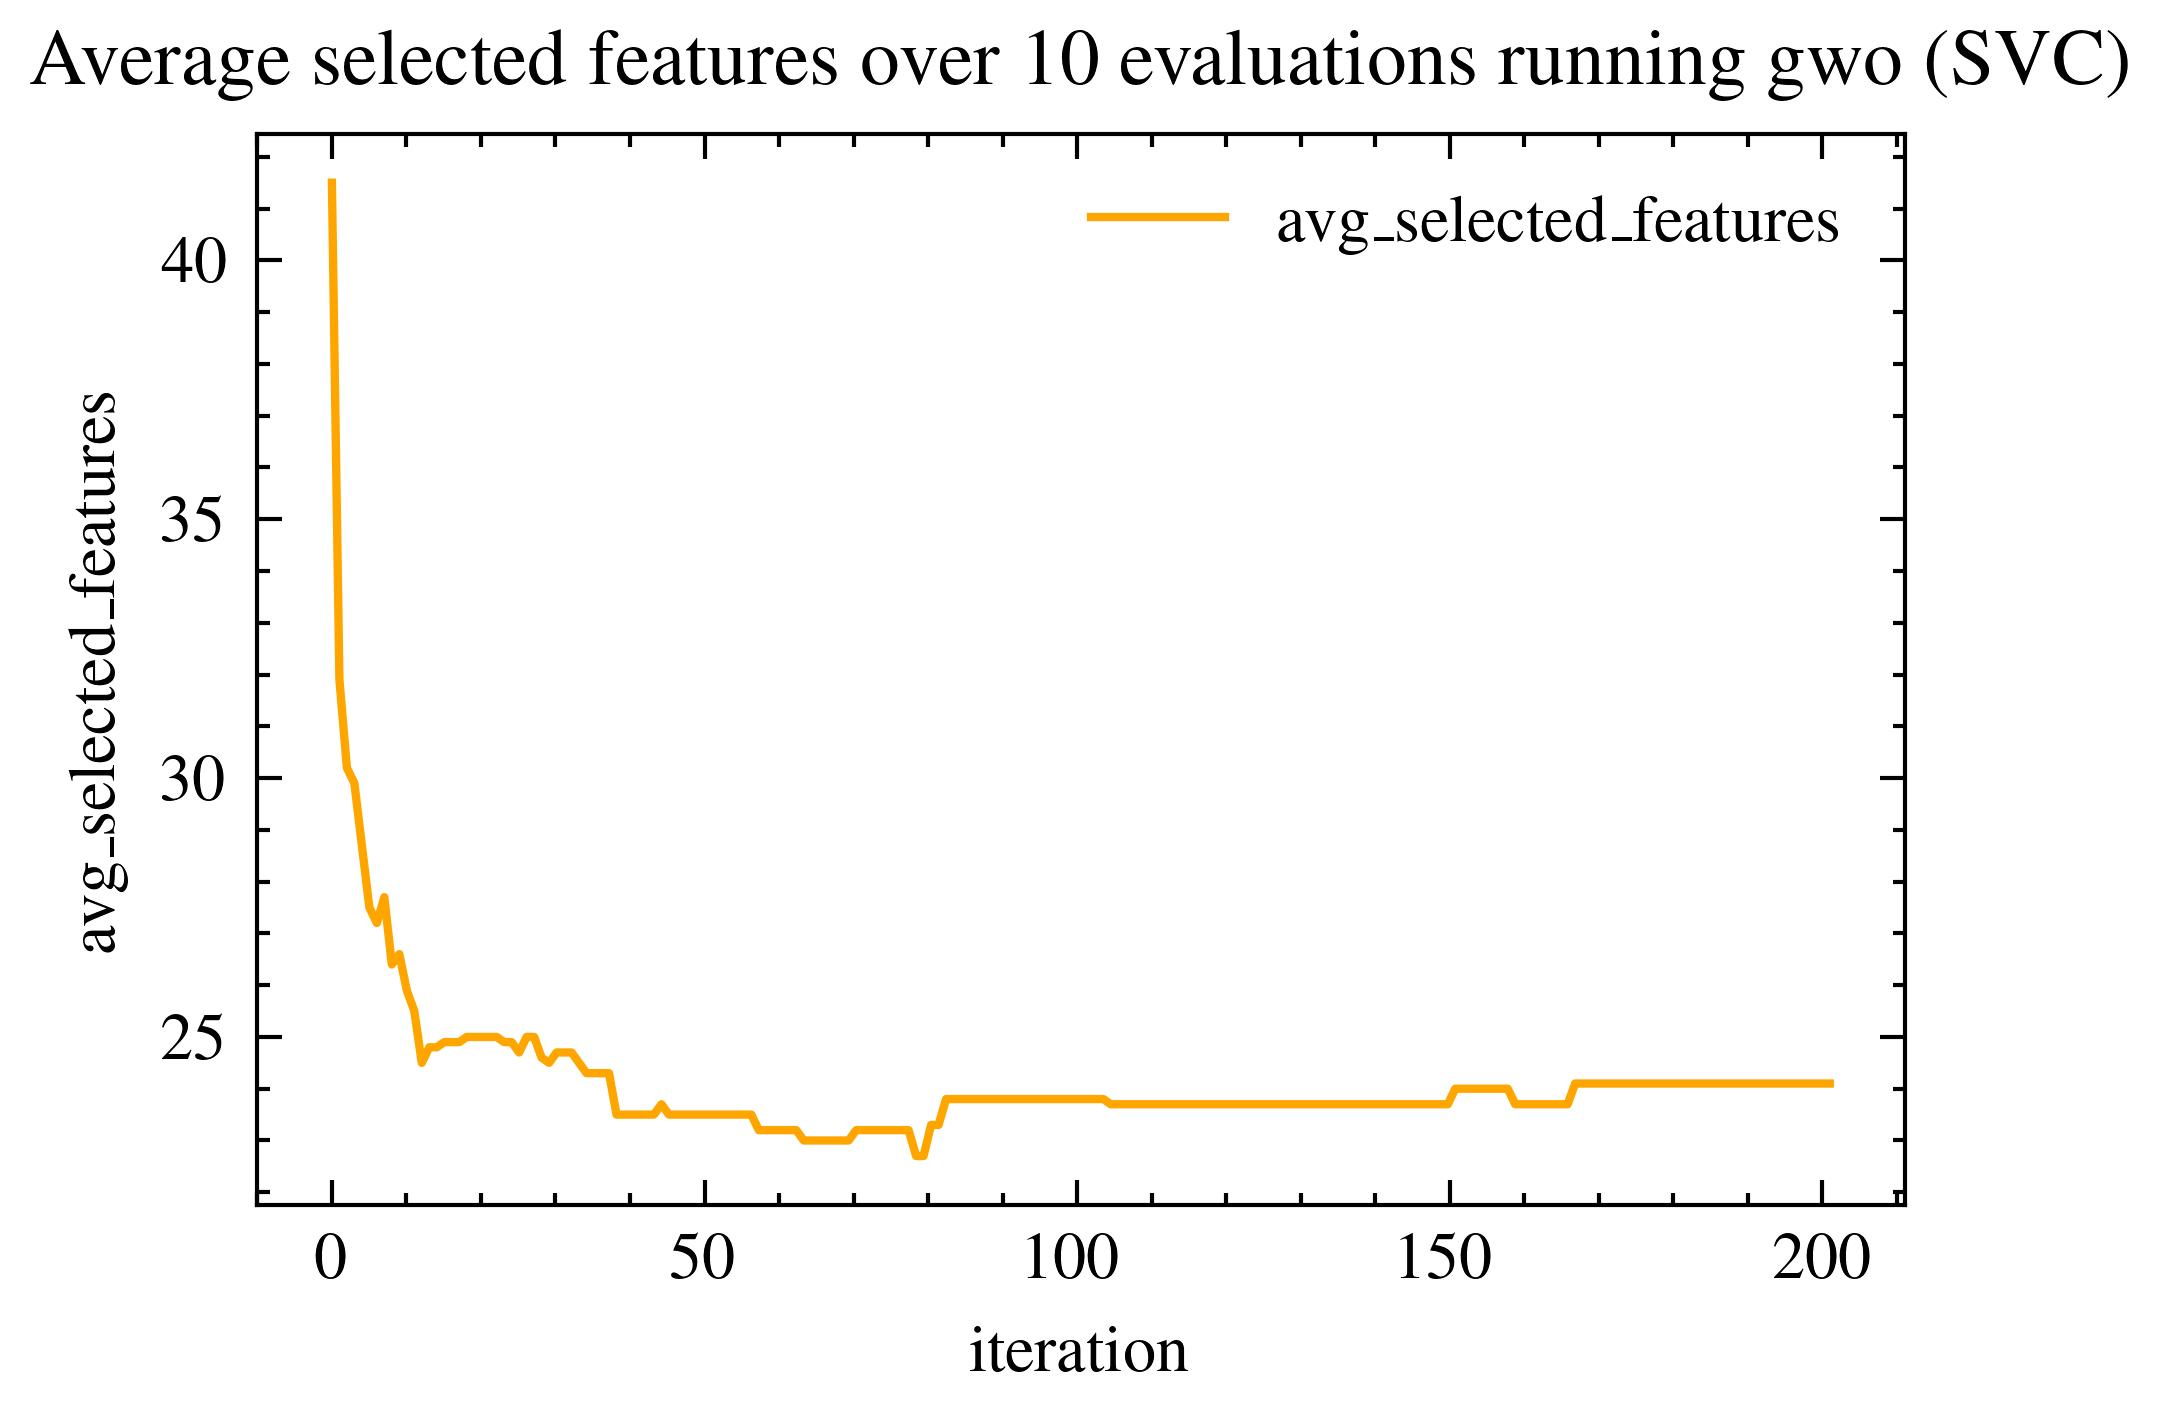
\includegraphics[width=\textwidth]{imagenes/fitness_charts/img/binary/spectf-heart/SVC_n_features_over_10_evaluations_gwo_binary_spectf-heart.jpg}
        \caption{spectf-heart}
    \end{subfigure}

    \begin{subfigure}[b]{0.45\textwidth}
        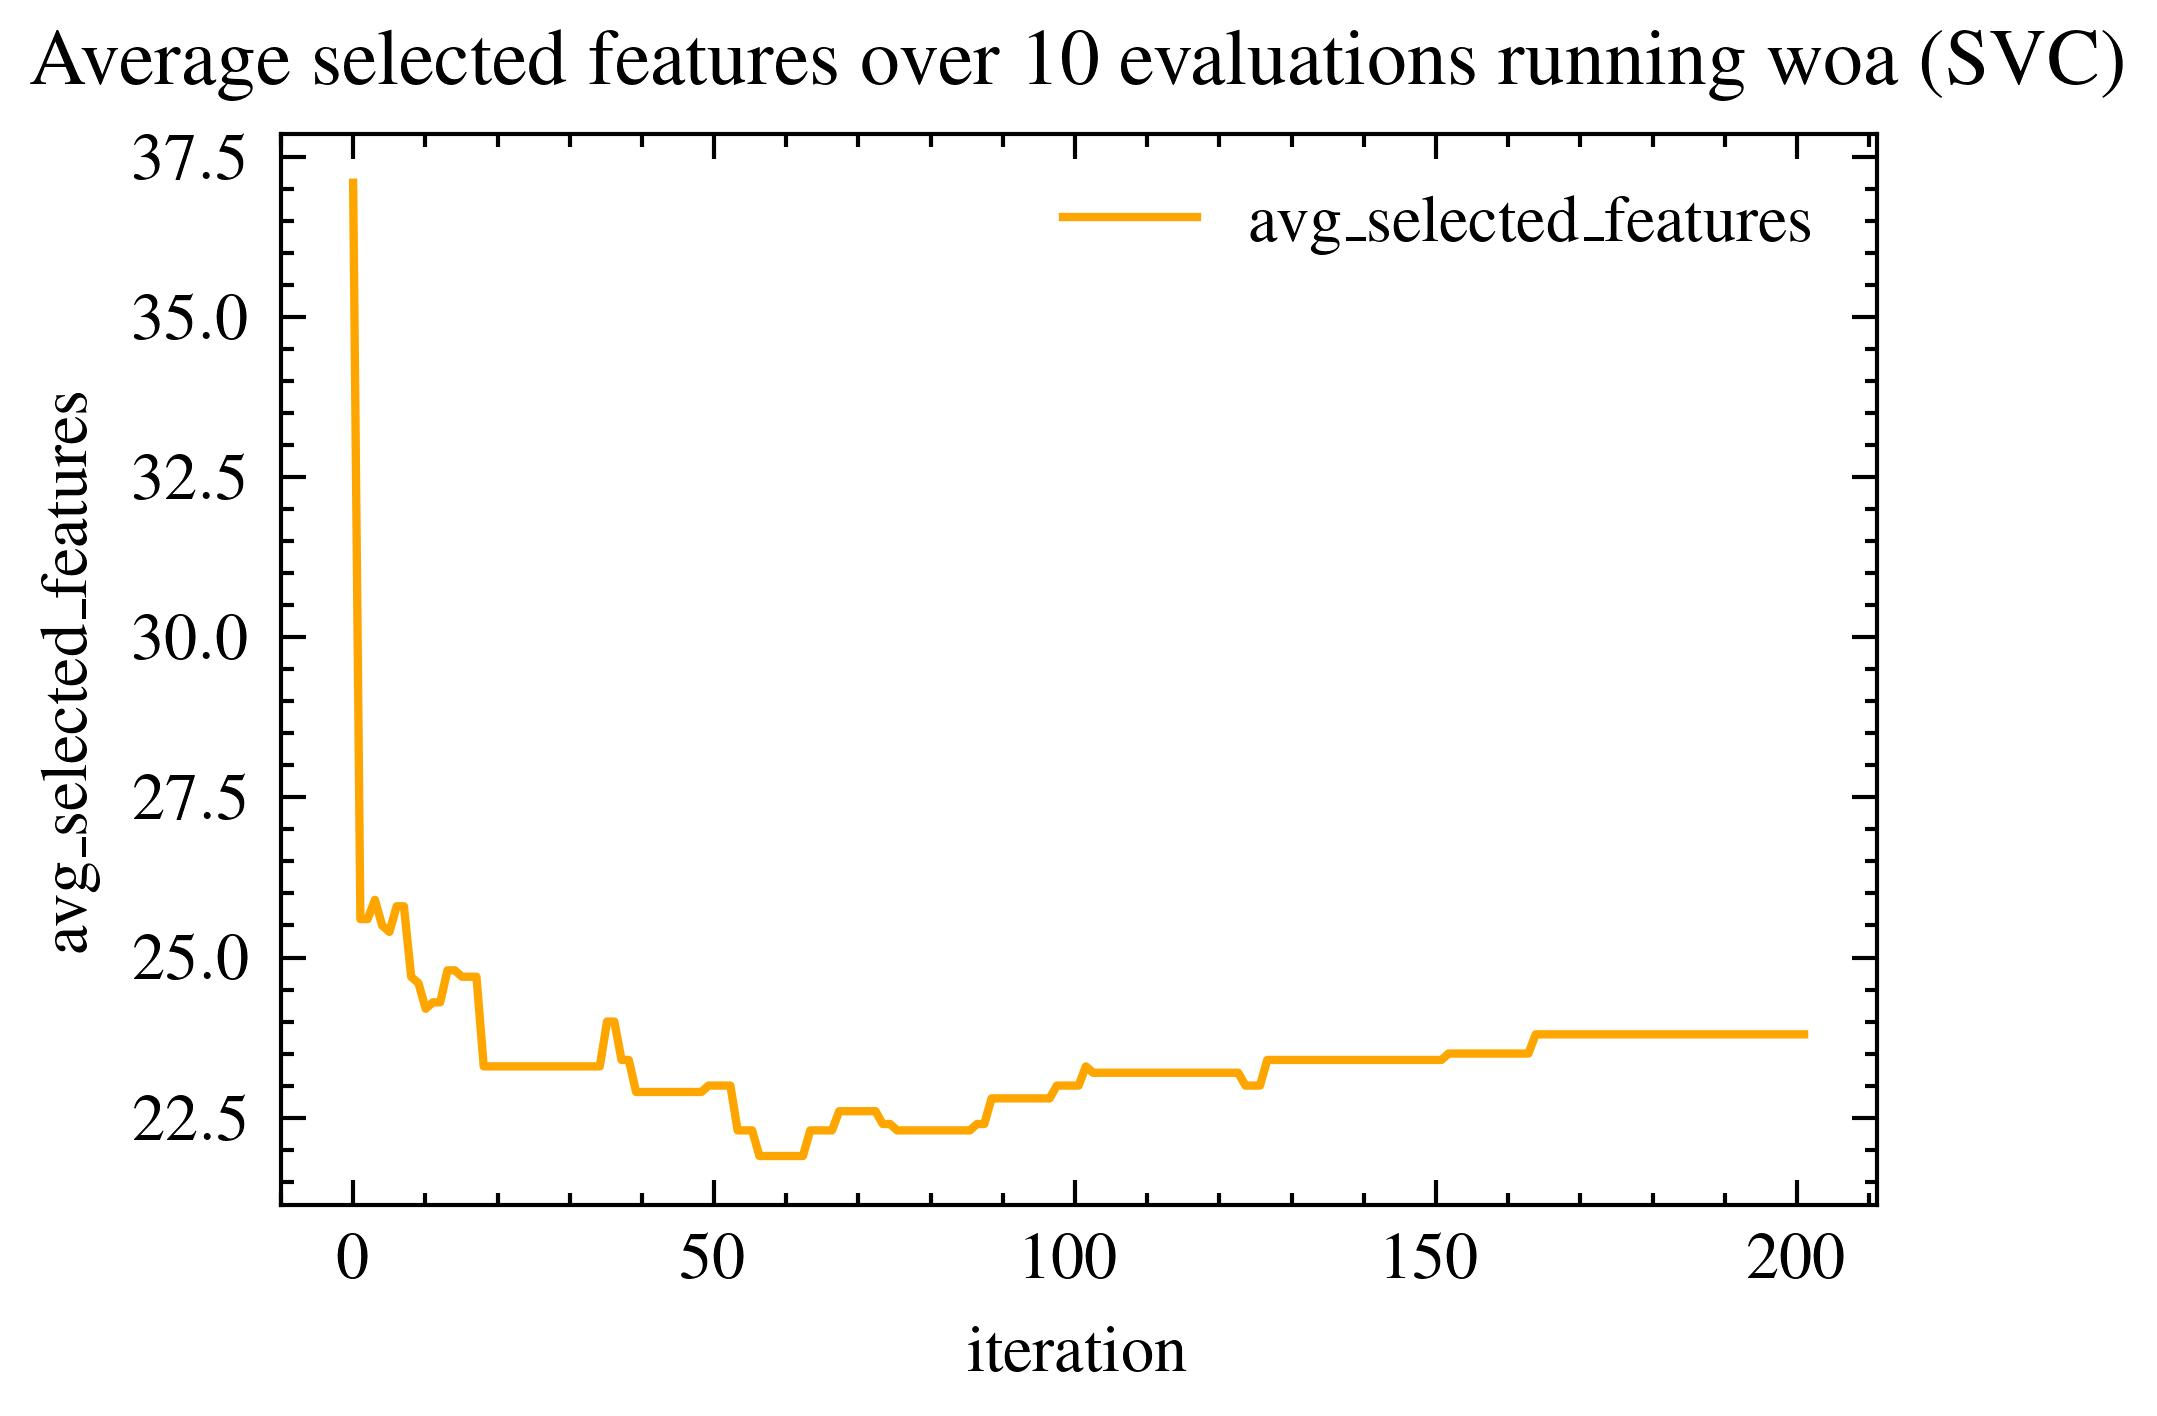
\includegraphics[width=\textwidth]{imagenes/fitness_charts/img/binary/waveform5000/SVC_n_features_over_10_evaluations_woa_binary_waveform5000.jpg}
        \caption{waveform5000}
    \end{subfigure}
    \begin{subfigure}[b]{0.45\textwidth}
        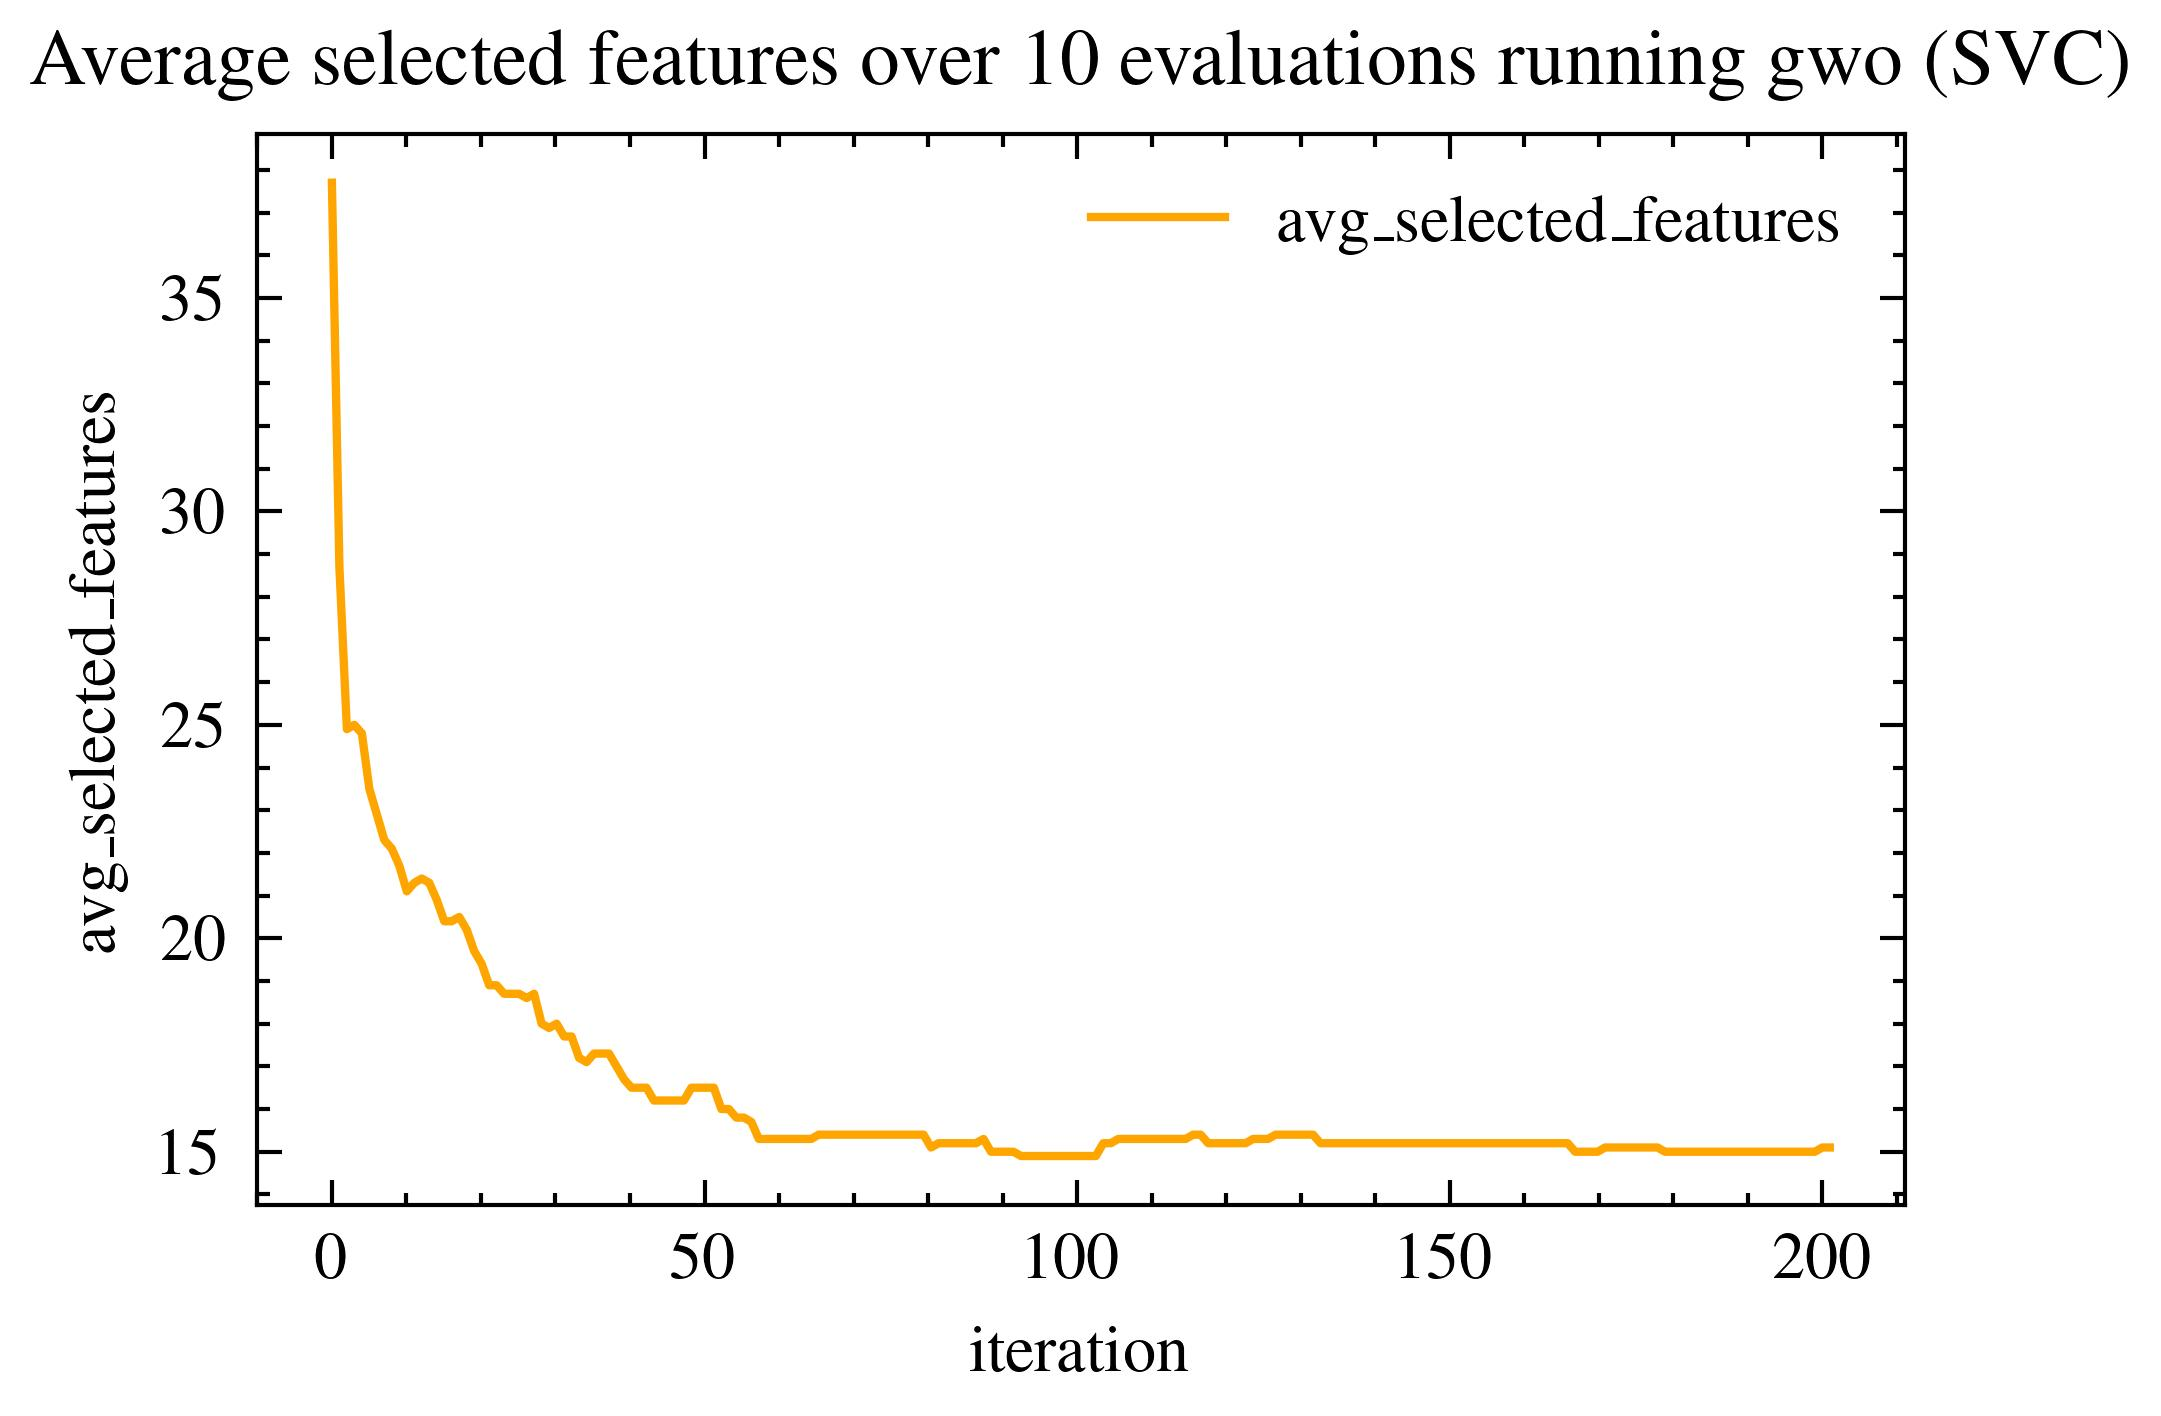
\includegraphics[width=\textwidth]{imagenes/fitness_charts/img/binary/waveform5000/SVC_n_features_over_10_evaluations_gwo_binary_waveform5000.jpg}
        \caption{waveform5000}
    \end{subfigure}

    \begin{subfigure}[b]{0.45\textwidth}
        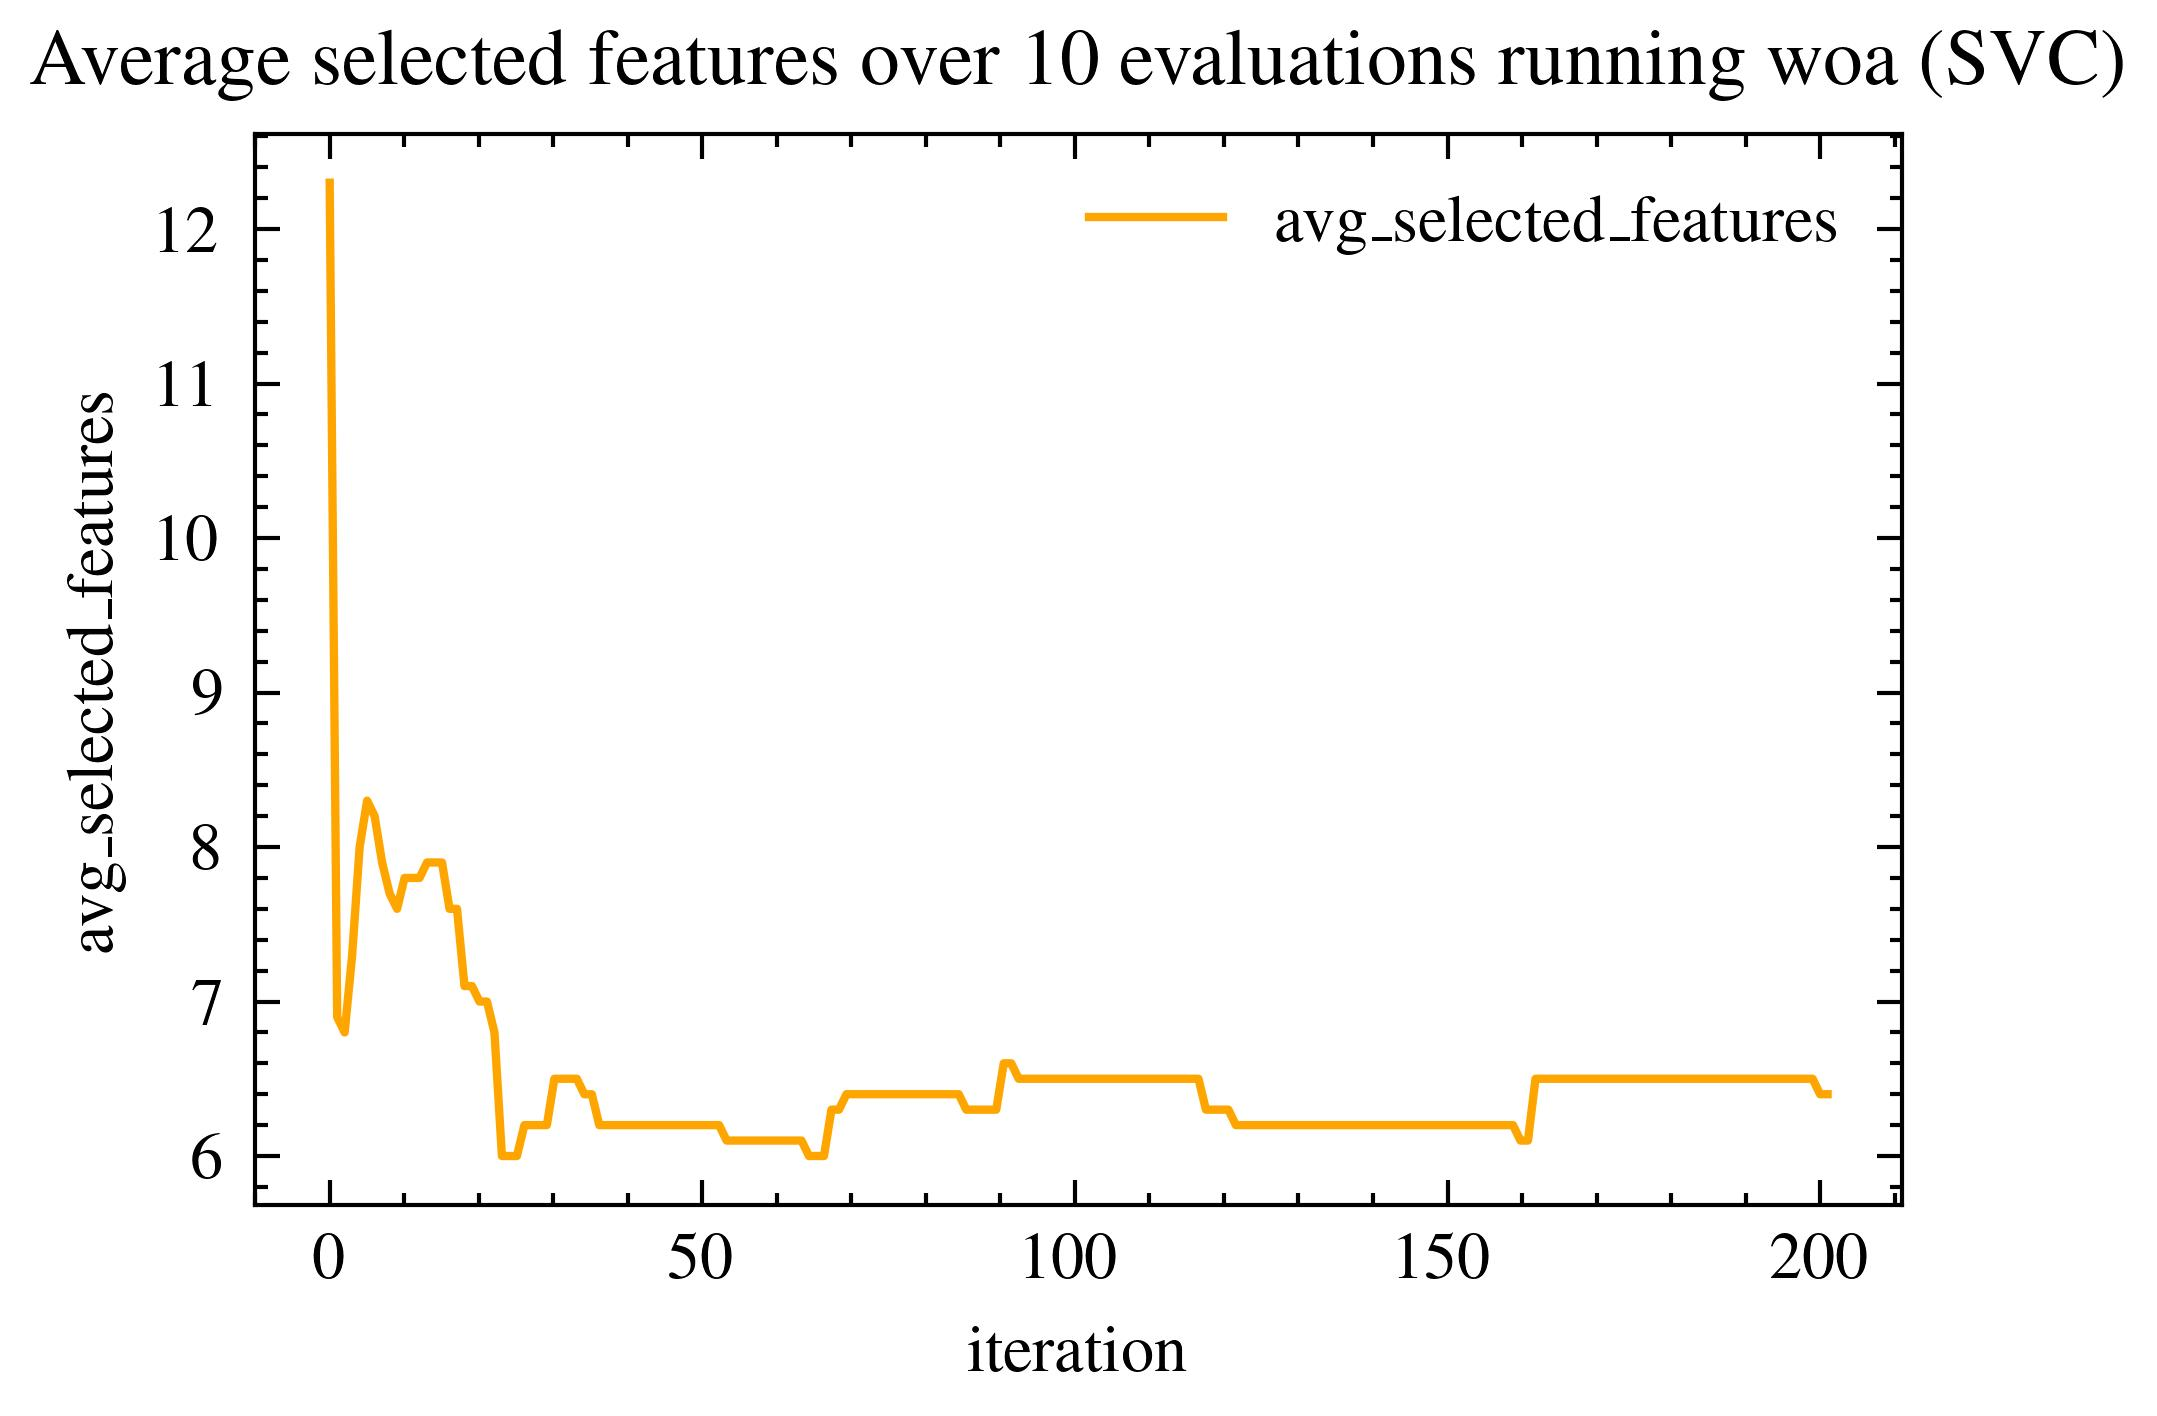
\includegraphics[width=\textwidth]{imagenes/fitness_charts/img/binary/wine/SVC_n_features_over_10_evaluations_woa_binary_wine.jpg}
        \caption{wine}
    \end{subfigure}
    \begin{subfigure}[b]{0.45\textwidth}
        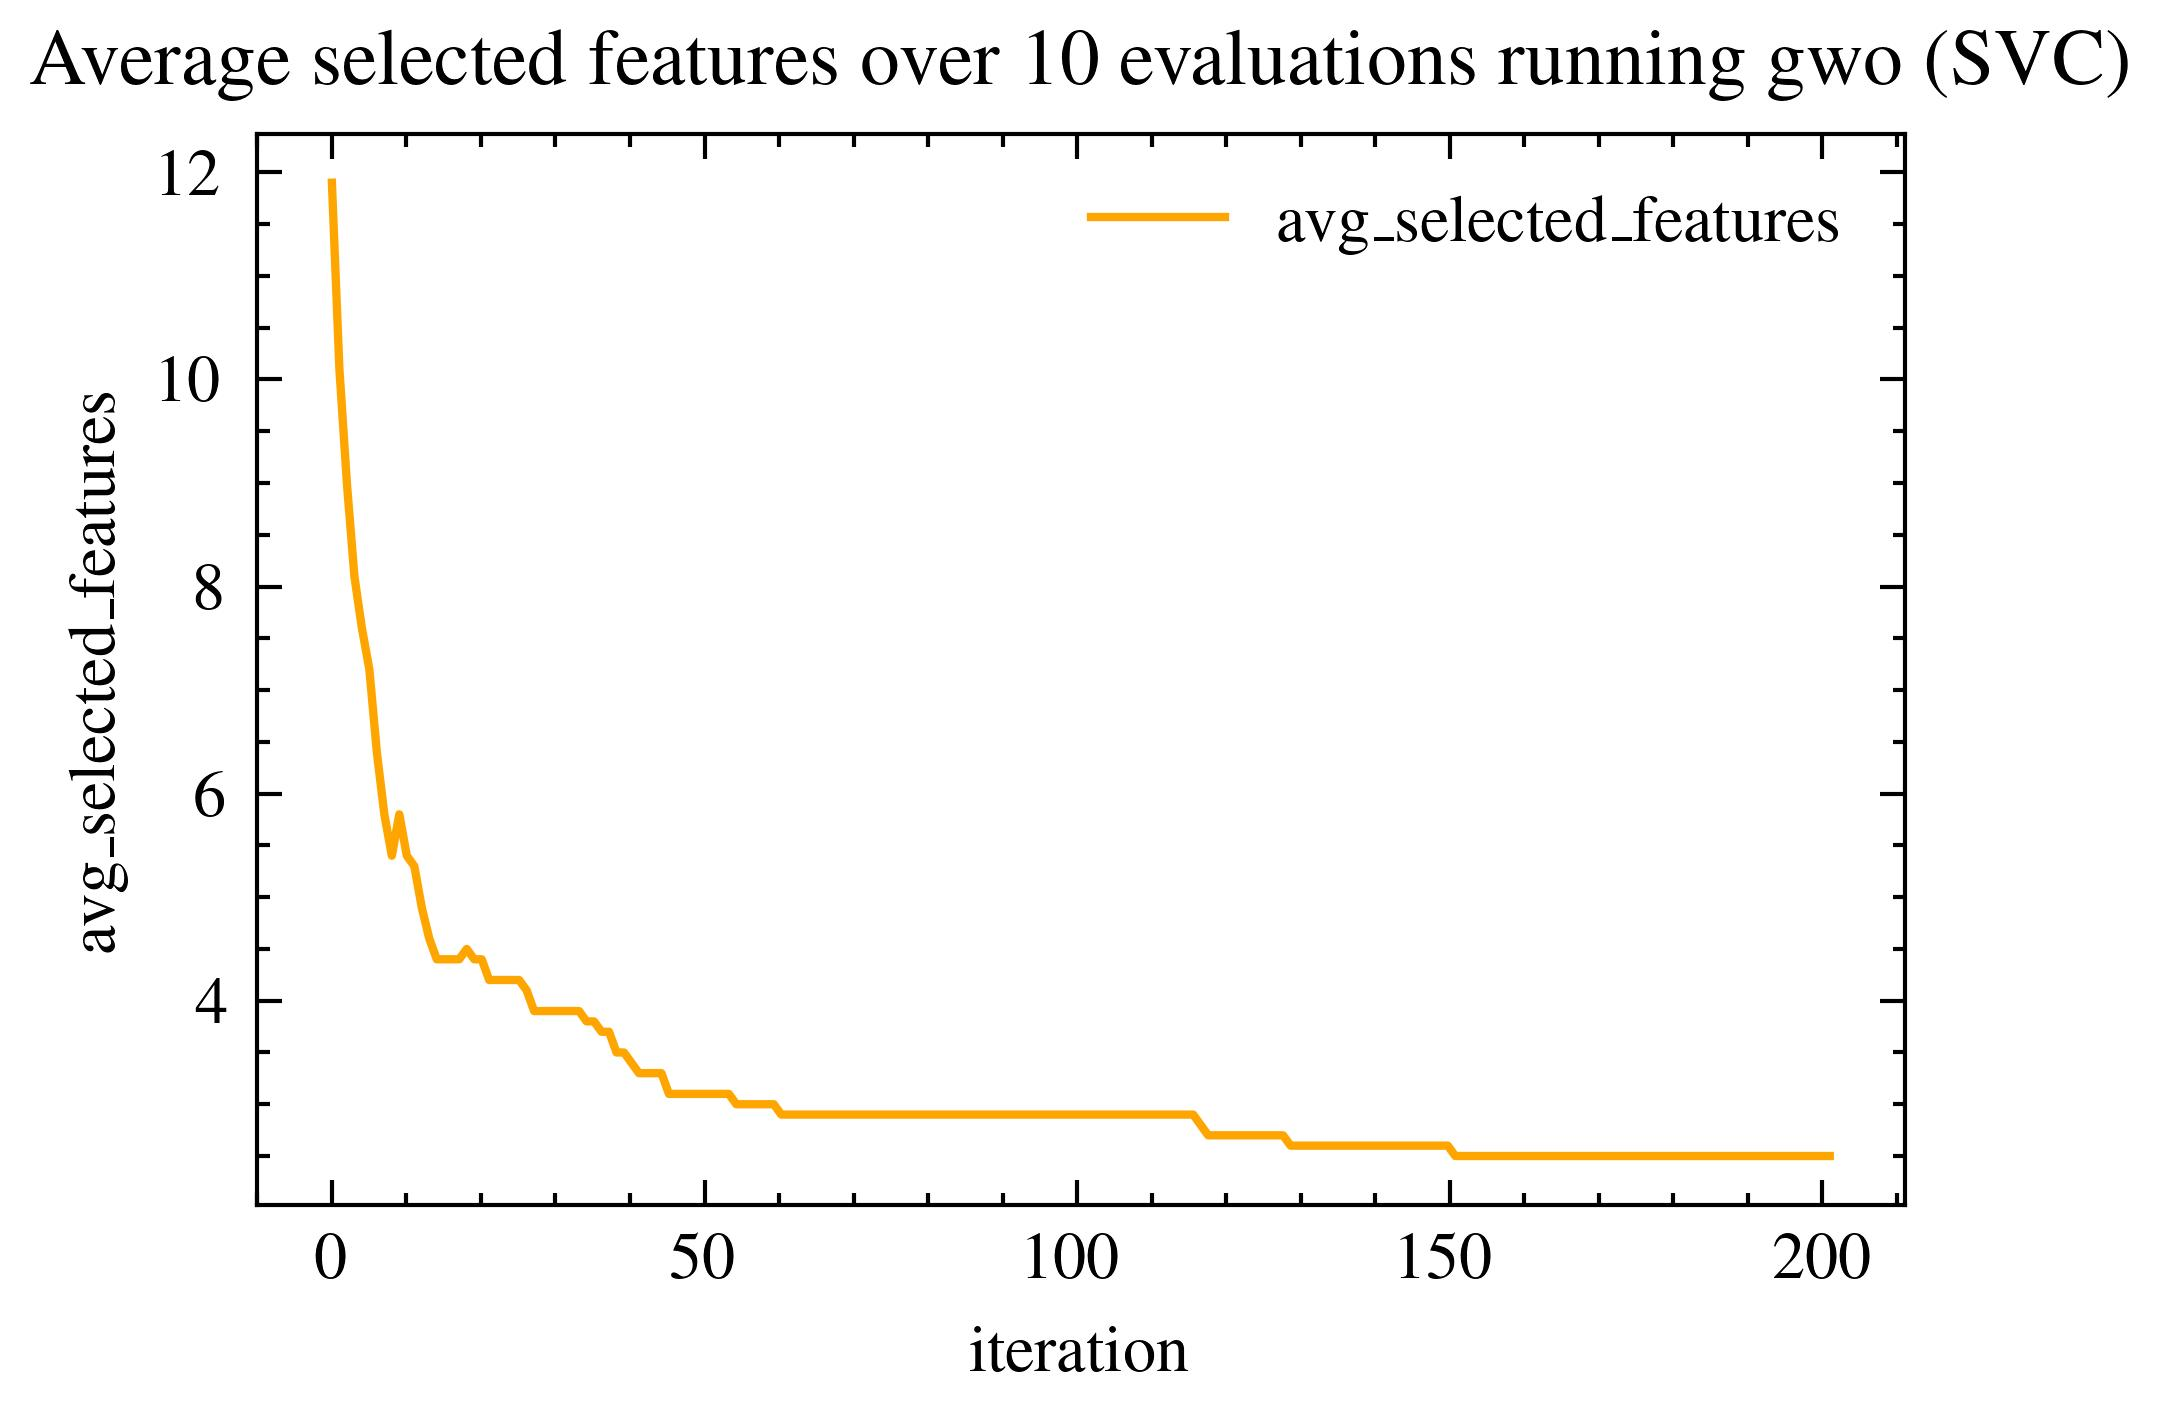
\includegraphics[width=\textwidth]{imagenes/fitness_charts/img/binary/wine/SVC_n_features_over_10_evaluations_gwo_binary_wine.jpg}
        \caption{wine}
    \end{subfigure}

    \caption{Reducción de características en bWOA y bGWO}
    \label{fig:svc_selected_rate_gwo_woa_bin}
\end{figure}

\begin{table}[htb]
    \centering
    \begin{tabular}{lllll}
        \toprule
        {}         & Original  & Holm           & Hommel         & Hochberg       \\
        \midrule
        dummy\_svc & 6.104E-05 & \textbf{0.002} & \textbf{0.001} & \textbf{0.001} \\
        goa\_svc   & 6.104E-05 & \textbf{0.002} & \textbf{0.001} & \textbf{0.001} \\
        goa\_knn   & 6.104E-05 & \textbf{0.002} & \textbf{0.001} & \textbf{0.001} \\
        fa\_knn    & 6.104E-05 & \textbf{0.002} & \textbf{0.001} & \textbf{0.001} \\
        dummy\_knn & 6.104E-05 & \textbf{0.002} & \textbf{0.001} & \textbf{0.001} \\
        fa\_svc    & 0.001     & \textbf{0.014} & \textbf{0.002} & \textbf{0.003} \\
        cs\_svc    & 0.001     & \textbf{0.021} & \textbf{0.002} & \textbf{0.003} \\
        pso\_svc   & 0.001     & \textbf{0.021} & \textbf{0.002} & \textbf{0.003} \\
        pso\_knn   & 0.001     & \textbf{0.021} & \textbf{0.002} & \textbf{0.003} \\
        gwo\_svc   & 0.001     & \textbf{0.021} & \textbf{0.002} & \textbf{0.003} \\
        ga\_svc    & 0.001     & \textbf{0.021} & \textbf{0.002} & \textbf{0.003} \\
        ga\_knn    & 0.001     & \textbf{0.021} & \textbf{0.002} & \textbf{0.003} \\
        abco\_knn  & 0.001     & \textbf{0.021} & \textbf{0.002} & \textbf{0.003} \\
        de\_svc    & 0.001     & \textbf{0.021} & \textbf{0.002} & \textbf{0.003} \\
        de\_knn    & 0.001     & \textbf{0.021} & \textbf{0.002} & \textbf{0.003} \\
        da\_svc    & 0.001     & \textbf{0.021} & \textbf{0.002} & \textbf{0.003} \\
        da\_knn    & 0.001     & \textbf{0.021} & \textbf{0.002} & \textbf{0.003} \\
        cs\_knn    & 0.001     & \textbf{0.021} & \textbf{0.002} & \textbf{0.003} \\
        ba\_svc    & 0.001     & \textbf{0.021} & \textbf{0.002} & \textbf{0.003} \\
        ba\_knn    & 0.001     & \textbf{0.021} & \textbf{0.002} & \textbf{0.003} \\
        abco\_svc  & 0.001     & \textbf{0.021} & \textbf{0.002} & \textbf{0.003} \\
        woa\_knn   & 0.001     & \textbf{0.021} & \textbf{0.002} & \textbf{0.003} \\
        woa\_svc   & 0.001     & \textbf{0.021} & \textbf{0.002} & \textbf{0.003} \\
        gwo\_knn   & 0.002     & \textbf{0.021} & \textbf{0.003} & \textbf{0.003} \\
        aco\_svc   & 0.530     & 0.530          & 0.530          & 0.530          \\
        \bottomrule
    \end{tabular}
    \caption{P-valores de ACO vs el resto de algoritmos en reducción de características - binario}
    \label{tab:p-values_aco_rest}
\end{table}


\begin{sidewaystable}[htb]
    \centering
    \begin{adjustbox}{width=\linewidth}
        \begin{tabular}{lllllllllllllllllllllllllll}
            \toprule
            {}            & abco\_knn & abco\_svc  & aco\_knn & aco\_svc     & ba\_knn      & ba\_svc & cs\_knn    & cs\_svc        & da\_knn    & da\_svc      & de\_knn & de\_svc      & dummy\_knn & dummy\_svc & fa\_knn      & fa\_svc & ga\_knn & ga\_svc & goa\_knn & goa\_svc & gwo\_knn & gwo\_svc   & pso\_knn   & pso\_svc & woa\_knn   & woa\_svc   \\
            \midrule
            breast-cancer & 15        & 7          & 6        & \textbf{1.5} & 11.5         & 19      & 17         & 23             & 24         & \textbf{1.5} & 21      & 19           & 25         & 3.5        & 26           & 3.5     & 9       & 13      & 19       & 9        & 9        & 15         & 22         & 11.5     & 15         & 5          \\
            dermatology   & 9         & 11.5       & 26       & 25           & 9            & 11.5    & 18         & \textbf{1}     & 18         & 16           & 6.5     & 18           & 20         & 24         & 4.5          & 2       & 6.5     & 15      & 22.5     & 22.5     & 3        & 21         & 4.5        & 9        & 13.5       & 13.5       \\
            diabetes      & 18.5      & 10         & 24.5     & 13.5         & 21           & 4.5     & 18.5       & 2              & 11         & 6.5          & 18.5    & 24.5         & 22         & 18.5       & 6.5          & 8.5     & 26      & 4.5     & 13.5     & 16       & 12       & 8.5        & 15         & 3        & 23         & \textbf{1} \\
            ecoli         & 15.5      & 10         & 20.5     & 26           & 22.5         & 8       & \textbf{1} & 3              & 5.5        & 20.5         & 13      & 11           & 13         & 24         & 8            & 22.5    & 18      & 25      & 18       & 13       & 4        & 15.5       & 2          & 18       & 5.5        & 8          \\
            ionosphere    & 22        & 11         & 24.5     & 14           & 16           & 6       & 26         & \textbf{1.5}   & 22         & 12           & 19      & \textbf{1.5} & 24.5       & 3          & 13           & 4       & 17.5    & 6       & 17.5     & 8.5      & 20       & 8.5        & 22         & 6        & 15         & 10         \\
            iris          & 12        & 12         & 7        & 17.5         & \textbf{1.5} & 23.5    & 12         & 17.5           & 3          & 23.5         & 12      & 4            & 17.5       & 25         & \textbf{1.5} & 17.5    & 7       & 21.5    & 7        & 26       & 7        & 17.5       & 7          & 21.5     & 12         & 17.5       \\
            parkinsons    & 2         & 17         & 23.5     & 17           & 3.5          & 8.5     & 8.5        & 5.5            & \textbf{1} & 13.5         & 26      & 13.5         & 8.5        & 3.5        & 11           & 25      & 23.5    & 13.5    & 5.5      & 8.5      & 13.5     & 20.5       & 17         & 20.5     & 20.5       & 20.5       \\
            sonar         & 8         & 16         & 18       & 8            & 11           & 20      & 18         & 18             & 26         & 22.5         & 4.5     & 2.5          & 22.5       & 2.5        & 22.5         & 6       & 14      & 22.5    & 11       & 14       & 25       & \textbf{1} & 8          & 11       & 14         & 4.5        \\
            spambase-460  & 16.5      & 20         & 24       & 11           & 12.5         & 15      & \textbf{1} & 9              & 21.5       & 19           & 2.5     & 18           & 21.5       & 25         & 14           & 7.5     & 10      & 5       & 23       & 26       & 7.5      & 2.5        & 12.5       & 16.5     & 6          & 4          \\
            spectf-heart  & 17.5      & \textbf{1} & 26       & 8            & 17.5         & 14      & 10         & 10             & 22         & 12           & 5       & 5            & 5          & 25         & 14           & 5       & 21      & 14      & 23       & 2        & 17.5     & 5          & 20         & 10       & 17.5       & 24         \\
            waveform5000  & 20        & 8          & 26       & 25           & 19           & 4.5     & 22         & 2              & 24         & 9            & 17      & 3            & 23         & 11         & 15.5         & 6.5     & 13.5    & 4.5     & 18       & 10       & 15.5     & 12         & 13.5       & 6.5      & 21         & \textbf{1} \\
            wdbc          & 22        & 6.5        & 25.5     & 13.5         & 3            & 16      & 6.5        & 24             & 23         & 16           & 25.5    & 13.5         & 19.5       & 10.5       & 10.5         & 10.5    & 6.5     & 19.5    & 10.5     & 2        & 19.5     & \textbf{1} & 16         & 19.5     & 6.5        & 4          \\
            wine          & 13.5      & 19         & 9.5      & 12           & 5            & 15.5    & 13.5       & 19             & 5          & 24           & 5       & 7            & 19         & 21         & 3            & 25.5    & 15.5    & 22      & 9.5      & 25.5     & 2        & 17         & 9.5        & 9.5      & \textbf{1} & 23         \\
            yeast         & 6         & 13         & 23       & 19.5         & 10           & 7       & 22         & 8.5            & 25         & 14.5         & 12      & 14.5         & 4.5        & 26         & 16           & 4.5     & 21      & 8.5     & 24       & 18       & 11       & 3          & \textbf{1} & 2        & 19.5       & 17         \\
            zoo           & 13.5      & 3.5        & 18       & 13.5         & 10.5         & 3.5     & 18         & 6.5            & 16         & 6.5          & 22      & 22           & 24.5       & 2          & 24.5         & 6.5     & 13.5    & 20      & 22       & 6.5      & 13.5     & 9          & \textbf{1} & 10.5                               \\
            Mean          & 14.067    & 11.033     & 20.133   & 15.833       & 12.067       & 12.433  & 13.633     & \textbf{9.833} & 16.600     & 14.467       & 13.567  & 10.767       & 17.833     & 16.300     & 12.700       & 10.033  & 15.567  & 13.400  & 15.700   & 14.733   & 12.567   & 10.300     & 12.233     & 11.567   & 12.733     & 10.900     \\
            \bottomrule
        \end{tabular}
    \end{adjustbox}
    \caption{Ranking de los algoritmos en \textit{accuracy} - binario}
    \label{tab:ranking_acc_bin}
\end{sidewaystable}

\begin{sidewaystable}[htb]
    \centering
    \begin{adjustbox}{width=\linewidth}
        \begin{tabular}{lllllllllllllllllllllllllll}
            \toprule
            {}         & abco\_knn          & abco\_svc          & aco\_knn           & aco\_svc  & ba\_knn            & ba\_svc            & cs\_knn            & cs\_svc            & da\_knn            & da\_svc            & de\_knn            & de\_svc            & dummy\_knn         & dummy\_svc         & fa\_knn            & fa\_svc            & ga\_knn   & ga\_svc   & goa\_knn           & goa\_svc  & gwo\_knn           & gwo\_svc           & pso\_knn           & pso\_svc           & woa\_knn           & woa\_svc           \\
            \midrule
            abco\_knn  & -                  & + (0.346)          & - (\textbf{0.015}) & = (0.530) & + (0.402)          & = (0.950)          & = (0.784)          & + (0.135)          & - (0.346)          & = (0.804)          & = (0.529)          & + (0.277)          & - (\textbf{0.008}) & - (0.233)          & = (0.679)          & + (0.208)          & = (0.649) & = (0.910) & - (0.379)          & - (0.426) & + (0.414)          & + (0.263)          & + (0.196)          & + (0.142)          & + (0.410)          & + (0.303)          \\
            abco\_svc  & - (0.346)          & -                  & - (\textbf{0.010}) & - (0.209) & = (0.934)          & = (0.660)          & - (0.402)          & + (0.463)          & - (0.164)          & - (0.083)          & - (0.379)          & = (0.890)          & - (\textbf{0.012}) & - (0.064)          & = (0.847)          & = (0.720)          & - (0.187) & - (0.156) & - (0.083)          & - (0.095) & = (0.762)          & = (0.890)          & = (0.706)          & = (0.934)          & = (0.889)          & = (1.000)          \\
            aco\_knn   & + (\textbf{0.015}) & + (\textbf{0.010}) & -                  & + (0.095) & + (\textbf{0.003}) & + (\textbf{0.035}) & + (\textbf{0.038}) & + (\textbf{0.017}) & + (\textbf{0.045}) & + (0.060)          & + (\textbf{0.038}) & + (\textbf{0.007}) & + (0.451)          & + (0.330)          & + (\textbf{0.026}) & + (\textbf{0.026}) & + (0.081) & + (0.073) & + (\textbf{0.021}) & + (0.280) & + (\textbf{0.012}) & + (\textbf{0.011}) & + (\textbf{0.014}) & + (\textbf{0.008}) & + (\textbf{0.004}) & + (\textbf{0.007}) \\
            aco\_svc   & = (0.530)          & + (0.209)          & - (0.095)          & -         & + (0.132)          & + (0.330)          & + (0.454)          & + (0.167)          & = (0.847)          & = (0.530)          & + (0.330)          & + (0.116)          & = (0.754)          & = (0.934)          & + (0.105)          & + (0.117)          & = (0.712) & + (0.359) & = (0.754)          & = (0.720) & + (0.188)          & + (0.079)          & + (0.328)          & + (0.188)          & + (0.286)          & + (0.124)          \\
            ba\_knn    & - (0.402)          & = (0.934)          & - (\textbf{0.003}) & - (0.132) & -                  & = (0.890)          & - (0.307)          & = (0.570)          & - (0.069)          & = (0.804)          & = (0.875)          & = (0.804)          & - (\textbf{0.010}) & - (0.149)          & = (0.802)          & + (0.414)          & - (0.061) & = (0.762) & - (\textbf{0.038}) & = (0.561) & = (0.802)          & = (0.762)          & = (0.616)          & = (0.784)          & = (0.950)          & = (0.720)          \\
            ba\_svc    & = (0.950)          & = (0.660)          & - (\textbf{0.035}) & - (0.330) & = (0.890)          & -                  & = (0.851)          & + (0.094)          & - (0.252)          & - (0.162)          & = (0.804)          & + (0.490)          & - (\textbf{0.012}) & - (0.151)          & = (0.625)          & + (0.389)          & - (0.286) & = (0.689) & - (0.142)          & - (0.167) & = (0.887)          & + (0.421)          & = (0.576)          & + (0.286)          & = (0.820)          & = (0.551)          \\
            cs\_knn    & = (0.784)          & + (0.402)          & - (\textbf{0.038}) & - (0.454) & + (0.307)          & = (0.851)          & -                  & + (0.364)          & - (0.451)          & = (0.847)          & = (0.944)          & + (0.414)          & - (\textbf{0.045}) & - (0.315)          & = (0.934)          & + (0.454)          & = (0.551) & = (0.934) & = (0.762)          & = (0.572) & = (0.762)          & + (0.359)          & = (0.720)          & + (0.451)          & = (0.576)          & = (0.530)          \\
            cs\_svc    & - (0.135)          & - (0.463)          & - (\textbf{0.017}) & - (0.167) & = (0.570)          & - (0.094)          & - (0.364)          & -                  & - (0.083)          & - (\textbf{0.026}) & - (0.359)          & = (0.706)          & - (\textbf{0.010}) & - (0.064)          & - (0.151)          & = (0.826)          & - (0.107) & - (0.055) & - (0.052)          & - (0.095) & - (0.303)          & = (0.706)          & - (0.359)          & = (0.510)          & = (0.639)          & - (0.490)          \\
            da\_knn    & + (0.346)          & + (0.164)          & - (\textbf{0.045}) & = (0.847) & + (0.069)          & + (0.252)          & + (0.451)          & + (0.083)          & -                  & + (0.410)          & + (0.346)          & + (0.103)          & - (0.233)          & = (0.524)          & + (0.191)          & + (0.303)          & = (0.934) & + (0.489) & = (0.934)          & = (0.890) & + (0.121)          & + (0.188)          & + (0.132)          & + (0.252)          & + (0.117)          & + (0.188)          \\
            da\_svc    & = (0.804)          & + (0.083)          & - (0.060)          & = (0.530) & = (0.804)          & + (0.162)          & = (0.847)          & + (\textbf{0.026}) & - (0.410)          & -                  & = (0.934)          & + (0.196)          & - (0.379)          & - (0.330)          & + (0.485)          & + (0.121)          & = (0.762) & + (0.327) & - (0.478)          & - (0.359) & = (0.950)          & + (0.149)          & = (0.572)          & + (0.132)          & = (0.524)          & + (0.208)          \\
            de\_knn    & = (0.529)          & + (0.379)          & - (\textbf{0.038}) & - (0.330) & = (0.875)          & = (0.804)          & = (0.944)          & + (0.359)          & - (0.346)          & = (0.934)          & -                  & + (0.315)          & - (0.059)          & - (0.379)          & = (0.762)          & + (0.209)          & - (0.346) & = (0.762) & - (0.421)          & = (0.616) & + (0.389)          & + (0.142)          & = (0.720)          & + (0.303)          & + (0.315)          & + (0.286)          \\
            de\_svc    & - (0.277)          & = (0.890)          & - (\textbf{0.007}) & - (0.116) & = (0.804)          & - (0.490)          & - (0.414)          & = (0.706)          & - (0.103)          & - (0.196)          & - (0.315)          & -                  & - (0.020)          & - (0.060)          & = (0.820)          & = (0.660)          & - (0.135) & - (0.402) & - (\textbf{0.038}) & - (0.229) & -                  & = (1.000)          & = (0.733)          & = (0.720)          & = (0.978)          & = (0.847)          \\
            dummy\_knn & + (\textbf{0.008}) & + (\textbf{0.012}) & - (0.451)          & = (0.754) & + (\textbf{0.010}) & + (\textbf{0.012}) & + (\textbf{0.045}) & + (\textbf{0.010}) & + (0.233)          & + (0.379)          & + (0.059)          & + (\textbf{0.020}) & -                  & = (0.975)          & + (0.060)          & + (0.092)          & + (0.252) & + (0.142) & + (0.155)          & = (0.600) & + (\textbf{0.028}) & + (\textbf{0.012}) & + (\textbf{0.008}) & + (\textbf{0.012}) & + (\textbf{0.048}) & + (0.052)          \\
            dummy\_svc & + (0.233)          & + (0.064)          & - (0.330)          & = (0.934) & + (0.149)          & + (0.151)          & + (0.315)          & + (0.064)          & = (0.524)          & + (0.330)          & + (0.379)          & + (0.060)          & = (0.975)          & -                  & + (0.233)          & + (0.142)          & = (0.514) & + (0.303) & + (0.451)          & = (0.890) & + (0.209)          & + (0.055)          & + (0.277)          & + (\textbf{0.048}) & + (0.208)          & + (0.055)          \\
            fa\_knn    & = (0.679)          & = (0.847)          & - (\textbf{0.026}) & - (0.105) & = (0.802)          & = (0.625)          & = (0.934)          & + (0.151)          & - (0.191)          & - (0.485)          & = (0.762)          & = (0.820)          & - (0.060)          & - (0.233)          & -                  & = (0.572)          & - (0.167) & = (0.944) & - (0.330)          & = (0.890) & = (0.802)          & = (0.561)          & = (0.950)          & = (0.639)          & = (0.932)          & = (0.616)          \\
            fa\_svc    & - (0.208)          & = (0.720)          & - (\textbf{0.026}) & - (0.117) & - (0.414)          & - (0.389)          & - (0.454)          & = (0.826)          & - (0.303)          & - (0.121)          & - (0.209)          & = (0.660)          & - (0.092)          & - (0.142)          & = (0.572)          & -                  & - (0.095) & - (0.182) & - (0.187)          & - (0.209) & - (0.414)          & = (0.784)          & = (0.639)          & - (0.470)          & - (0.421)          & = (0.950)          \\
            ga\_knn    & = (0.649)          & + (0.187)          & - (0.081)          & = (0.712) & + (0.061)          & + (0.286)          & = (0.551)          & + (0.107)          & = (0.934)          & = (0.762)          & + (0.346)          & + (0.135)          & - (0.252)          & = (0.514)          & + (0.167)          & + (0.095)          & -         & = (0.842) & = (0.906)          & = (1.000) & + (0.081)          & + (0.088)          & + (0.162)          & + (0.140)          & + (0.263)          & + (0.121)          \\
            ga\_svc    & = (0.910)          & + (0.156)          & - (0.073)          & - (0.359) & = (0.762)          & = (0.689)          & = (0.934)          & + (0.055)          & - (0.489)          & - (0.327)          & = (0.762)          & + (0.402)          & - (0.142)          & - (0.303)          & = (0.944)          & + (0.182)          & = (0.842) & -         & = (0.524)          & - (0.454) & = (1.000)          & + (0.233)          & = (0.842)          & + (0.290)          & = (0.762)          & = (0.514)          \\
            goa\_knn   & + (0.379)          & + (0.083)          & - (\textbf{0.021}) & = (0.754) & + (\textbf{0.038}) & + (0.142)          & = (0.762)          & + (0.052)          & = (0.934)          & + (0.478)          & + (0.421)          & + (\textbf{0.038}) & - (0.155)          & - (0.451)          & + (0.330)          & + (0.187)          & = (0.906) & = (0.524) & -                  & = (0.950) & + (0.233)          & + (0.064)          & + (0.196)          & + (0.065)          & + (0.107)          & + (0.095)          \\
            goa\_svc   & + (0.426)          & + (0.095)          & - (0.280)          & = (0.720) & = (0.561)          & + (0.167)          & = (0.572)          & + (0.095)          & = (0.890)          & + (0.359)          & = (0.616)          & + (0.229)          & = (0.600)          & = (0.890)          & = (0.890)          & + (0.209)          & -         & + (0.454) & = (0.950)          & -         & = (0.706)          & + (0.117)          & + (0.359)          & + (0.135)          & = (0.615)          & + (0.083)          \\
            gwo\_knn   & - (0.414)          & = (0.762)          & - (\textbf{0.012}) & - (0.188) & = (0.802)          & = (0.887)          & = (0.762)          & + (0.303)          & - (0.121)          & = (0.950)          & - (0.389)          & = (1.000)          & - (\textbf{0.028}) & - (0.209)          & = (0.802)          & + (0.414)          & - (0.081) & -         & - (0.233)          & = (0.706) & -                  & = (0.798)          & = (0.572)          & = (0.851)          & = (0.802)          & = (0.629)          \\
            gwo\_svc   & - (0.263)          & = (0.890)          & - (\textbf{0.011}) & - (0.079) & = (0.762)          & - (0.421)          & - (0.359)          & = (0.706)          & - (0.188)          & - (0.149)          & - (0.142)          & -                  & - (\textbf{0.012}) & - (0.055)          & = (0.561)          & = (0.784)          & - (0.088) & - (0.233) & - (0.064)          & - (0.117) & = (0.798)          & -                  & = (0.599)          & = (0.660)          & = (0.675)          & = (0.727)          \\
            pso\_knn   & - (0.196)          & = (0.706)          & - (\textbf{0.014}) & - (0.328) & = (0.616)          & = (0.576)          & = (0.720)          & + (0.359)          & - (0.132)          & = (0.572)          & = (0.720)          & = (0.733)          & - (\textbf{0.008}) & - (0.277)          & = (0.950)          & = (0.639)          & - (0.162) & = (0.842) & - (0.196)          & - (0.359) & = (0.572)          & = (0.599)          & -                  & = (0.660)          & = (0.934)          & = (0.776)          \\
            pso\_svc   & - (0.142)          & = (0.934)          & - (\textbf{0.008}) & - (0.188) & = (0.784)          & - (0.286)          & - (0.451)          & = (0.510)          & - (0.252)          & - (0.132)          & - (0.303)          & = (0.720)          & - (\textbf{0.012}) & - (\textbf{0.048}) & = (0.639)          & + (0.470)          & - (0.140) & - (0.290) & - (0.065)          & - (0.135) & = (0.851)          & = (0.660)          & = (0.660)          & -                  & -                  & = (0.802)          \\
            woa\_knn   & - (0.410)          & = (0.889)          & - (\textbf{0.004}) & - (0.286) & = (0.950)          & = (0.820)          & = (0.576)          & = (0.639)          & - (0.117)          & = (0.524)          & - (0.315)          & = (0.978)          & - (\textbf{0.048}) & - (0.208)          & = (0.932)          & + (0.421)          & - (0.263) & = (0.762) & - (0.107)          & = (0.615) & = (0.802)          & = (0.675)          & = (0.934)          & = (1.000)          & -                  & = (0.780)          \\
            woa\_svc   & - (0.303)          & -                  & - (\textbf{0.007}) & - (0.124) & = (0.720)          & = (0.551)          & = (0.530)          & + (0.490)          & - (0.188)          & - (0.208)          & - (0.286)          & = (0.847)          & - (0.052)          & - (0.055)          & = (0.616)          & = (0.950)          & - (0.121) & = (0.514) & - (0.095)          & - (0.083) & = (0.629)          & = (0.727)          & = (0.776)          & = (0.802)          & = (0.780)          & -                  \\
            \bottomrule
        \end{tabular}
    \end{adjustbox}
    \caption{P-valores para todos los algoritmos en \textit{accuracy} - binario}
    \label{tab:p-values_accuracy}
\end{sidewaystable}

\begin{sidewaystable}[htb]
    \centering
    \begin{adjustbox}{width=\linewidth}
        \begin{tabular}{lllllllllllllllllllllllllll}
            \toprule
            {}         & abco\_knn              & abco\_svc              & aco\_knn               & aco\_svc               & ba\_knn                & ba\_svc                & cs\_knn                & cs\_svc                & da\_knn                & da\_svc                & de\_knn                & de\_svc                & dummy\_knn             & dummy\_svc             & fa\_knn                & fa\_svc                & ga\_knn                & ga\_svc                & goa\_knn               & goa\_svc               & gwo\_knn               & gwo\_svc               & pso\_knn               & pso\_svc               & woa\_knn               & woa\_svc               \\
            \midrule
            abco\_knn  & -                      & - (0.328)              & + (\textbf{0.001})     & + (\textbf{0.001})     & + (\textbf{0.001})     & + (\textbf{0.002})     & + (\textbf{0.001})     & + (\textbf{0.001})     & + (\textbf{0.001})     & + (\textbf{0.001})     & + (\textbf{0.001})     & + (\textbf{0.001})     & = (0.820)              & = (0.609)              & + (\textbf{1.831E-04}) & + (\textbf{3.052E-04}) & + (\textbf{0.001})     & + (\textbf{0.001})     & + (\textbf{0.015})     & + (\textbf{0.018})     & + (\textbf{0.001})     & + (\textbf{0.001})     & + (\textbf{0.001})     & + (\textbf{0.001})     & + (\textbf{0.001})     & + (\textbf{0.001})     \\
            abco\_svc  & + (0.328)              & -                      & + (\textbf{0.001})     & + (\textbf{0.001})     & + (\textbf{0.001})     & + (\textbf{0.001})     & + (\textbf{0.001})     & + (\textbf{0.001})     & + (\textbf{0.001})     & + (\textbf{0.001})     & + (\textbf{0.001})     & + (\textbf{0.001})     & = (0.978)              & = (0.847)              & + (\textbf{1.831E-04}) & + (\textbf{1.831E-04}) & + (\textbf{0.001})     & + (\textbf{0.001})     & + (\textbf{0.010})     & + (\textbf{0.010})     & + (\textbf{0.001})     & + (\textbf{0.001})     & + (\textbf{0.001})     & + (\textbf{0.001})     & + (\textbf{0.001})     & + (\textbf{0.001})     \\
            aco\_knn   & - (\textbf{0.001})     & - (\textbf{0.001})     & -                      & = (0.530)              & - (\textbf{0.001})     & - (\textbf{0.001})     & - (\textbf{0.001})     & - (\textbf{0.001})     & - (\textbf{0.001})     & - (\textbf{0.001})     & - (\textbf{0.001})     & - (\textbf{0.001})     & - (\textbf{6.104E-05}) & - (\textbf{6.104E-05}) & - (\textbf{6.104E-05}) & - (\textbf{0.001})     & - (\textbf{0.001})     & - (\textbf{0.001})     & - (\textbf{6.104E-05}) & - (\textbf{6.104E-05}) & - (\textbf{0.002})     & - (\textbf{0.001})     & - (\textbf{0.001})     & - (\textbf{0.001})     & - (\textbf{0.001})     & - (\textbf{0.001})     \\
            aco\_svc   & - (\textbf{0.001})     & - (\textbf{0.001})     & = (0.530)              & -                      & - (\textbf{0.001})     & - (\textbf{0.001})     & - (\textbf{0.001})     & - (\textbf{0.001})     & - (\textbf{0.001})     & - (\textbf{0.001})     & - (\textbf{0.001})     & - (\textbf{0.001})     & - (\textbf{6.104E-05}) & - (\textbf{6.104E-05}) & - (\textbf{6.104E-05}) & - (\textbf{6.104E-05}) & - (\textbf{0.002})     & - (\textbf{0.001})     & - (\textbf{6.104E-05}) & - (\textbf{6.104E-05}) & - (\textbf{0.001})     & - (\textbf{0.001})     & - (\textbf{0.001})     & - (\textbf{0.001})     & - (\textbf{0.001})     & - (\textbf{0.001})     \\
            ba\_knn    & - (\textbf{0.001})     & - (\textbf{0.001})     & + (\textbf{0.001})     & + (\textbf{0.001})     & -                      & = (0.778)              & + (\textbf{0.001})     & + (\textbf{0.001})     & + (\textbf{0.014})     & + (\textbf{0.003})     & + (\textbf{0.010})     & + (0.132)              & - (\textbf{6.104E-05}) & - (\textbf{1.221E-04}) & = (0.570)              & - (0.443)              & + (\textbf{0.001})     & + (\textbf{0.001})     & = (0.934)              & = (0.978)              & + (\textbf{0.001})     & + (\textbf{0.001})     & + (\textbf{0.001})     & + (\textbf{0.001})     & + (\textbf{0.002})     & + (\textbf{0.008})     \\
            ba\_svc    & - (\textbf{0.002})     & - (\textbf{0.001})     & + (\textbf{0.001})     & + (\textbf{0.001})     & = (0.778)              & -                      & + (\textbf{0.002})     & + (\textbf{0.001})     & + (\textbf{0.002})     & + (\textbf{0.003})     & + (\textbf{0.010})     & + (\textbf{0.017})     & - (\textbf{0.001})     & - (\textbf{6.104E-05}) & - (0.396)              & - (0.489)              & + (\textbf{0.001})     & + (\textbf{0.001})     & = (0.639)              & = (0.804)              & + (\textbf{0.001})     & + (\textbf{0.001})     & + (\textbf{0.001})     & + (\textbf{0.001})     & + (\textbf{0.001})     & + (\textbf{0.001})     \\
            cs\_knn    & - (\textbf{0.001})     & - (\textbf{0.001})     & + (\textbf{0.001})     & + (\textbf{0.001})     & - (\textbf{0.001})     & - (\textbf{0.002})     & -                      & = (0.529)              & - (0.149)              & - (0.286)              & - (\textbf{0.001})     & - (\textbf{0.001})     & - (\textbf{6.104E-05}) & - (\textbf{0.001})     & - (\textbf{0.001})     & - (\textbf{0.001})     & + (\textbf{0.001})     & + (\textbf{0.002})     & - (\textbf{0.029})     & - (\textbf{0.025})     & + (\textbf{0.001})     & + (\textbf{0.003})     & + (\textbf{0.001})     & + (\textbf{0.001})     & - (0.208)              & - (0.103)              \\
            cs\_svc    & - (\textbf{0.001})     & - (\textbf{0.001})     & + (\textbf{0.001})     & + (\textbf{0.001})     & - (\textbf{0.001})     & - (\textbf{0.001})     & = (0.529)              & -                      & - (0.330)              & = (0.851)              & - (\textbf{0.038})     & - (\textbf{0.004})     & - (\textbf{6.104E-05}) & - (\textbf{6.104E-05}) & - (\textbf{1.831E-04}) & - (\textbf{6.104E-05}) & + (\textbf{0.001})     & + (\textbf{0.001})     & - (0.064)              & - (\textbf{0.033})     & + (\textbf{0.001})     & + (\textbf{0.001})     & + (\textbf{0.001})     & + (\textbf{0.001})     & - (0.346)              & - (0.279)              \\
            da\_knn    & - (\textbf{0.001})     & - (\textbf{0.001})     & + (\textbf{0.001})     & + (\textbf{0.001})     & - (\textbf{0.014})     & - (\textbf{0.002})     & + (0.149)              & + (0.330)              & -                      & + (0.258)              & = (0.778)              & - (0.315)              & - (\textbf{0.001})     & - (\textbf{6.104E-05}) & - (\textbf{0.005})     & - (\textbf{0.001})     & + (\textbf{0.001})     & + (\textbf{0.001})     & = (0.524)              & - (0.394)              & + (\textbf{0.001})     & + (\textbf{0.004})     & + (\textbf{0.002})     & + (\textbf{0.001})     & + (0.485)              & + (0.328)              \\
            da\_svc    & - (\textbf{0.001})     & - (\textbf{0.001})     & + (\textbf{0.001})     & + (\textbf{0.001})     & - (\textbf{0.003})     & - (\textbf{0.003})     & + (0.286)              & = (0.851)              & - (0.258)              & -                      & - (0.132)              & - (0.090)              & - (\textbf{6.104E-05}) & - (\textbf{6.104E-05}) & - (\textbf{0.001})     & - (\textbf{6.104E-05}) & + (\textbf{0.001})     & + (\textbf{0.002})     & - (0.389)              & - (0.244)              & + (\textbf{0.001})     & + (\textbf{0.004})     & + (\textbf{0.001})     & + (\textbf{0.001})     & = (0.950)              & = (0.706)              \\
            de\_knn    & - (\textbf{0.001})     & - (\textbf{0.001})     & + (\textbf{0.001})     & + (\textbf{0.001})     & - (\textbf{0.010})     & - (\textbf{0.010})     & + (\textbf{0.001})     & + (\textbf{0.038})     & = (0.778)              & + (0.132)              & -                      & = (0.724)              & - (\textbf{6.104E-05}) & - (\textbf{6.104E-05}) & - (\textbf{1.831E-04}) & - (\textbf{0.001})     & + (\textbf{0.001})     & + (\textbf{0.001})     & - (0.359)              & - (0.169)              & + (\textbf{0.001})     & + (\textbf{0.001})     & + (\textbf{0.001})     & + (\textbf{0.001})     & + (0.117)              & + (0.184)              \\
            de\_svc    & - (\textbf{0.001})     & - (\textbf{0.001})     & + (\textbf{0.001})     & + (\textbf{0.001})     & - (0.132)              & - (\textbf{0.017})     & + (\textbf{0.001})     & + (\textbf{0.004})     & + (0.315)              & + (0.090)              & = (0.724)              & -                      & - (\textbf{6.104E-05}) & - (\textbf{6.104E-05}) & - (\textbf{0.017})     & - (\textbf{0.004})     & + (\textbf{0.001})     & + (\textbf{0.001})     & = (0.599)              & - (0.330)              & + (\textbf{0.001})     & + (\textbf{0.001})     & + (\textbf{0.001})     & + (\textbf{0.001})     & + (\textbf{0.005})     & + (\textbf{0.015})     \\
            dummy\_knn & = (0.820)              & = (0.978)              & + (\textbf{6.104E-05}) & + (\textbf{6.104E-05}) & + (\textbf{6.104E-05}) & + (\textbf{0.001})     & + (\textbf{6.104E-05}) & + (\textbf{6.104E-05}) & + (\textbf{0.001})     & + (\textbf{6.104E-05}) & + (\textbf{6.104E-05}) & + (\textbf{6.104E-05}) & -                      & - (0.410)              & + (\textbf{0.001})     & + (\textbf{6.104E-05}) & + (\textbf{6.104E-05}) & + (\textbf{6.104E-05}) & + (\textbf{0.001})     & + (\textbf{0.002})     & + (\textbf{6.104E-05}) & + (\textbf{0.001})     & + (\textbf{6.104E-05}) & + (\textbf{0.001})     & + (\textbf{6.104E-05}) & + (\textbf{6.104E-05}) \\
            dummy\_svc & = (0.609)              & = (0.847)              & + (\textbf{6.104E-05}) & + (\textbf{6.104E-05}) & + (\textbf{1.221E-04}) & + (\textbf{6.104E-05}) & + (\textbf{0.001})     & + (\textbf{6.104E-05}) & + (\textbf{6.104E-05}) & + (\textbf{6.104E-05}) & + (\textbf{6.104E-05}) & + (\textbf{6.104E-05}) & + (0.410)              & -                      & + (\textbf{6.104E-05}) & + (\textbf{6.104E-05}) & + (\textbf{6.104E-05}) & + (\textbf{6.104E-05}) & + (\textbf{0.001})     & + (\textbf{0.001})     & + (\textbf{6.104E-05}) & + (\textbf{6.104E-05}) & + (\textbf{6.104E-05}) & + (\textbf{6.104E-05}) & + (\textbf{6.104E-05}) & + (\textbf{0.001})     \\
            fa\_knn    & - (\textbf{1.831E-04}) & - (\textbf{1.831E-04}) & + (\textbf{6.104E-05}) & + (\textbf{6.104E-05}) & = (0.570)              & + (0.396)              & + (\textbf{0.001})     & + (\textbf{1.831E-04}) & + (\textbf{0.005})     & + (\textbf{0.001})     & + (\textbf{1.831E-04}) & + (\textbf{0.017})     & - (\textbf{0.001})     & - (\textbf{6.104E-05}) & -                      & -                      & + (\textbf{6.104E-05}) & + (\textbf{0.001})     & + (0.258)              & = (0.561)              & + (\textbf{6.104E-05}) & + (\textbf{0.001})     & + (\textbf{6.104E-05}) & + (\textbf{6.104E-05}) & + (\textbf{0.002})     & + (\textbf{0.002})     \\
            fa\_svc    & - (\textbf{3.052E-04}) & - (\textbf{1.831E-04}) & + (\textbf{0.001})     & + (\textbf{6.104E-05}) & + (0.443)              & + (0.489)              & + (\textbf{0.001})     & + (\textbf{6.104E-05}) & + (\textbf{0.001})     & + (\textbf{6.104E-05}) & + (\textbf{0.001})     & + (\textbf{0.004})     & - (\textbf{6.104E-05}) & - (\textbf{6.104E-05}) & = (1.000)              & -                      & + (\textbf{6.104E-05}) & + (\textbf{6.104E-05}) & = (0.570)              & = (0.890)              & + (\textbf{6.104E-05}) & + (\textbf{6.104E-05}) & + (\textbf{6.104E-05}) & + (\textbf{0.001})     & + (\textbf{3.052E-04}) & + (\textbf{0.001})     \\
            ga\_knn    & - (\textbf{0.001})     & - (\textbf{0.001})     & + (\textbf{0.001})     & + (\textbf{0.002})     & - (\textbf{0.001})     & - (\textbf{0.001})     & - (\textbf{0.001})     & - (\textbf{0.001})     & - (\textbf{0.001})     & - (\textbf{0.001})     & - (\textbf{0.001})     & - (\textbf{0.001})     & - (\textbf{6.104E-05}) & - (\textbf{6.104E-05}) & - (\textbf{6.104E-05}) & - (\textbf{6.104E-05}) & -                      & - (0.170)              & - (\textbf{6.104E-05}) & - (\textbf{6.104E-05}) & + (\textbf{0.031})     & = (0.950)              & - (\textbf{0.013})     & - (\textbf{0.038})     & - (\textbf{0.001})     & - (\textbf{0.001})     \\
            ga\_svc    & - (\textbf{0.001})     & - (\textbf{0.001})     & + (\textbf{0.001})     & + (\textbf{0.001})     & - (\textbf{0.001})     & - (\textbf{0.001})     & - (\textbf{0.002})     & - (\textbf{0.001})     & - (\textbf{0.001})     & - (\textbf{0.002})     & - (\textbf{0.001})     & - (\textbf{0.001})     & - (\textbf{6.104E-05}) & - (\textbf{6.104E-05}) & - (\textbf{0.001})     & - (\textbf{6.104E-05}) & + (0.170)              & -                      & - (\textbf{6.104E-05}) & - (\textbf{6.104E-05}) & + (\textbf{0.008})     & + (0.233)              & - (0.208)              & - (0.055)              & - (\textbf{0.001})     & - (\textbf{0.001})     \\
            goa\_knn   & - (\textbf{0.015})     & - (\textbf{0.010})     & + (\textbf{6.104E-05}) & + (\textbf{6.104E-05}) & = (0.934)              & = (0.639)              & + (\textbf{0.029})     & + (0.064)              & = (0.524)              & + (0.389)              & + (0.359)              & = (0.599)              & - (\textbf{0.001})     & - (\textbf{0.001})     & - (0.258)              & = (0.570)              & + (\textbf{6.104E-05}) & + (\textbf{6.104E-05}) & -                      & - (0.258)              & + (\textbf{6.104E-05}) & + (\textbf{3.052E-04}) & + (\textbf{0.001})     & + (\textbf{6.104E-05}) & + (0.201)              & + (0.151)              \\
            goa\_svc   & - (\textbf{0.018})     & - (\textbf{0.010})     & + (\textbf{6.104E-05}) & + (\textbf{6.104E-05}) & = (0.978)              & = (0.804)              & + (\textbf{0.025})     & + (\textbf{0.033})     & + (0.394)              & + (0.244)              & + (0.169)              & + (0.330)              & - (\textbf{0.002})     & - (\textbf{0.001})     & = (0.561)              & = (0.890)              & + (\textbf{6.104E-05}) & + (\textbf{6.104E-05}) & + (0.258)              & -                      & + (\textbf{6.104E-05}) & + (\textbf{3.052E-04}) & + (\textbf{0.001})     & + (\textbf{6.104E-05}) & + (0.055)              & + (0.083)              \\
            gwo\_knn   & - (\textbf{0.001})     & - (\textbf{0.001})     & + (\textbf{0.002})     & + (\textbf{0.001})     & - (\textbf{0.001})     & - (\textbf{0.001})     & - (\textbf{0.001})     & - (\textbf{0.001})     & - (\textbf{0.001})     & - (\textbf{0.001})     & - (\textbf{0.001})     & - (\textbf{0.001})     & - (\textbf{6.104E-05}) & - (\textbf{6.104E-05}) & - (\textbf{6.104E-05}) & - (\textbf{6.104E-05}) & - (\textbf{0.031})     & - (\textbf{0.008})     & - (\textbf{6.104E-05}) & - (\textbf{6.104E-05}) & -                      & - (\textbf{0.028})     & - (\textbf{0.002})     & - (\textbf{0.003})     & - (\textbf{0.001})     & - (\textbf{0.001})     \\
            gwo\_svc   & - (\textbf{0.001})     & - (\textbf{0.001})     & + (\textbf{0.001})     & + (\textbf{0.001})     & - (\textbf{0.001})     & - (\textbf{0.001})     & - (\textbf{0.003})     & - (\textbf{0.001})     & - (\textbf{0.004})     & - (\textbf{0.004})     & - (\textbf{0.001})     & - (\textbf{0.001})     & - (\textbf{0.001})     & - (\textbf{6.104E-05}) & - (\textbf{0.001})     & - (\textbf{6.104E-05}) & = (0.950)              & - (0.233)              & - (\textbf{3.052E-04}) & - (\textbf{3.052E-04}) & + (\textbf{0.028})     & -                      & - (0.235)              & - (0.184)              & - (\textbf{0.002})     & - (\textbf{0.002})     \\
            pso\_knn   & - (\textbf{0.001})     & - (\textbf{0.001})     & + (\textbf{0.001})     & + (\textbf{0.001})     & - (\textbf{0.001})     & - (\textbf{0.001})     & - (\textbf{0.001})     & - (\textbf{0.001})     & - (\textbf{0.002})     & - (\textbf{0.001})     & - (\textbf{0.001})     & - (\textbf{0.001})     & - (\textbf{6.104E-05}) & - (\textbf{6.104E-05}) & - (\textbf{6.104E-05}) & - (\textbf{6.104E-05}) & + (\textbf{0.013})     & + (0.208)              & - (\textbf{0.001})     & - (\textbf{0.001})     & + (\textbf{0.002})     & + (0.235)              & -                      & = (0.950)              & - (\textbf{0.001})     & - (\textbf{0.001})     \\
            pso\_svc   & - (\textbf{0.001})     & - (\textbf{0.001})     & + (\textbf{0.001})     & + (\textbf{0.001})     & - (\textbf{0.001})     & - (\textbf{0.001})     & - (\textbf{0.001})     & - (\textbf{0.001})     & - (\textbf{0.001})     & - (\textbf{0.001})     & - (\textbf{0.001})     & - (\textbf{0.001})     & - (\textbf{0.001})     & - (\textbf{6.104E-05}) & - (\textbf{6.104E-05}) & - (\textbf{0.001})     & + (\textbf{0.038})     & + (0.055)              & - (\textbf{6.104E-05}) & - (\textbf{6.104E-05}) & + (\textbf{0.003})     & + (0.184)              & = (0.950)              & -                      & - (\textbf{0.001})     & - (\textbf{0.001})     \\
            woa\_knn   & - (\textbf{0.001})     & - (\textbf{0.001})     & + (\textbf{0.001})     & + (\textbf{0.001})     & - (\textbf{0.002})     & - (\textbf{0.001})     & + (0.208)              & + (0.346)              & - (0.485)              & = (0.950)              & - (0.117)              & - (\textbf{0.005})     & - (\textbf{6.104E-05}) & - (\textbf{6.104E-05}) & - (\textbf{0.002})     & - (\textbf{3.052E-04}) & + (\textbf{0.001})     & + (\textbf{0.001})     & - (0.201)              & - (0.055)              & + (\textbf{0.001})     & + (\textbf{0.002})     & + (\textbf{0.001})     & + (\textbf{0.001})     & -                      & - (0.442)              \\
            woa\_svc   & - (\textbf{0.001})     & - (\textbf{0.001})     & + (\textbf{0.001})     & + (\textbf{0.001})     & - (\textbf{0.008})     & - (\textbf{0.001})     & + (0.103)              & + (0.279)              & - (0.328)              & = (0.706)              & - (0.184)              & - (\textbf{0.015})     & - (\textbf{6.104E-05}) & - (\textbf{0.001})     & - (\textbf{0.002})     & - (\textbf{0.001})     & + (\textbf{0.001})     & + (\textbf{0.001})     & - (0.151)              & - (0.083)              & + (\textbf{0.001})     & + (\textbf{0.002})     & + (\textbf{0.001})     & + (\textbf{0.001})     & + (0.442)              & -                      \\
            \bottomrule
        \end{tabular}
    \end{adjustbox}
    \caption{P-valores para todos los algoritmos en \textit{reducción de características} - binario}
    \label{tab:p-values_red}
\end{sidewaystable}

\begin{sidewaystable}[htb]
    \centering
    \begin{adjustbox}{width=\linewidth}
        \begin{tabular}{lllllllllllllllll}
            \toprule
                      &                          & dataset       &             &          &         &            &         &            &         &              &              &              &         &         &         & \tabularnewline
            optimizer & Data                     & breast-cancer & dermatology & diabetes & ecoli   & ionosphere & iris    & parkinsons & sonar   & spambase-460 & spectf-heart & waveform5000 & wdbc    & wine    & yeast   & zoo\tabularnewline
            \midrule
            abco      & Average - acc            & 74.17\%       & 88.00\%     & 73.23\%  & 77.14\% & 85.33\%    & 91.67\% & 77.50\%    & 60.00\% & 74.74\%      & 79.29\%      & 83.75\%      & 91.74\% & 71.25\% & 51.33\% & 70.00\%\tabularnewline
                      & Average - selected\_rate & 75.56\%       & 67.65\%     & 72.50\%  & 92.86\% & 80.00\%    & 25.00\% & 84.55\%    & 92.67\% & 91.58\%      & 93.64\%      & 91.00\%      & 85.33\% & 63.85\% & 87.50\% & 51.18\%\tabularnewline
            aco       & Average - acc            & 79.17\%       & 78.67\%     & 71.94\%  & 65.71\% & 82.00\%    & 90.00\% & 77.50\%    & 63.33\% & 81.05\%      & 75.00\%      & 73.45\%      & 90.87\% & 77.50\% & 50.00\% & 38.00\%\tabularnewline
                      & Average - selected\_rate & 6.67\%        & 12.35\%     & 17.50\%  & 44.29\% & 8.53\%     & 25.00\% & 4.09\%     & 2.50\%  & 3.33\%       & 1.82\%       & 9.25\%       & 5.67\%  & 17.69\% & 41.25\% & 10.59\%\tabularnewline
            ba        & Average - acc            & 66.67\%       & 88.00\%     & 74.52\%  & 77.86\% & 88.00\%    & 86.67\% & 81.25\%    & 57.78\% & 78.42\%      & 72.86\%      & 84.70\%      & 90.43\% & 75.00\% & 52.67\% & 62.00\%\tabularnewline
                      & Average - selected\_rate & 45.56\%       & 53.82\%     & 46.25\%  & 68.57\% & 55.59\%    & 25.00\% & 55.00\%    & 66.83\% & 63.86\%      & 68.86\%      & 66.50\%      & 49.00\% & 44.62\% & 82.50\% & 41.76\%\tabularnewline
            cs        & Average - acc            & 64.17\%       & 94.67\%     & 75.16\%  & 81.43\% & 90.00\%    & 90.00\% & 82.50\%    & 58.89\% & 82.63\%      & 74.29\%      & 85.35\%      & 88.26\% & 71.25\% & 52.33\% & 70.00\%\tabularnewline
                      & Average - selected\_rate & 40.00\%       & 42.06\%     & 43.75\%  & 64.29\% & 44.12\%    & 25.00\% & 43.64\%    & 55.83\% & 52.11\%      & 59.77\%      & 59.75\%      & 38.00\% & 37.69\% & 71.25\% & 31.18\%\tabularnewline
            da        & Average - acc            & 79.17\%       & 85.33\%     & 74.19\%  & 72.86\% & 84.67\%    & 86.67\% & 78.75\%    & 56.67\% & 76.32\%      & 73.57\%      & 83.70\%      & 90.43\% & 62.50\% & 50.67\% & 68.00\%\tabularnewline
                      & Average - selected\_rate & 30.00\%       & 52.06\%     & 40.00\%  & 57.14\% & 48.53\%    & 25.00\% & 45.00\%    & 54.17\% & 60.53\%      & 51.82\%      & 55.00\%      & 46.33\% & 39.23\% & 67.50\% & 47.65\%\tabularnewline
            de        & Average - acc            & 66.67\%       & 84.00\%     & 66.77\%  & 76.43\% & 90.00\%    & 95.00\% & 78.75\%    & 66.67\% & 76.84\%      & 75.71\%      & 85.25\%      & 90.87\% & 81.25\% & 50.67\% & 68.00\%\tabularnewline
                      & Average - selected\_rate & 46.67\%       & 47.06\%     & 48.75\%  & 70.00\% & 49.71\%    & 25.00\% & 56.36\%    & 62.50\% & 58.25\%      & 55.68\%      & 58.75\%      & 48.67\% & 36.15\% & 77.50\% & 35.88\%\tabularnewline
            dummy     & Average - acc            & 76.67\%       & 79.33\%     & 70.00\%  & 69.29\% & 89.33\%    & 80.00\% & 83.75\%    & 66.67\% & 67.37\%      & 65.71\%      & 83.15\%      & 91.30\% & 70.00\% & 46.17\% & 54.00\%\tabularnewline
                      & Average - selected\_rate & 82.22\%       & 83.82\%     & 76.25\%  & 72.86\% & 77.94\%    & 60.00\% & 82.27\%    & 88.33\% & 88.77\%      & 84.55\%      & 83.50\%      & 73.67\% & 68.46\% & 90.00\% & 71.76\%\tabularnewline
            fa        & Average - acc            & 76.67\%       & 92.67\%     & 73.55\%  & 71.43\% & 88.67\%    & 90.00\% & 72.50\%    & 64.44\% & 83.16\%      & 75.71\%      & 84.00\%      & 91.30\% & 60.00\% & 53.00\% & 78.00\%\tabularnewline
                      & Average - selected\_rate & 47.78\%       & 55.29\%     & 50.00\%  & 65.71\% & 55.29\%    & 30.00\% & 62.73\%    & 66.00\% & 62.28\%      & 65.45\%      & 60.25\%      & 52.33\% & 50.00\% & 75.00\% & 48.24\%\tabularnewline
            ga        & Average - acc            & 69.17\%       & 86.67\%     & 74.52\%  & 67.86\% & 88.00\%    & 88.33\% & 78.75\%    & 56.67\% & 84.21\%      & 72.86\%      & 84.75\%      & 90.00\% & 68.75\% & 52.33\% & 68.00\%\tabularnewline
                      & Average - selected\_rate & 24.44\%       & 25.29\%     & 30.00\%  & 55.71\% & 27.65\%    & 25.00\% & 29.55\%    & 35.83\% & 38.77\%      & 40.23\%      & 42.75\%      & 21.00\% & 22.31\% & 70.00\% & 19.41\%\tabularnewline
            goa       & Average - acc            & 73.33\%       & 81.33\%     & 70.97\%  & 75.71\% & 86.67\%    & 75.00\% & 81.25\%    & 61.11\% & 64.74\%      & 78.57\%      & 83.60\%      & 94.78\% & 60.00\% & 50.17\% & 56.00\%\tabularnewline
                      & Average - selected\_rate & 57.78\%       & 50.88\%     & 65.00\%  & 82.86\% & 41.18\%    & 77.50\% & 57.27\%    & 49.33\% & 51.93\%      & 48.64\%      & 52.50\%      & 41.00\% & 46.15\% & 92.50\% & 38.24\%\tabularnewline
            gwo       & Average - acc            & 68.33\%       & 82.67\%     & 73.55\%  & 75.00\% & 86.67\%    & 90.00\% & 76.25\%    & 68.89\% & 85.26\%      & 75.71\%      & 82.65\%      & 95.65\% & 72.50\% & 53.83\% & 68.00\%\tabularnewline
                      & Average - selected\_rate & 25.56\%       & 17.06\%     & 22.50\%  & 54.29\% & 26.18\%    & 25.00\% & 30.45\%    & 54.50\% & 39.65\%      & 58.18\%      & 36.00\%      & 16.00\% & 16.92\% & 65.00\% & 16.47\%\tabularnewline
            pso       & Average - acc            & 71.67\%       & 88.67\%     & 74.84\%  & 73.57\% & 88.00\%    & 88.33\% & 76.25\%    & 62.22\% & 77.89\%      & 74.29\%      & 84.00\%      & 90.00\% & 78.75\% & 55.50\% & 66.00\%\tabularnewline
                      & Average - selected\_rate & 26.67\%       & 28.24\%     & 33.75\%  & 54.29\% & 29.71\%    & 25.00\% & 40.00\%    & 48.67\% & 41.40\%      & 46.36\%      & 42.75\%      & 24.67\% & 22.31\% & 58.75\% & 18.24\%\tabularnewline
            woa       & Average - acc            & 75.83\%       & 87.33\%     & 79.03\%  & 77.86\% & 86.00\%    & 90.00\% & 76.25\%    & 65.56\% & 84.74\%      & 67.14\%      & 85.90\%      & 92.17\% & 67.50\% & 50.33\% & 64.00\%\tabularnewline
                      & Average - selected\_rate & 46.67\%       & 47.06\%     & 38.75\%  & 61.43\% & 42.35\%    & 25.00\% & 52.73\%    & 58.00\% & 53.68\%      & 58.18\%      & 57.00\%      & 40.67\% & 40.00\% & 75.00\% & 31.18\%\tabularnewline
            \bottomrule
        \end{tabular}
    \end{adjustbox}
    \caption{Porcentajes de características seleccionadas y precisión en clasificación para cada algoritmo binario}
    \label{tab:bin_red_acc_all}
\end{sidewaystable}

\clearpage
\subsection{Tiempo de ejecución}
Una última métrica muy importante a analizar es el tiempo de ejecución. Por definición, la mayoría de metaheurísticas deberían ser rápidas, al menos en comparación a algoritmos exactos, pues es en sustitución de estos donde brillan realmente. En el caso concreto del problema de selección de características es algo a tener muy en cuenta, pues unos de los cuellos de botella principales en el entrenamiento de grandes modelos es el tiempo de ejecución. Por tanto, en esta sección se procederá a analizar varios algoritmos y sus diferencias en cuanto a tiempos.\\[6pt]
En esta comparativa, se dejará de lado al algoritmo \textbf{bDummy}, pues es el mejor indiscutible en rapidez debido a sus cálculos arbitrarios.

\subsubsection{Clásicos vs Modernos}
Los resultados en cuanto a tiempo de ejecución son variados. Algoritmos como \textbf{bABCO} y \textbf{GA}, siendo clásicos, son los peores según el siguiente ranking \ref{tab:bin-execution_time_ranking}. Otros sin embargo posicionan mucho mejor en comparación, véase \textbf{bPSO} o \textbf{bDE}, que son bastante más rápidos. En cuanto a los modernos, parece haber una diferencia muy grande en la clasificación de \textbf{FA} con respecto al resto.\\[6pt]
Es muy destacable ver como uno de los mejores en casi todas las métricas anteriormente analizadas, que es el \textbf{bGWO}, aquí es el segundo peor. También apreciar que la mayoría de algoritmos modernos se encuentran en mitad de la clasificación. Destacar que a pesar del pésimo rendimiento de \textbf{bABCO} con respecto al resto de algoritmos, los clásicos \textbf{bPSO}, \textbf{bDE} y \textbf{bACO} son muy eficientes.\\[6pt]
Si bien hay diferencias significativas en casi todas las comparativas entre algoritmos, no se observa una tendencia de un grupo siendo mejor que otro. Entre los más lentos hay modernos y clásicos, de igual forma que entre los más rápidos y los que se encuentran en la mitad.

\subsubsection{Mejor vs Resto}
En cuanto a la clasificación de los algoritmos modernos, llama la atención el rendimiento destacado de \textbf{bFA} en términos de velocidad. Este algoritmo parece sobresalir significativamente en comparación con otros algoritmos modernos y clásicos en lo que respecta al tiempo de ejecución. Este hallazgo podría tener importantes implicaciones para aplicaciones donde la velocidad de convergencia es crucial. Los resultados obtenidos en las comparaciones con el resto de algoritmos son muy similares todos entre sí, dado que todos los p-valores obtenidos indican diferencias significativas \ref{tab:fa_vs_rest-bin_exec_time}

\begin{table}[htb]
    \centering
    \begin{tabular}{lllll}
        \toprule
        {}        & Original  & Holm           & Hommel             & Hochberg           \\
        \midrule
        abco\_knn & 6.104E-05 & \textbf{0.001} & \textbf{1.221E-04} & \textbf{1.221E-04} \\
        pso\_svc  & 6.104E-05 & \textbf{0.001} & \textbf{1.221E-04} & \textbf{1.221E-04} \\
        pso\_knn  & 6.104E-05 & \textbf{0.001} & \textbf{1.221E-04} & \textbf{1.221E-04} \\
        gwo\_svc  & 6.104E-05 & \textbf{0.001} & \textbf{1.221E-04} & \textbf{1.221E-04} \\
        gwo\_knn  & 6.104E-05 & \textbf{0.001} & \textbf{1.221E-04} & \textbf{1.221E-04} \\
        goa\_svc  & 6.104E-05 & \textbf{0.001} & \textbf{1.221E-04} & \textbf{1.221E-04} \\
        goa\_knn  & 6.104E-05 & \textbf{0.001} & \textbf{1.221E-04} & \textbf{1.221E-04} \\
        ga\_svc   & 6.104E-05 & \textbf{0.001} & \textbf{1.221E-04} & \textbf{1.221E-04} \\
        ga\_knn   & 6.104E-05 & \textbf{0.001} & \textbf{1.221E-04} & \textbf{1.221E-04} \\
        woa\_knn  & 6.104E-05 & \textbf{0.001} & \textbf{1.221E-04} & \textbf{1.221E-04} \\
        de\_svc   & 6.104E-05 & \textbf{0.001} & \textbf{1.221E-04} & \textbf{1.221E-04} \\
        da\_svc   & 6.104E-05 & \textbf{0.001} & \textbf{1.221E-04} & \textbf{1.221E-04} \\
        da\_knn   & 6.104E-05 & \textbf{0.001} & \textbf{1.221E-04} & \textbf{1.221E-04} \\
        cs\_svc   & 6.104E-05 & \textbf{0.001} & \textbf{1.221E-04} & \textbf{1.221E-04} \\
        cs\_knn   & 6.104E-05 & \textbf{0.001} & \textbf{1.221E-04} & \textbf{1.221E-04} \\
        ba\_svc   & 6.104E-05 & \textbf{0.001} & \textbf{1.221E-04} & \textbf{1.221E-04} \\
        ba\_knn   & 6.104E-05 & \textbf{0.001} & \textbf{1.221E-04} & \textbf{1.221E-04} \\
        aco\_svc  & 6.104E-05 & \textbf{0.001} & \textbf{1.221E-04} & \textbf{1.221E-04} \\
        aco\_knn  & 6.104E-05 & \textbf{0.001} & \textbf{1.221E-04} & \textbf{1.221E-04} \\
        abco\_svc & 6.104E-05 & \textbf{0.001} & \textbf{1.221E-04} & \textbf{1.221E-04} \\
        de\_knn   & 6.104E-05 & \textbf{0.001} & \textbf{1.221E-04} & \textbf{1.221E-04} \\
        woa\_svc  & 6.104E-05 & \textbf{0.001} & \textbf{1.221E-04} & \textbf{1.221E-04} \\
        fa\_svc   & 0.044     & \textbf{0.044} & \textbf{0.044}     & \textbf{0.044}     \\
        \bottomrule
    \end{tabular}
    \caption{P-valores de bFA vs el resto en tiempo de ejecución - binario}
    \label{tab:fa_vs_rest-bin_exec_time}
\end{table}

\subsubsection{GA vs DE}
Los algoritmos \textbf{bDE} y \textbf{GA} comparten varios conceptos y similitudes fundamentales. Emplean operadores de variación, como la mutación y la recombinación (\textit{crossover}), para introducir diversidad en la población y generar nuevas soluciones. Ambos algoritmos seleccionan soluciones de la población actual (padres) para generar nuevas soluciones (descendientes) mediante estos operadores de variación. Posteriormente, las nuevas soluciones reemplazan a las soluciones menos aptas en la población, siguiendo una estrategia de selección basada en la función de \textit{fitness}.\\[6pt]
\textbf{bDE} de hecho, como se ha explicado en secciones anteriores, surgió como una alternativa más refinada a \textbf{GA} para codificaciones continuas. Tiene sentido por tanto comparar ambas metaheurísticas entre sí.\\[6pt]

Si se observa la tabla \ref{tab:bin-execution_time_ranking}, \textbf{bDE} posiciona por encima de \textbf{GA} en todos y cada uno de los conjuntos de datos utilizados, tanto su versión con \textbf{kNN} como su versión con \textbf{SVC}. Para poder rechazar la hipótesis nula y poder afirmar que \textbf{bDE} es mejor opción en cuanto a velocidad, se observan los p-valores corregidos comparando a \textbf{bDE} con \textbf{GA} en \ref{tab:de_vs_ga-bin_exec_time}.

\begin{table}[htb]
    \centering
    \begin{tabular}{lllll}
        \toprule
        {}      & Original  & Holm               & Hommel             & Hochberg           \\
        \midrule
        ga\_knn & 6.104E-05 & \textbf{1.831E-04} & \textbf{1.221E-04} & \textbf{1.221E-04} \\
        ga\_svc & 6.104E-05 & \textbf{1.831E-04} & \textbf{1.221E-04} & \textbf{1.221E-04} \\
        de\_svc & 0.015     & \textbf{0.015}     & \textbf{0.015}     & \textbf{0.015}     \\
        \bottomrule
    \end{tabular}
    \caption{P-valores de bDE vs GA en tiempo de ejecución - binario}
    \label{tab:de_vs_ga-bin_exec_time}
\end{table}

Hay una diferencia significativa a favor de \textbf{bDE}, de hecho la hay incluso entre versiones que usan \textbf{kNN} y \textbf{SVC}. Esto indicaría que algoritmos que usan \textbf{kNN} son más rápidos que los que usan \textbf{SVC}, debido a la sencillez de el primero con respecto al segundo y a los parámetros elegidos. Al menos ocurre tal fenómeno en esta comparación y en la anteriormente analizada con \textbf{bFA}. Queda claro además que \textbf{bDE} es mejor que \textbf{bGA} en todos los conjuntos de datos en tiempo de ejecución.

\begin{sidewaystable}[htb]
    \centering
    \begin{adjustbox}{width=\linewidth}
        \begin{tabular}{lllllllllllllllllllllllll}
            \toprule
            {}   & abco\_knn & abco\_svc & aco\_knn & aco\_svc & ba\_knn & ba\_svc & cs\_knn & cs\_svc & da\_knn & da\_svc & de\_knn & de\_svc & fa\_knn        & fa\_svc    & ga\_knn & ga\_svc & goa\_knn & goa\_svc & gwo\_knn & gwo\_svc & pso\_knn & pso\_svc & woa\_knn & woa\_svc \\
            \midrule
            F01  & 24        & 23        & 12       & 3        & 20      & 18      & 17      & 14.5    & 13      & 8       & 10      & 5       & \textbf{2}     & \textbf{1} & 19      & 16      & 14.5     & 7        & 22       & 21       & 9        & 4        & 11       & 6        \\
            F02  & 23        & 24        & 7        & 15       & 11      & 21      & 8       & 19.5    & 4       & 16      & 5       & 13      & \textbf{1}     & \textbf{2} & 10      & 18      & 9        & 17       & 19.5     & 22       & 3        & 12       & 6        & 14       \\
            F03  & 23        & 24        & 8        & 14       & 18      & 20      & 10      & 17      & 6       & 15      & 4       & 11      & \textbf{2}     & \textbf{1} & 16      & 19      & 7        & 13       & 21       & 22       & 3        & 9        & 5        & 12       \\
            F04  & 24        & 23        & 12       & 7        & 20      & 18      & 16      & 15      & 14      & 8       & 9.5     & 4       & \textbf{2}     & \textbf{1} & 19      & 17      & 13       & 6        & 22       & 21       & 9.5      & 3        & 11       & 5        \\
            F05  & 23        & 24        & 6        & 17       & 12      & 20      & 8       & 18      & 4       & 13      & 5       & 14      & \textbf{1}     & \textbf{2} & 10      & 19      & 9        & 16       & 21       & 22       & 3        & 11       & 7        & 15       \\
            F06  & 24        & 23        & 11       & 7        & 20      & 17      & 18      & 9       & 15      & 8       & 13      & 6       & \textbf{2}     & \textbf{1} & 19      & 16      & 14       & 5        & 22       & 21       & 10       & 3        & 12       & 4        \\
            F07  & 23        & 24        & 6        & 11       & 18      & 20      & 14      & 17      & 4       & 10      & 5       & 9       & \textbf{1}     & \textbf{2} & 16      & 19      & 12       & 15       & 21       & 22       & 3        & 7        & 8        & 13       \\
            F08  & 23        & 24        & 13       & 18       & 12      & 20      & 6       & 17      & 4       & 11      & 5       & 14      & \textbf{1}     & \textbf{2} & 9       & 19      & 10       & 16       & 21       & 22       & 3        & 8        & 7        & 15       \\
            F09  & 22        & 24        & 10       & 17       & 11      & 21      & 7       & 19      & 4       & 15      & 5       & 14      & \textbf{1}     & \textbf{2} & 9       & 20      & 8        & 18       & 13       & 23       & 3        & 12       & 6        & 16       \\
            F10  & 22        & 24        & 8        & 16       & 11      & 21      & 6       & 18      & 4       & 13      & 5       & 14      & \textbf{1}     & \textbf{2} & 10      & 19      & 9        & 17       & 20       & 23       & 3        & 12       & 7        & 15       \\
            F11  & 13        & 24        & 3.5      & 22       & 10      & 21      & 8       & 19      & 5       & 18      & 3.5     & 15      & \textbf{1}     & 11         & 9       & 20      & 7        & 17       & 12       & 23       & 2        & 14       & 6        & 16       \\
            F12  & 23        & 24        & 6        & 18       & 11      & 21      & 9       & 17      & 4       & 13      & 5       & 14      & \textbf{1}     & \textbf{2} & 10      & 19.5    & 8        & 16       & 19.5     & 22       & 3        & 12       & 7        & 15       \\
            F13  & 24        & 23        & 11       & 6        & 20      & 17      & 18      & 10      & 14      & 7       & 12      & 4       & \textbf{2}     & \textbf{1} & 19      & 16      & 15       & 8        & 22       & 21       & 9        & 3        & 13       & 5        \\
            F14  & 22        & 24        & 8        & 13       & 11      & 21      & 9       & 19      & 4       & 17      & 6       & 14      & \textbf{1}     & \textbf{2} & 10      & 20      & 5        & 18       & 15       & 23       & 3        & 12       & 7        & 16       \\
            F15  & 23        & 24        & 7        & 9        & 18      & 20      & 15      & 16      & 6       & 12      & 5       & 10      & \textbf{1}     & \textbf{2} & 17      & 19      & 11       & 14       & 21       & 22       & 3        & 4        & 8        & 13       \\
            Mean & 22.400    & 23.733    & 8.567    & 12.867   & 14.867  & 19.733  & 11.267  & 16.333  & 7.000   & 12.267  & 6.533   & 10.733  & \textbf{1.333} & 2.267      & 13.467  & 18.433  & 10.100   & 13.533   & 19.467   & 22.000   & 4.633    & 8.400    & 8.067    & 12.000   \\
            \bottomrule
        \end{tabular}
    \end{adjustbox}
    \caption{Ranking de algoritmos en tiempo de ejecución - binario}
    \label{tab:bin-execution_time_ranking}
\end{sidewaystable}